\cleardoublepage
\part{PAPERS}
\clearpage

% \renewcommand\thefigure{\thesection.\arabic{figure}}    
\setcounter{figure}{0}    
\setcounter{table}{0}    
\setcounter{footnote}{0}     

% \clearpage


\includedPaper{\textsc{paper i - fostering creativity in the mixed-initiative evolutionary dungeon designer}}{Paper I - Fostering Creativity in the Mixed-Initiative Evolutionary Dungeon Designer}{Alberto Alvarez, Steve Dahlskog, Jose Font, Johan Holmberg, Chelsi Nolasco, and Axel Österman}

% \section{\textsc{paper i - fostering creativity in the mixed-initiative evolutionary dungeon designer}}

% \vspace{-10pt}
% \textit{Alberto Alvarez, Steve Dahlskog, Jose Font, Johan Holmberg, Chelsi Nolasco, and Axel Österman}

\normalfont
\textbf{\textsc{ABSTRACT}}

Mixed-initiative systems highlight the collaboration between humans and computers in fostering the generation of more interesting content in game design. In light of the ever-increasing cost of game development, providing mixed-initiative tools can not only significantly reduce the cost but also encourage more creativity amongst game designers. The Evolutionary Dungeon Designer (EDD) is a mixed-initia-tive tool with a focus on using evolutionary computation to procedurally generate content that adhere to game design patterns. As part of an ongoing project, feedback from a user study on EDD's capabilities as a mixed-initiative design tool pointed out the need for improvement on the tool's functionalities.

In this paper we present a review of the principles of the mixed-initiative model, as well as the existing approaches that implement it. The outcome of this analysis allows us to address the appointed needs for improvement by shaping a new version of EDD that we describe here. Finally, we also present the results from a user study carried out with professional game developers, in order to assess EDD's new functionalities. Results show an overall positive evaluation of the tool's intuitiveness and capabilities for empowering game developers' creative skills during the design process of dungeons for adventure games. They also allow us to identify upcoming challenges pattern-based mixed-initiative tools could benefit from.

\textbf{\textsc{PUBLISHED IN}}

Proceedings of the 13th International Conference on the Foundations of Digital Games, ACM, 2018

\section*{FOSTERING CREATIVITY IN THE MIXED-INITIATIVE EVOLUTIONARY DUNGEON DESIGNER}

\subsection{Introduction} 

Mixed-initiative systems in game content creation~\citepone{p1shaker_procedural_2016} refer to the combination of functions produced by procedural content generation (PCG) algorithms and human designer intentions. 

In today's design paradigm, it is a common approach to have humans and machines collaborate to maximize creativity during the design process and thus software have become a backbone tool for a designer to create artifacts within the areas of architecture, consumer product and interior design. As a result, computer-aided design (CAD) has been an important facet for design practices~\citepone{p1yannakakis_mixed-initiative_2014}. It could be argued that game development is a fast growing application area for this facet.

Games are part of an evolving medium of creative expression, but limitations still exist in regards to its design tools’ accessibility due to the fast paced life cycle and expensive nature of game development. The rising cost in game development due to games’ technological evolution has resulted in a push towards automatically generated content ~\citepone{p1yannakakis2018artificial,p1font_constrained_2016,p1Doherty2005-ji}. Cost drivers may include multiple factors, but in the context of work processes involving human designers and artists, they are commonly identified as a huge contributor, since they are expensive. Games' complexity in design, requires the involvement of tens to hundreds of staff across a development period that may span for years. This can negatively affect a company’s profitability and the development team’s innovative and creative vision. 

PCG approaches and functionalities are used to reduce the workload of developers, and to promote cooperation between humans and machines by providing more diverse game content that could increase quality and re-playability ~\citepone{p1liapis_generating_2013,p1yannakakis2018artificial}. Various development tools and level editors can be used by human designers at their disposal, making them the sole driver of the creative process. 

PCG, however, may limit the human designer’s intentions by strictly following its own algorithms, disregarding the designer’s desired parameters before generation~\citepone{p1yannakakis_mixed-initiative_2014}. Rather than simply being limited tools of support for the other, mixed-initiative systems can foster co-creativity in game design by combining the best of these two perspectives. Not only would it improve a development team’s overall productivity, it can also guide and improve the creativity of smaller indie teams and individuals in developing more interesting and content-rich games with less worries about development costs~\citepone{p1MachadoCiceroSeekWhence,p1liapis_generating_2013}. 

This paper is organized as follows: Section~\nameref{p1background} presents the related work in Mixed-Initiative design and the previous results of Evolutionary Dungeon Designer, both of them as motivation for the current work. Section~\nameref{p1approach} describes the contributions of this paper together with a description of the last release of the tool. Section~\nameref{p1userstudy} presents the results from the user study conducted with game developers, followed by the conclusions and future work discussed in Section~\nameref{p1conclusion}.

\subsection{Related work} \label{p1background}
\subsubsection{The Main Principles of Mixed-Initiative}

There are two different types of mixed-initiative~\citepone{p1shaker_procedural_2016}. The first type relates to the human creator having an idea and the computer being the mean of expression through aiding the human in their creative task (e.g. a text editor or Photoshop). The second type is described as the computer autonomously generating content and being evaluated, changed and edited by a human designer. This division is also described by \citepone{p1yannakakis2018artificial} where they present a scale with the two extremes on opposite ends: purely human design on one and purely computational design on the other. In between these extremes are varying forms applied to mixed-initiative content generation tools used for game design. 

Artificial intelligence (AI) techniques have become more common and essential on aiding designers while they develop games~\citepone{p1togeliuspanorama}. This motivates the use of mixed-initiative systems, which promotes the co-creativity between human designers and machines providing more interesting and exciting creations~\citepone{p1yannakakis_mixed-initiative_2014}. However, there are still some problems when generating content, thus advocating developers still doing manual designs from scratch. Some drawbacks of completely relying on PCG is the low reliability, believability, and high predictability of the game content - all which guarantees difficulties in evaluating the generated content like, for instance, a dungeon level's quality~\citepone{p1karavolos_mixed-initiative_2015}. Therefore, by following the principles of mixed-initiative through combining the content generation with the guidance and input from a human designer, you provide aspects from both parties, hopefully limiting the weaknesses from either.  

\subsubsection{Mixed-Initiative Tools in Game Design}

Recent research in the field has presented different approaches to mixed-initiative authoring tool. These are \emph{Tanagra}, \emph{CICERO} and the \emph{Sentient Sketchbook}. While all these provide mixed-initiative interfaces to the designer, they also share the limitation of addressing a specific game type. 

\emph{Sentient Sketchbook} aims at generating maps for strategy games such as \emph{Starcraft}~\citepone{p1liapis_sentient_2013}. Users can sketch a low-resolution map that seeds an underlying evolutionary algorithm that provides suggestions. Low-resolution sketches reduce the creative strain on the user during the design process, but also makes it easier for the program to detect patterns in the map. Once the user deems the generated and edited low-resolution map good enough, the program can then generate the higher resolution map while still maintaining the patterns that were detected in the sketch. 

\emph{Tanagra} is used to develop 2D platformer levels~\citepone{p1Tanagra2011}, while still checking whether the generated content is playable or not. Tanagra offers users an empty grid where they can place different tiles such as floor, enemies, and coins. Mixed-initiative is implemented so that users can select tiles and objects they want to keep in their designs, while Tanagra generates new content around them. 

\emph{CICERO} focuses on the generation of dungeons for adventure games~\citepone{p1MachadoCiceroSeekWhence}. CICERO offers users the possibility to define the behavior of the game components they include in their designs, such as power-ups, win and lose conditions, and collision-triggered behavior. From these definitions CICERO recommends different game mechanics that would suit the game, such as the optimal weapon types to include in the game. By manually editing game content in the dungeon and having CICERO run the game and test different element combinations, users can understand how different layouts affect the generated gameplay. 

\subsubsection{Dungeon Design in Videogames}
The dungeon is a popular level design archetype found in several popular game genres~\citepone{p1miyamoto_legend_1986,p1brevik_diablo_1996}. Dungeons are also popular in PCG research, where different approaches have been presented for generating dungeon levels~\citepone{p1shaker_procedural_2016,p1johnson_cellular_2010,p1dormans_adventures_2010,p1van_der_linden_designing_2013,p1karavolos_evolving_2016}. These works emphasize the importance of considering goals, missions, the narrative or themes, visual style, and gameplay rules when designing levels, therefore they should be taken into consideration when developing a mixed-initiative tool for content generation~\citepone{p1karavolos_mixed-initiative_2015}. These factors are mostly decided by the human designer, thus a designer has to be integrated into the dungeon generation process. 

Another key aspect to dungeon generation is player progression~\citepone{p1butler2013mixed}. Designers ensure that the player’s experience throughout a level will be coherent and effective, which will be affected by the content they create. This includes reward and challenge balancing among the rooms in a dungeon.

\subsubsection{The Evolutionary Dungeon Designer}

\begin{figure}[t]
    \centering
    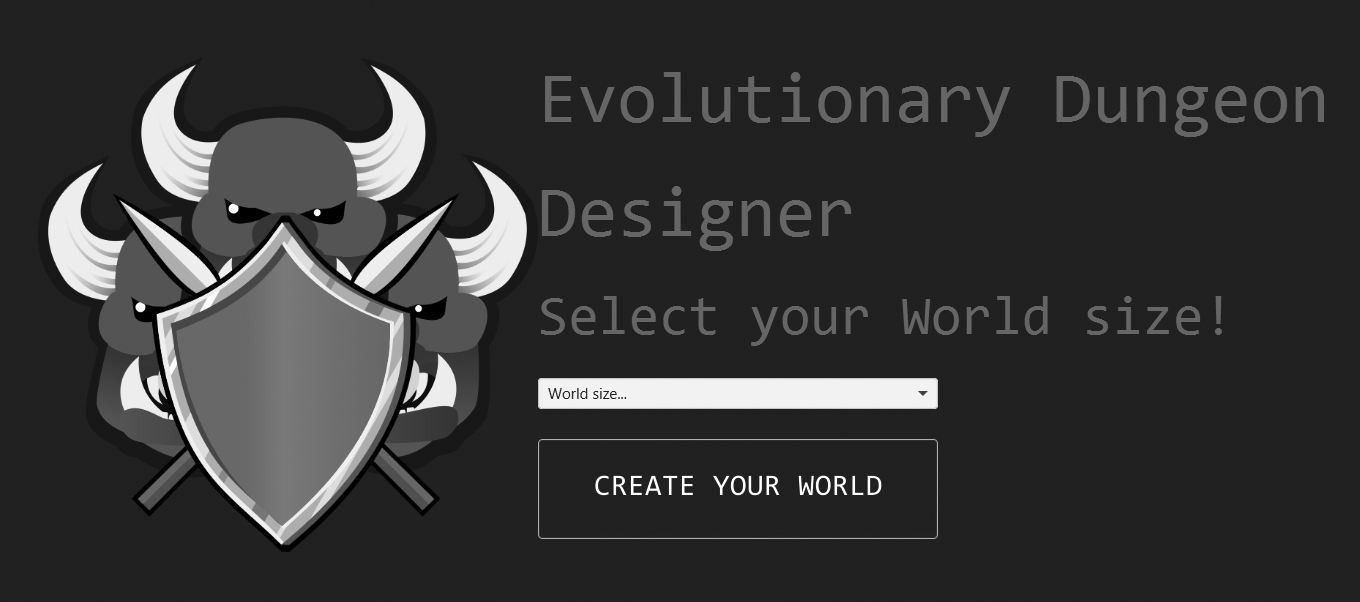
\includegraphics[width=1\columnwidth]{included-papers-tex/paper-1/figures-extra/start-edited.png}
    \caption{The start screen lets users choose the dungeon dimensions.}~\label{p1fig:launch}
\end{figure}

Previous research presented the \emph{Evolutionary Dungeon Designer} (EDD)~\citepone{p1Eddy1_5, p1Eddy2} as a mixed-initiative authoring tool for designing dungeon rooms for adventure games. EDD automatically generates and suggests rooms to the user while the user is manually designing one of them. The user either form the room from scratch or from a previously generated suggestion. This is done by means of a FI-2Pop GA~\citepone{p1kimbrough_feasibleinfeasible_2008}, where game design patterns are used both as input parameters and as objectives. These patterns involve micro-patterns (\textsc{Enemy}, \textsc{Treasure}, \textsc{Chamber}, \textsc{Corridor}, \textsc{Connector}, \textsc{Entrance}, and \textsc{Door}) as well as meso-patterns (\textsc{Ambush}, \textsc{Guard Chamber}, \textsc{Treasure Chamber}, and \textsc{Guarded Treasure}). EDD also ensures that all generated rooms are playable.

Initial experiments on EDD~\citepone{p1Eddy1_5} validated its PCG system in terms of fitness optimization, pattern detection, and solution diversity, providing a sufficient level of control to the designer. The following iteration~\citepone{p1Eddy2} explored the capabilities of EDD as a mixed-initiative level generator as a means of facilitating collaboration between human designers and PCG algorithms. Among its key features, the participants of a user study highlighted EDD as a useful framework for working with game design patterns in the context of search-based problems. The suggestions were considered a good source of inspiration as well as time saving. This user study also shaped the roadmap for future improvements on EDD. This included extending EDD from room generation to complete dungeon generation, and preserving the users' designs to a higher degree in relation to both design patterns and room aesthetics.

This version of EDD extends previous work based on the aforementioned user study by implementing the following key improvements:

\begin{itemize}
  \item The designer is now able to construct, develop, and edit a grid-based dungeon of different dimensions and inter-connected rooms, in contrast to a single room, which in turn, helps the designer on having context over their work on individual rooms and giving them more freedom on producing variations.
  \item The designer receives extended information about the consequences of their changes in individual rooms, and the differences between the current edited room and the proposed suggestions by the EA.
  \item The UI has been renovated to account for the newly added features by means of different views and options, as well as, a better structure and distribution of the different elements in the generator.
  \item Navigation tools have been added within a view and between views, which provides an overview of the dungeon, along with a better context of the edited room.
  \item The EA has been updated to assess and preserve the aesthetic criteria of the designer by means of a new capability of locking sections of an edited room for preserving custom aesthetic structures, and by extending the evaluation function through the measurement of symmetry and similarity in the provided suggestions, both which are further explained in \citepone{p1Eddy2_5}.
\end{itemize}

\subsection{Improving the Mixed-Initiative Evolutionary Dungeon Designer} \label{p1approach}

\cref{p1fig:launch} shows the start screen in EDD, which starts a new workflow by prompting users to choose the maximum number of rooms in the dungeon to be developed. The dimensions range from 2x2 rooms up to 7x7 rooms in a square dungeon grid (also referred as world grid). From this point, the workflow offers users three different views: 1) a world view for dealing with aspects regarding the dungeon as a whole; 2) a room view which places the focus in a particular room in the dungeon; and 3) the suggestions view, which produces six different suggestions with diverging room configurations (e.g. more corridors or more chambers) for the user to choose from. The user can freely alternate between views during the design process. The current dungeon layout can be saved at any moment from either of the views.

\begin{figure}[t]
    \centering
    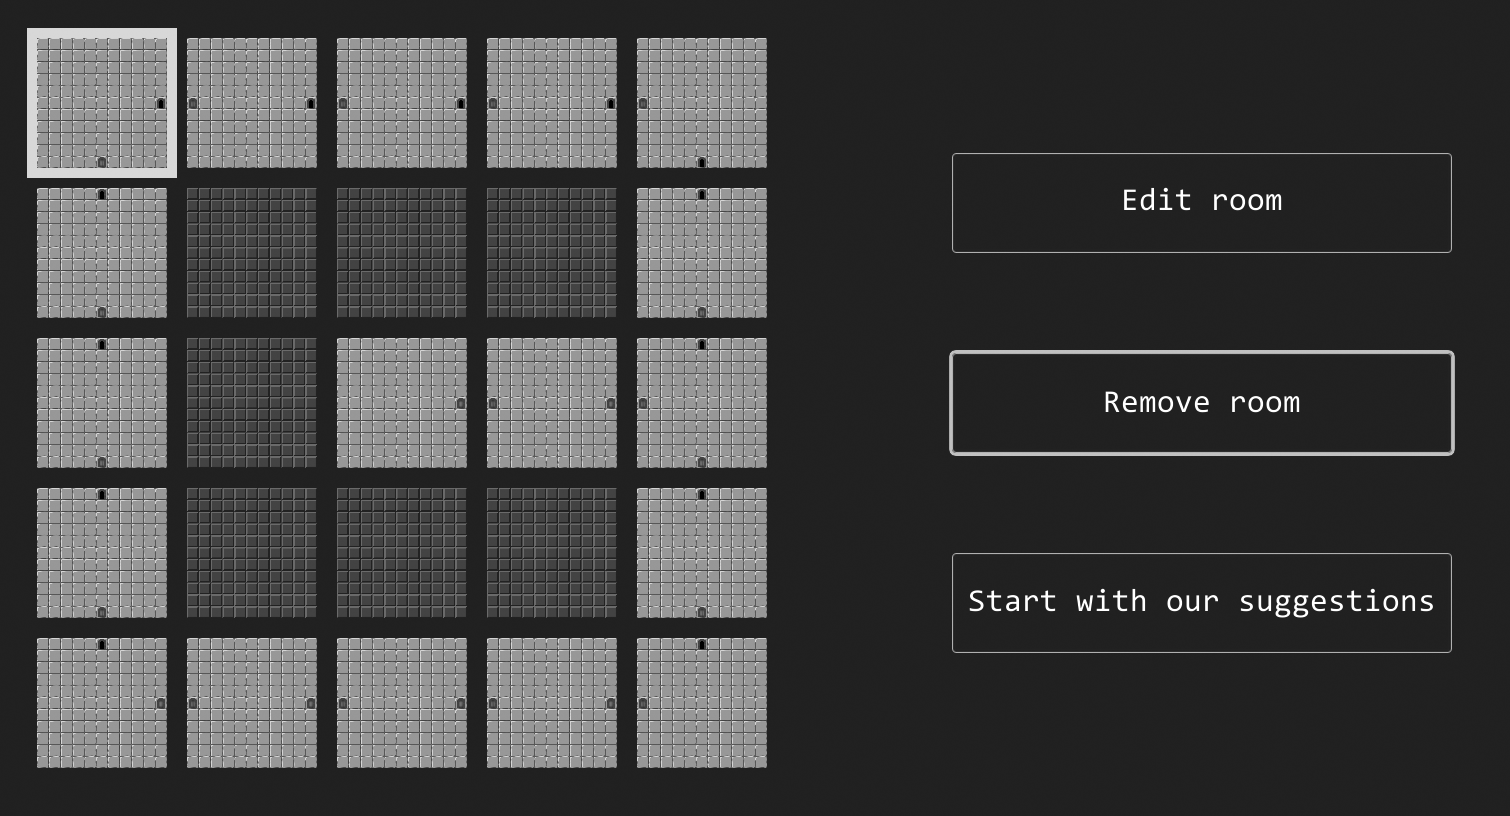
\includegraphics[width=\columnwidth]{included-papers-tex/paper-1/figures-extra/world-edited.png}
    \caption{Sample world view showing a 5x5 dungeon with 7 disabled rooms. User actions are displayed in the rightmost buttons.}~\label{p1fig:world}
\end{figure}

The world view (\cref{p1fig:world}) opens up right after the start screen, displaying a grid of the selected size composed by a fully connected set of empty rooms (all rooms are connected to their neighbors). The users can load a previously saved dungeon design, skipping the start screen and resume work from the state in which the dungeon design was saved.

From the world view users can then click and select any room to:
\begin{itemize}
\item disable or enable the room. Disabling makes the room inaccessible, removing all doors from the adjacent rooms. This can be undone by clicking \emph{enable}. Single rooms that become isolated after all their neighbors have been disabled, are automatically disabled as well. \cref{p1fig:dungeon1,p1fig:dungeon2} show two examples of dungeons with several disabled rooms,
\item get procedurally generated suggestions for that room in the suggestions view,
\item load the room in the room view for manual editing.
\end{itemize}

\begin{figure}[!ht]
    \centering
     \subfloat[\label{p1fig:dungeon1}]{%
       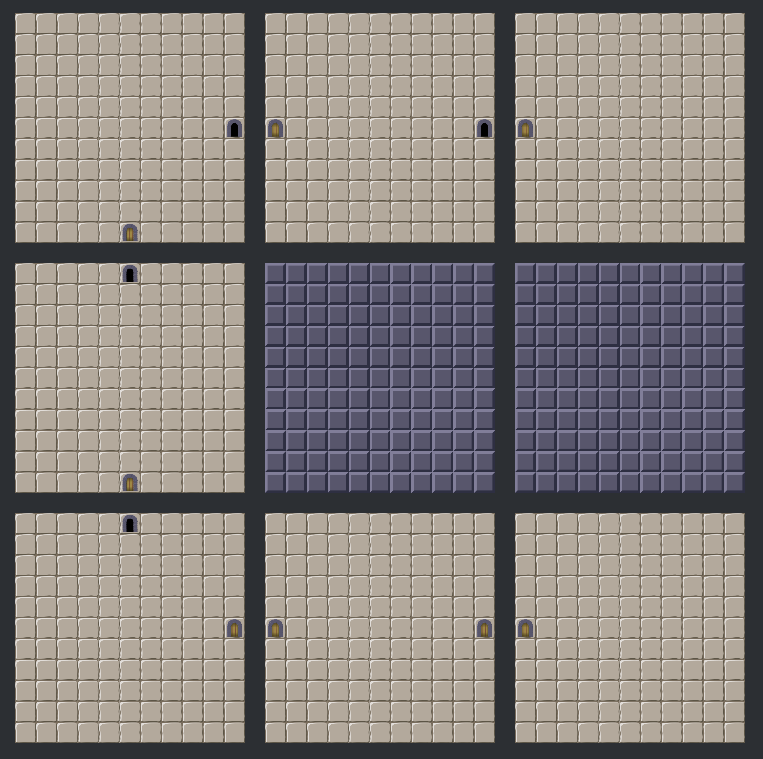
\includegraphics[width=0.49\textwidth]{included-papers-tex/paper-1/pap1-Figures/dungeon1.png}
     }
     \hfill
     \subfloat[\label{p1fig:dungeon2}]{%
       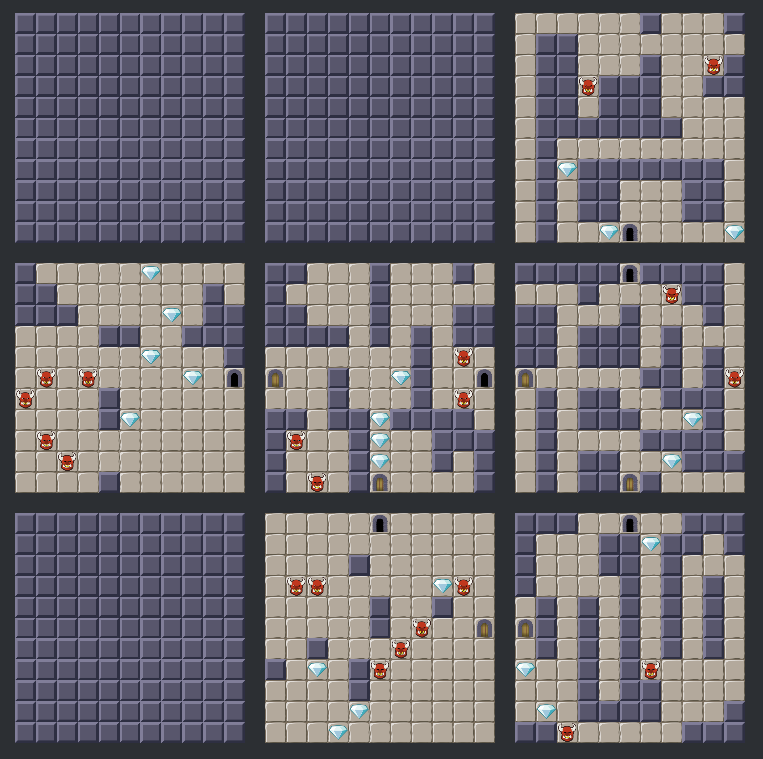
\includegraphics[width=0.49\textwidth]{included-papers-tex/paper-1/pap1-Figures/dungeon3-edited.png}
     }
    
    \caption{(a) 3x3 dungeon with 2 disabled rooms and 7 empty rooms, and (b) 3x3 dungeon completed dungeon with 3 disabled rooms.}
    \label{p1fig:dungeonsp1}
\end{figure}

\subsubsection{The Suggestions View}

By selecting ``Start with our suggestions'' in the world view (\cref{p1fig:world}) six uniquely generated rooms are presented to the user in a separate window: the suggestions view (\cref{p1fig:suggestionsview}). When clicking any of the suggestions, it will replace the previously selected room in the dungeon.

\begin{figure}[!ht]
    \centering
    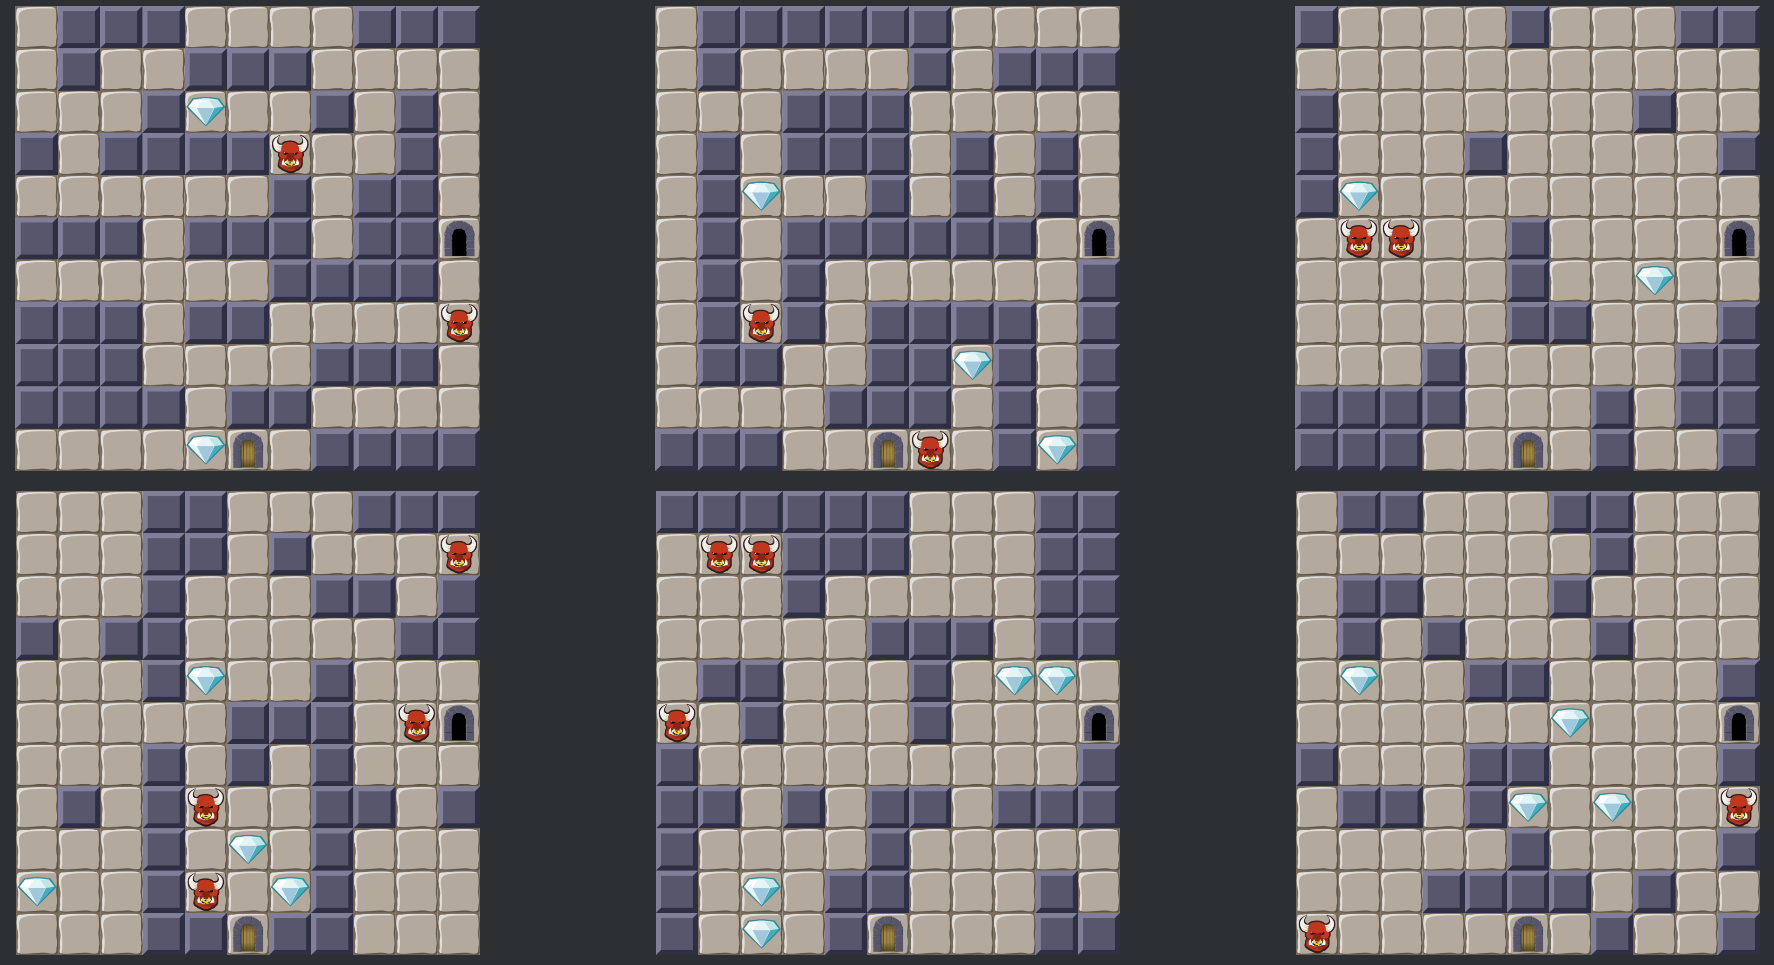
\includegraphics[width=\columnwidth]{included-papers-tex/paper-1/pap1-Figures/suggestionsview.png}
    \caption{Six procedurally generated rooms presented to the user in the suggestions view.}~\label{p1fig:suggestionsview}
\end{figure}

A similar functionality was present in the former version of the tool, presented only once as the start screen. Now users can freely alternate between the world and the suggestions views, getting as many suggestions as they need, deciding whether to start creating every room from a clean state or to get inspiration from one of the generated rooms.

\begin{figure*}[t]
    \centering
    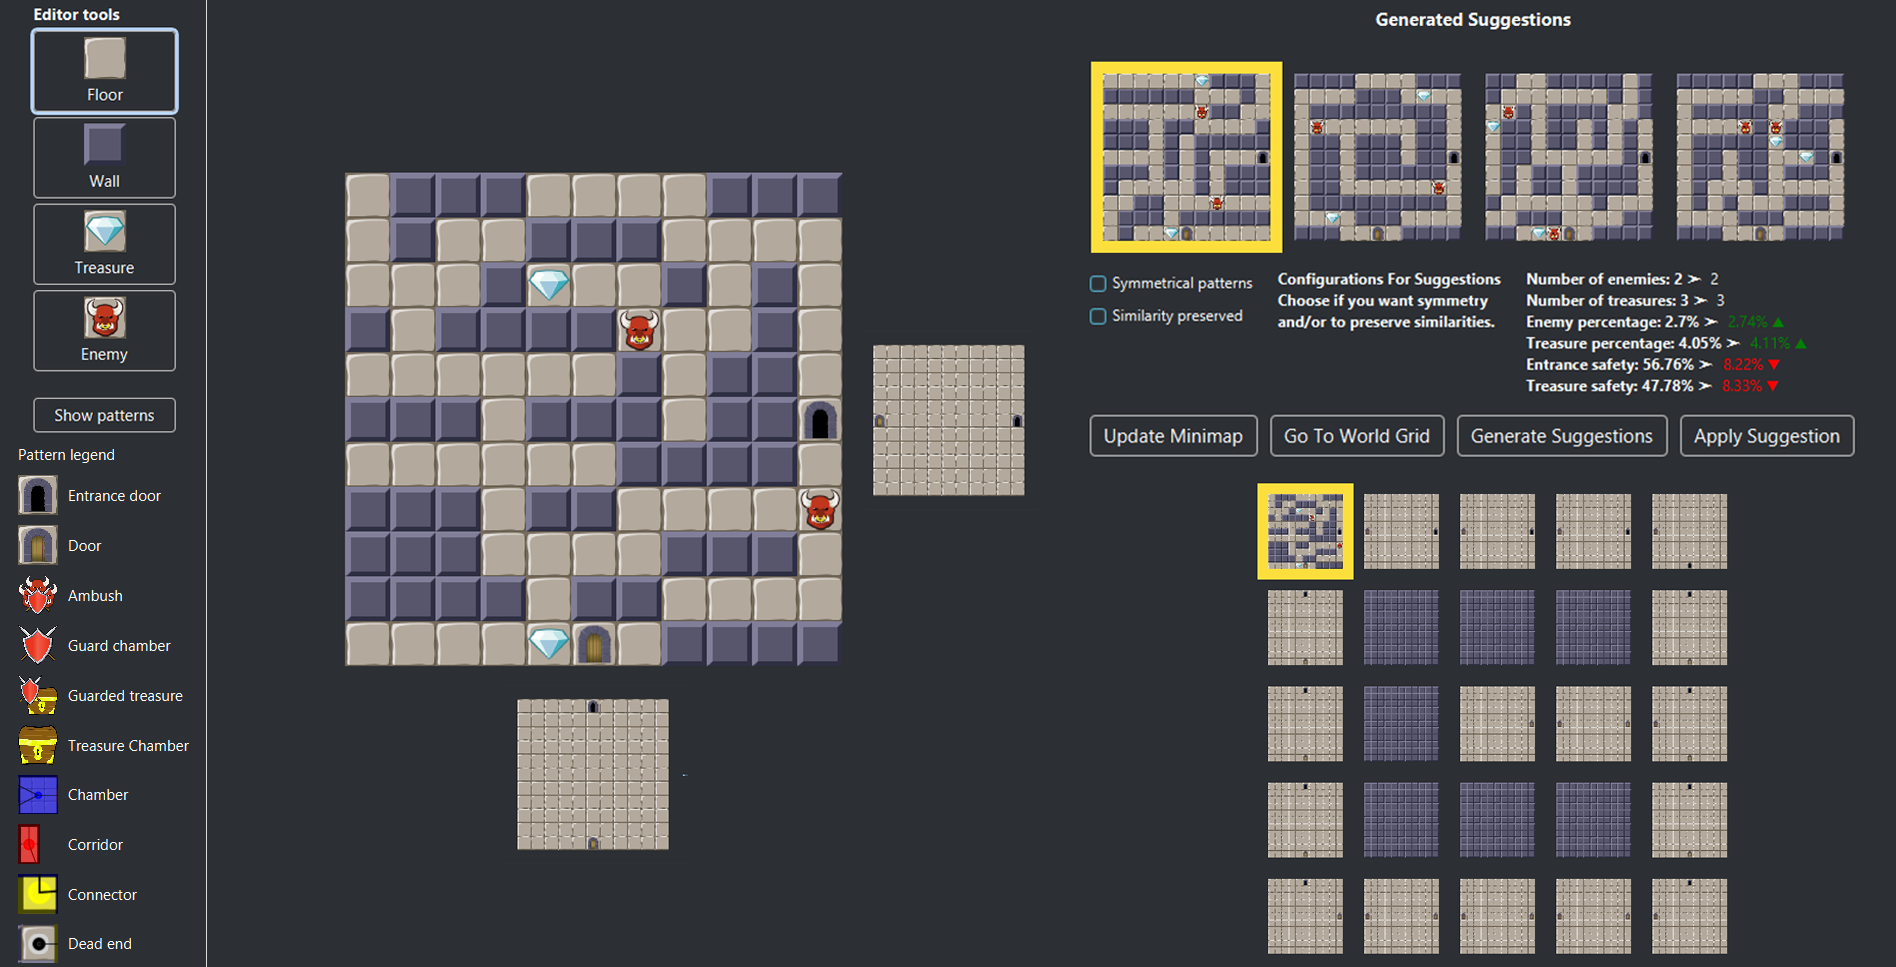
\includegraphics[width=\textwidth]{included-papers-tex/paper-1/pap1-Figures/roomview.png}
    \caption{The room view while editing the top-left corner in a 5x5 dungeon with seven disabled rooms.}~\label{p1fig:roomview}
\end{figure*}

Suggestions preserve the door layout from the room that was selected in the world view. The suggestions shown in \cref{p1fig:suggestionsview} have been created for the room selected in \cref{p1fig:world}, placed in the top-left corner, and containing only two doors connecting them to their east and south neighbor.

\subsubsection{The Room View}

\begin{table*}[ht]
% \centering
\caption{General consensus on EDD's features} \label{p1tab:consensus}
\resizebox{0.8\textwidth}{!}{
\begin{tabularx}{\textwidth}{|p{0.2\textwidth}|p{0.99\textwidth}|}
\cline{1-2}

Description & Participants’ Consensus \\\cline{1-2}
World Grid  of the dungeon                   & Its purpose of establishing an illusion of a fully realized dungeon is somewhat achieved. However, limitations exist with how it defines feasibility, a dungeon’s starting point, and the entrances, which disrupts the designers’ decisions.                                                                                                                                                                                   \\\cline{1-2}
World View                                  & The world view’s usefulness for the most part could not be established, other than for the purpose of going to the suggestions view (which was already seldom during the user study) and having a closer look at the entire dungeon without any distractions. Some participants preferred features to be already in the room view’s minimap, and some wanted to see more specific functionalities within the world view itself. \\\cline{1-2}

Enabling and  \newline disabling rooms                & As the user study restricted participants to create 3x3 dungeons, this feature for the most part has been neglected. This is also in part because of its accessibility only being in the world view, which proved to be an inefficient view in general. However, its use for bigger dungeon sizes later on was appreciated, especially for more intricate design purposes.                                                      \\\cline{1-2}
Suggestions View                            & Similarly to enabling and disabling rooms, it was quite difficult to encourage the use of this functionality due to the world view’s inefficient usability. However, this could also be due to the dungeon’s small size, as some participants expressed high interest in using more suggestions with larger dungeon sizes.                                                                                                      \\\cline{1-2}
Minimap  \newline  navigation                      & The minimap proved to be a strong tool not only for navigation purposes, but also for supporting design decisions and choices. The directional buttons were rarely used, but their room previews were helpful in emphasizing the current room’s connection to adjacent rooms without looking at the minimap. On the other hand, this lowered the usability of the world view.                                                   \\\cline{1-2}
Parameters                                       & The parameters were, in general, lacking. They served to be important in decision-making when choosing a suggested map in room view, but there were still doubts on their accuracy and sufficiency when providing information about the generated suggestions.                                                                                                                                                                       \\\cline{1-2}
Generated maps for  \newline  suggestions in room view & Suggestions in the room view proved to be very helpful in supporting the whole design process as they primarily acted as inspirations for the users. The most prominent comment among the users is the preference of having more control on how suggestions should be generated depending on different types of parameters.                                                                                                     \\\cline{1-2}
Design \newline  patterns& The patterns’ visualization was, in general, lacking and not self-explanatory. Some participants have expressed interest in using patterns as a parameter in the generation of suggestions.                                                                                                                                                                                                                                     \\\cline{1-2}
Dark theme                                  & EDD’s dark theme for the user interface received a positive response as it makes working with the program easier.
	\\ \cline{1-2}
\end{tabularx}
}
\end{table*}

% \begin{table}
% \begin{center}
% {\caption{Best performing setups based on their internal validation and visualization of clustered data points.}\label{table:setups}}
% \resizebox{\textwidth}{!}{
% \begin{tabular}{ccccccc}
% \hline
% \rule{0pt}{12pt}
% Algorithm&Data&K&$\Diamond$&$\Box$&$\bigtriangleup$ 
% \\ 
% \hline
% \\[-6pt]
% K-Means & Tiles-PCA & 9 & 0.43 & 0.73 & 9438.233 \\ 
% K-Means & Tiles-PCA & 12 & 0.41 & 0.77 & 9436.928 \\
% K-Means & Dimensions-PCA & 12 & 0.43 & 0.73 & 7738.343 \\
% Agglomerative single & Combined-PCA & 6 & 0.51 & 0.43  & 38.833 \\ 
% Agglomerative avg. & Dimensions-PCA & 6 & 0.44 & 0.67 & 3463.567 \\ 
% \hline
% \\[-6pt]
% \multicolumn{6}{l}{$\Diamond$ Silhouette Score\ \
% $\Box$ Davies Bouldin Index\ \
% $\bigtriangleup$ Calinski-Harabasz Index}
% \end{tabular}
% }\end{center}
% \end{table}

Users edit single rooms in the room view (\cref{p1fig:roomview}), regardless of whether these are new empty rooms, procedurally generated suggestions, or previously edited rooms. The room view is an improved and extended version of the main screen in the last version of EDD~\citepone{p1Eddy2}. All functionalities from that version are still present: manually editing the room by changing tiles (floor, wall, enemy, and treasure), displaying an overlay view of the existing design patterns, and procedurally generating suggestions based on the current edited room's configuration.

Navigation is one of the crucial added features, allowing users to move around the dungeon without going back to the world view. Two other options offer navigation through the dungeon: the navigational buttons and the minimap. The navigational buttons are displayed next to each of the edited rooms' borders that contain a door. Provided that the room being edited in \cref{p1fig:roomview} is located in the top-left corner, two navigational buttons are displayed right and below the room, respectively. Clicking a navigational button transports the user to that room, replacing the currently edited room with the targeted neighbor. Instead of using arrows or any other fixed picture, these buttons preview the neighboring rooms as a hint for users to help them design the room currently being edited. The navigational buttons are automatically refreshed to reflect up-to-date changes performed to the neighboring rooms.  

The minimap displays a scaled-down overall picture of the whole dungeon, highlighting the currently edited room with a yellow border. Users can navigate to any room, which is not disabled and is displayed on the minimap by clicking on it, replacing the current room. The buttons above the minimap allow users to go \textit{Back To World Grid}, to \textit{Update Minimap}, as well as request and select procedurally generated suggestions. The whole minimap is updated whenever the user navigates to a different room, but if the user wants to see the last changes applied to currently edited room reflected on the minimap, a manual refresh has to be done. This is done to reduce the workload derived from re-rendering the minimap automatically after every manual edition.

The generated suggestions work similarly to the previous version of EDD: four unique maps are generated by the underlying evolutionary algorithm in four subsequent evolutions, seeding the four initial populations with different sets of features extracted from the edited room. Each suggestion is evolved by means of a different fitness function, therefore addressing different goals to maximize diversity in the provided suggestions. Clicking on a suggestion highlights it, and clicking \textit{Apply Suggestion} replaces the current room with the highlighted map. This differs from the previous version, in which maps were applied at the moment they were clicked on, occasionally causing work loss due to accidental replacements. 

Additionally, highlighted suggestions display informative parameters below them. These describe meaningful features of the highlighted room that are relevant to both the human designer and the evolutionary algorithm's fitness calculation: number of enemies and treasures, enemy and treasure rate (in relation to floor tiles), and entrance and treasure safety (see \citepone{p1Eddy1_5} for a detailed description). These parameters are displayed as a comparison between their values in the edited room and in the highlighted suggestion, showing how they would change if the suggestion is applied. 

Two checkboxes below the suggestions now offer users the possibility to ask specifically for the provided suggestions to address symmetry and similarity aesthetic features, respectively. By ticking the symmetry checkbox, two of the suggestions will be generated by the evolutionary algorithm using a symmetry fitness function, which enable the generation of symmetric rooms, (either vertically, horizontally, or diagonally). Analogously, ticking the similarity checkbox, the other two suggestions are generated with a similarity fitness function, which promotes the generation of room aesthetically similar (but never equal) to the currently edited map. These fitness functions are presented in~\citepone{p1Eddy2_5}. When both checkboxes are unchecked, the fitness functions described in~\citepone{p1Eddy2} are used.

\subsection{User Study} \label{p1userstudy} 

\begin{table}[ht]
% \centering
\caption{Participants’ most requested features} \label{p1tab:demands}
% \resizebox{\paperwidth}{!}{\begin{minipage}{\paperwidth}
\resizebox{0.8\textwidth}{!}{
% \begin{tabularx}{\textwidth}{|p{0.2\textwidth}|p{0.99\textwidth}|}
\begin{tabularx}{\textwidth}{|p{0.2\textwidth}|p{0.99\textwidth}|}
\cline{1-2}
Feature                                 & Description                                                                                                                                                                                                                                                                                                                                                                                                         \\\cline{1-2}
Design patterns                   & Their visualization and accuracy should be improved. Other than acting as visual guide for map information, they should be used to help generate rooms as well. They should also be available for the entire dungeon.                                                                                                                                                                                 \\\cline{1-2}
Parameters                                  & They need to have more information about the specific room, and have better visualization in order to make the designer trust their accuracy more. The parameters should also consider the entire dungeon as a whole in different terms such as difficulty and balance.
\\\cline{1-2}
Generated suggestions               & In general, the participants want more variety and control in the generation of suggestions using different types of parameters e.g. their degree of similarity and fitness functions.                                                       \\\cline{1-2}
Redefined feasibility                           & Eddy 3.0’s definition of feasibility should be revised which considers the whole dungeon and its connected rooms.                                                                                                      \\\cline{1-2}
World View                      & The World View should be revised and enhanced with more special features which would encourage users to visit it more.                                                    \\\cline{1-2}
World grid                                       & The computation of the whole dungeon should be improved. It should have an option to define a starting point. Its definition of entrance doors should be improved, as well as the calculation of distances of tile types.                                                                                                                                                                       \\\cline{1-2}
Version control & Some participants want to preview suggestions within the Room View to help their judgment and the ability to save suggestions for later use. They also want to revert to old designs in case they have second thoughts.                                                                                                     \\\cline{1-2}
Templates                             & Some participants want the ability to save their own manual designs to be carried over to other grids.                                                                                                                                                                                                                                     \\\cline{1-2}
Automated assistance                                  & The participants in general welcome a bit more automated assistance when doing manual designs, which can reduce clicking around the program. It should also not be too invasive for the designer. 
	\\ \cline{1-2}
\end{tabularx}
}
% \end{minipage}}
\end{table}

% \begin{table}[h]
% \centering
% \caption{Developed game based features used as dimensions in the~\acrlong{icmape}}\label{table:mape-dimensions}
% % \resizebox{\textwidth}
% % \resizebox{\textwidth}
% \begin{tabularx}{\textwidth}{|c|X|}
% \cline{1-2}
% \rule{0pt}{12pt}
% Feature&Definition\\ \cline{1-2}
% % \\[-6pt]
% Similarity & Refers to the aesthetic (tile-by-tile) similarity between a room and the current designer's design.\\ \cline{1-2}
% Inner Similarity & Refers to the similarity of the sparsity and density of the different tile types of a room designer's current design.\\ \cline{1-2}
% Symmetry & Refers to the aesthetic symmetry of a room.\\ \cline{1-2}
% Leniency & Refers to how challenging rooms are; calculated based on the position of enemies and balance between enemies and treasures.\\ \cline{1-2}
% Linearity & Refers to the amount of paths connecting doors within a room; calculated based on how many spatial patterns are traversed.\\ \cline{1-2}
% \#Meso-Patterns & Refers to the number of meso-patterns that exist within a room, normalized by an estimated maximum number based on the room's size and the minimum chamber size.\\ \cline{1-2}
% \#Spatial-Patterns & Refers to the number of spatial-patterns that exist within a room, which can be chambers, corridor, turns, junctions, and intersections.\\ \cline{1-2}
% \end{tabularx}
% \end{table}

A user study was conducted in order to assess the impact on the design process caused by the improvements made to EDD. Five game developers participated in the study, which had the following structure:
\begin{itemize}
\item \textit{Introduction to the purpose of the study}. Participants were asked whether they were familiar with the previous version of EDD.
\item \textit{Demonstration of the tool}, showcasing its workflow and features with a short example performed over a 3x3 dungeon. 
\item \textit{Designing a dungeon}. After the demonstration the users were tasked to design a 3x3 dungeon within approximately 10 minutes, saving the work after that for a later analysis and discussion conducted in a structured interview with the participant after this phase. Two observers took notes of what the participant was doing, providing additional data for the later analysis.
\item \textit{Questionnaire}. The users were asked a few questions regarding their background in game design as well as dungeon-based games. They were also asked whether they had any previous experience with mixed-initiative tools.
\item \textit{Interview}. A semi-structured interview was conducted to provide data for an analysis and discussion about the tool, and its improvements. Audio was recorded for a later analysis.
\end{itemize}

As as result of the questionnaire, the following information was gathered from the participants:
\begin{itemize}
\item User 1 has been working for more than ten years in the game industry as a data scientist and user experience researcher. The user holds prior experience with RPGs and dungeon crawlers, and is familiar with the terms of mixed-initiative tools and has used The Sentient Sketchbook in the past. This user is the only one who participated in the former user study of EDD.
\item User 2 has been working for six months as a project coordinator of eSports events and has long experience of playing dungeon crawlers and RPGs. This user is not familiar with mixed-initiative concepts and has never used a mixed-initiative authoring tool before.
\item User 3 has been working for six years in the game industry as a user experience researcher and a biometrics expert. The user has prior experience with dungeon style games, but has limited knowledge about mixed-initiative tools.
\item User 4 has been working for nine years as a senior user experience researcher and has long experience of playing dungeon crawlers and RPGs. This user is not familiar with mixed-initiative concepts and has never used a mixed-initiative authoring tool before. 
\item User 5 has been working for three weeks as a game user researcher. This user has no experience with dungeon crawlers and dungeon-based RPGs, and is not familiar with mixed-initiative tools. 
\end{itemize}

\subsection{Results and Discussion} \label{p1conclusion} 

As with any raw qualitative data, the data collected from the user study has to go through a condensation process in order to isolate the most relevant information that will answer the research questions. In a blueprint provided by~\citepone{p1srnka2007words}, the qualitative data obtained has undergone four out of five stages: 
\begin{itemize}
\item \textit{Material sourcing}: an audio recording the user study, interview materials, and the authors’ own observations.
\item \textit{Transcription}: combining and writing down the observations and questionnaire answers for each participant in the user study.
\item \textit{Unitization}: dividing the data according to the mixed-initiative features of EDD.
\item \textit{Categorization}: dividing the data according to categories relevant to the research questions while taking into consideration the principles of mixed-initiative.
\end{itemize}

All participants in the user study perceived EDD as overall good and intuitive. \cref{p1tab:consensus} shows their general consensus of EDD's usability and capability to foster creativity in dungeon design. \cref{p1tab:demands} lists the participants' most requested missing features.

The main goal of mixed-initiative interaction pertains to the flexibility of roles between the human and computer as a team and simplifying the general experience~\citepone{p1allen1999mixed}, and this was somewhat achieved by EDD. This could be proven by how features such as suggestions and the implementation of a whole dungeon with navigation have definitely supported the users when making decisions throughout the design process. As a result the experience was overall simple and intuitive. It could not be said, however, that the set goal has been fully achieved; a fully successful mixed-initiative system emphasizes interchangeable roles of the human and computer while maintaining the balance between them. The participants in the user study did not feel restricted, but they still desired more control in EDD’s assistance in the design process, as well as different suggestions that the designer cannot come up with themselves.

\citepone{p1horvitz1999principles} provides a list of principles for mixed-initiative user interfaces which would enhance human-computer interaction. EDD has achieved four out of twelve in Horvitz’s list of critical factors that would make up a fully successful mixed-initiative system:

\begin{itemize}
\item \textit{Developing significant value-added automation}: providing an automated solution that cannot be achieved with direct manipulation. EDD provides a framework for the generation of complex dungeons of different sizes, together with suggestions of similar dungeon rooms and information parameters for these suggestions. 
\item \textit{Considering uncertainty about a user’s goals}: taking advantage of a user’s uncertainty in their intentions. EDD provides the choice to initialize rooms in a dungeon with either an empty slate or from any of the generated suggestions.
\item \textit{Inferring ideal action in light of costs, benefits, and uncertainties}: considering the value of an automated service in regards to the usually expected value of taking actions. EDD’s main motivation is to significantly reduce the cost of game design while maintaining and improving creativity, which has at least partially been fulfilled.
\item \textit{Employing dialogue to resolve key uncertainties}: establishing an efficient dialog between the human and computer when uncertainty arises while considering the costs of potentially disrupting the user. EDD extracts and displays relevant features in the edited and suggested rooms for the users to guide their decisions. The minimap also fulfill parts of this role.
\end{itemize}

There are other principles which are relevant to EDD which fall in line with the participants’ feedback. For example, some principles such as the ability to continuously learn from the user’s input and to preserve memory of their decisions and actions may pertain to the desired features of having more control in the generation maps and receiving more assistance in preserving their own manual designs for different purposes.

\subsection{Conclusions and Future Work}

The contributions presented in this work explore how the user interface and the mixed-initiative aspects in the Evolutionary Dungeon Designer have been improved, as well as how they should be improved on further in order to increase creativity during the dungeon design process.

The addition of the world grid provides the adoption of a new workflow, which offers users the possibility to start designing either from empty rooms or PCG suggestions. Various changes in the user interface were made to accommodate the increased dungeon size. With a larger dungeon, navigation has proved to be a key functionality, as well as giving an overview of the adjacent rooms. Now users can get a better understanding of the context of the room currently being edited. In conjunction with the navigation and larger dungeons, a minimap was also added to further enhance the experience when designing a larger dungeon. Alongside these changes, aesthetic goals have been included in the generative process. Visual cues for room descriptors were added, so that the user can make a more informed decision when selecting suggested maps.

Compared to its previous version, EDD further empowers the mixed-initiative design process by providing more context, feedback, flexibility, and to some extent, the ability to address aesthetic features in the procedural suggestions. Creativity can directly adhere to the amount of interesting possibilities a designer can employ, which is relevant to providing rich contexts to dungeon designs. EDD offers a mixed-initiative experience that provides adequate flexibility for the designer’s intentions as the results from the user study have shown.

Overall, our user study successfully shows the strengths of mixed-initiative tools for designers but it also reveals various limitations, which should be considered by the community when creating a mixed-initiative tool.

To a certain extent, controllability is preferred than expressivity, as the users continuously try to impose their vision, which is a non-trivial task for automated systems to capture, thus, the users are more likely to sacrifice to a certain degree expressivity and exploration of the tool by gaining control over the generated content. 

The capability of proposing useful and novel suggestions is fundamental to fostering creativity and impulses the generation of more interesting content. Moreover, explicit information about the designers’ changes and choices is important as it helps them understand the effect of their decisions. 

Finally, this work has identified features that should still be taken into consideration for future versions of the tool, which are shown in \cref{p1tab:demands}.

\subsection*{ACKNOWLEDGMENTS}
The Evolutionary Dungeon Designer is part of the project \textit{The Evolutionary World Designer} which is supported by The Crafoord Foundation.

% \let\oldthebibliography=\thebibliography
% \renewenvironment{thebibliography}[1]{%
%   \oldthebibliography{#1}%
%   \setcounter{enumiv}{0}%
% }

% \bibliographystyle{ieeetr}
\bibliographystylepone{ieeetr}
% \phantomsection
% \addcontentsline{toc}{section}{REFERENCES}
\bibliographypone{included-papers-tex/paper-1/references}

\setcounter{figure}{0}    
\setcounter{table}{0}    
\setcounter{footnote}{0}      

% \clearpage
%\includedPaper{\textsc{paper ii - assessing aesthetic criteria in the evolutionary dungeon designer}}{\textsc{paper ii - assessing aesthetic criteria in the evolutionary dungeon designer}}{Alberto Alvarez, Steve Dahlskog, Jose Font, Johan Holmberg, and Simon Johansson}

\includedPaper{\textsc{paper ii - assessing aesthetic \\ criteria in the evolutionary \\ dungeon designer}}{\textsc{paper ii - assessing aesthetic criteria in the evolutionary dungeon designer}}{Alberto Alvarez, Steve Dahlskog, Jose Font, Johan Holmberg, \\ and Simon Johansson}

% \section{\textsc{paper i - fostering creativity in the mixed-initiative evolutionary dungeon designer}}

% \vspace{-10pt}
% \textit{Alberto Alvarez, Steve Dahlskog, Jose Font, Johan Holmberg, Chelsi Nolasco, and Axel Österman}

\normalfont
\textbf{\textsc{ABSTRACT}}

The Evolutionary Dungeon Designer (EDD) is as a mixed-initiative tool for creating dungeons for adventure games. Results from a user study with game developers positively evaluated EDD as a suitable framework for collaboration between human designers and PCG suggestions, highlighting these as time-saving and inspiring for creating dungeons.

Previous work on EDD identified the need of assessing aesthetic criteria as a key area for improvement in its PCG Engine. By upgrading the individual encoding system and the fitness evaluation in EDD's evolutionary algorithm, we present three techniques to preserve and account the designer's aesthetic criteria during the dungeon generation process: the capability of locking sections for preserving custom aesthetic structures, as well as the measurement of symmetry and similarity in the provided suggestions.

\textbf{\textsc{PUBLISHED IN}}

Proceedings of the 13th International Conference on the Foundations of Digital Games, ACM, 2018

\section*{ASSESSING AESTHETIC CRITERIA IN THE EVOLUTIONARY DUNGEON DESIGNER}

\subsection{Introduction} \label{p2introduction}

%\begin{itemize}
%  \item Evolutionary approaches to design of dungeons
%  \item Different criteria evaluated in dungeons
%  \begin{itemize}
%  	\item Criteria evaluated for evolutionary approaches
%  \end{itemize}
%  \item What we present in the paper  Techniques and changes. How is the paper divided
%\end{itemize}

%Procedural content generation (PCG) has been widely used to generate content in games for different reasons, due to constraints in memory~\citepsecond{p2Braben1984Elite}, create new experiences for the user~\citepsecond{p2Toy1980Rogue}, animations~\citepsecond{p2Maxis2008Spore} or more recently, to create most of the assets~\citepsecond{p2HelloGames2016NoSky}. Moreover, the interest on PCG has increased since researchers explore ways to automatize, reduce cost and, produce novel and interesting content, for instance, weapons~\citepsecond{p2Hastings2009GalacticGame}, levels~\citepsecond{p2Shaker2012EvolvingEvolution}, music and sound~\citepsecond{p2Hoover2011InteractivelyScaffolding,Scirea2017PImprovisation}, generators \citepsecond{p2Liapis2013SentientAuthoring} and even complete commercial games with their own rules \citepsecond{p2Browne2007Yavalath}.
Procedural content generation (PCG) has been widely used to generate content in games for different reasons, due to constraints in memory~\citepsecond{p2Braben1984Elite}, create new experiences for the user~\citepsecond{p2Toy1980Rogue}, animations~\citepsecond{p2Maxis2008Spore} or more recently, to create most of the assets~\citepsecond{p2HelloGames2016NoSky}. Moreover, interest in PCG has increased as researchers have explored ways to automate, reduce cost and, produce novel and interesting content, for instance, weapons~\citepsecond{p2Hastings2009GalacticGame}, levels~\citepsecond{p2Shaker2012EvolvingEvolution}, music and sound~\citepsecond{p2Hoover2011InteractivelyScaffolding,p2Scirea2017PImprovisation}, and even complete commercial games~\citepsecond{p2Browne2007Yavalath}.

Search-based procedural content generation (SBPCG) is a popular PCG approach that uses evolutionary algorithms (EA) for guiding the content generation process by means of evaluation functions~\citepsecond{p2Shaker2016TheApproach}. Mixed-initiative SBPCG involves human users in the evolutionary process so that promotes the co-creation of human and machine-made designs \citepsecond{p2Liapis2013SentientAuthoring}.

% \begin{figure}[H]
% 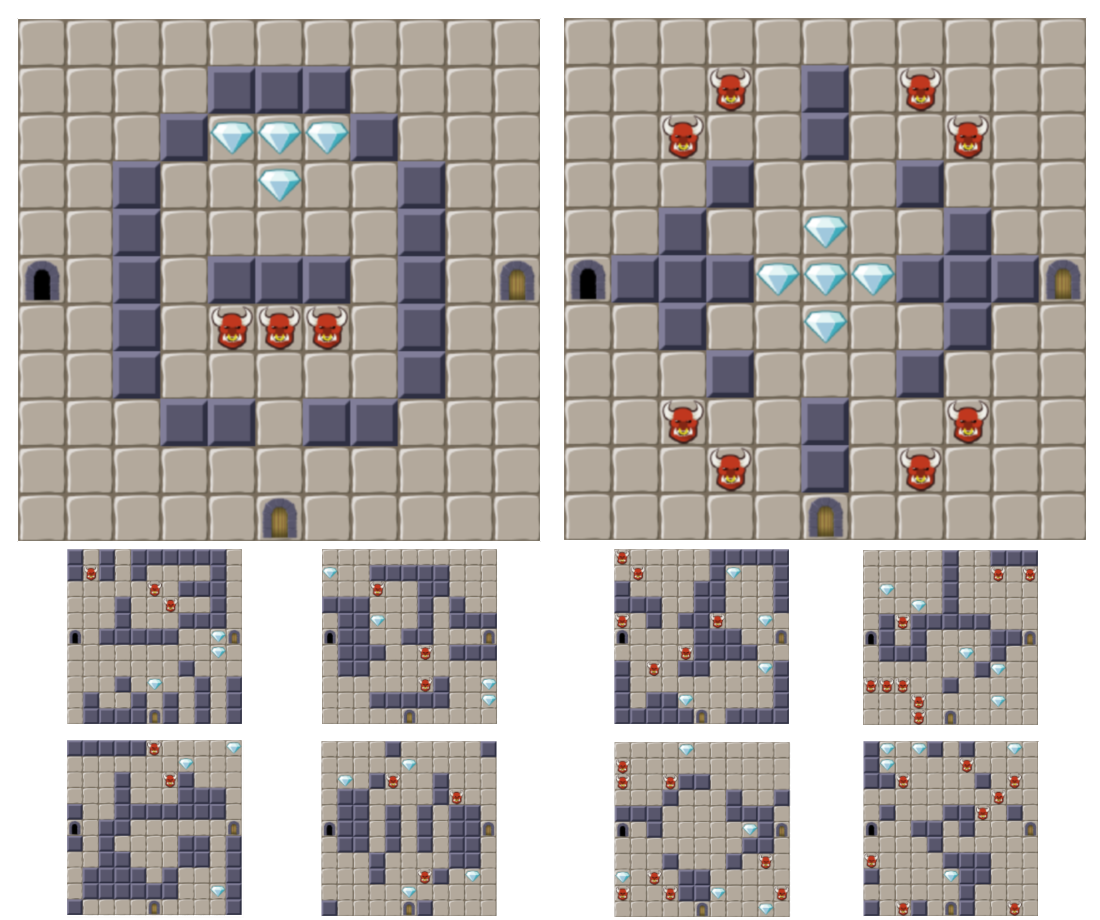
\includegraphics[scale=0.39]{Figures/figure-not-preserving}
% \caption{Sample maps from the previous version of EDD, not preserving the aesthetic changes in suggestions}
% \label{p2fig:no-aesthetic}
% \end{figure}

%The criteria can vary depending on the technique used, the goal to be reached and the evaluation to be performed. In offline generation, the algorithm tries to satisfy functional criteria (e.g. the level can be finished or all the passable tiles are accessible) \citepsecond{p2Shaker2016TheApproach,Togelius2007TowardsGames}. 
\begin{figure} [!h]
\centering
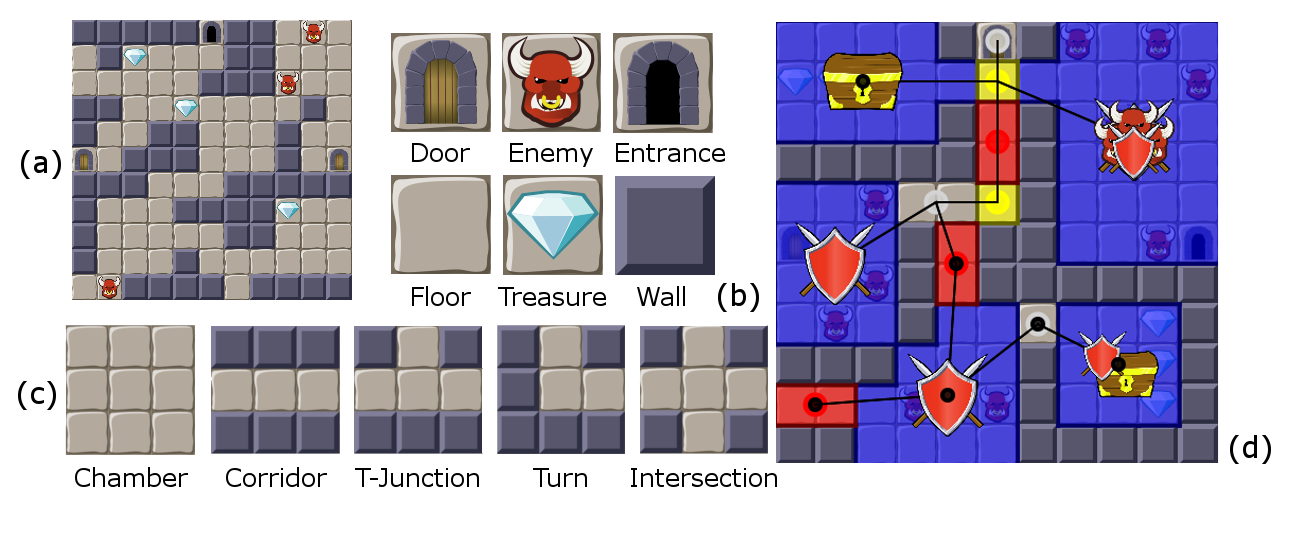
\includegraphics[width=\textwidth]{included-papers-tex/paper-2/pap2-figures/map-figure.png}
\caption{Current version of EDD and its different components. (a) Basic room, (b) different placeable tiles, (c) micro-patterns and (d) meso-patterns.}
\label{p2fig:eddy-map}
\end{figure}

As discussed by~\citepsecond{p2Baldwin2017TowardsGeneration}, it is important for a mixed-initiative SBPCG approach to evaluate the degree to which generated designs are aesthetically pleasing and interesting to the human designer. This is stressed by the designer's will to imprint and preserve their custom designs on the generated content offered by the PCG system. It is a non-trivial task to know which parts the designer wants to preserve, as well as correctly balancing human and procedurally designed content in the generated solutions. This motivates the work presented here, in which we address the need for assessing aesthetic criteria by improving both: the solution encoding mechanism and the fitness evaluation function in EDD's evolutionary algorithm.

%The overall goal of the research is to assess one of the problems that arose from the previous research's case study \citepsecond{p2Baldwin2017TowardsGeneration}, where the generator did not capture and preserve the manually edited changes done by the designers nor their aesthetic criteria in the generated suggestions. as shown in figure \ref{p2fig:no-aesthetic}. 

This paper is organized as follows: Section \ref{p2background} presents previous and related works in mixed-initiative design. Section \ref{p2approach} describes in detail the contributions of this paper and presents the results from the laboratory experiments used for validating them. Finally, Section \ref{p2conclusion} summarizes and discusses these results, as well as sets future questions to be addressed by further research in the area of aesthetic criteria and EDD.

\subsection{Related Work} \label{p2background}

\begin{figure}
\centering
\includegraphics[width=0.7\textwidth]{included-papers-tex/paper-2/pap2-figures/figure-possible-zones.png}
\caption{Different uses and possibilities that the designers can have for locking the tiles in the Room, in order to, preserve their manual changes and diverse objectives}
\label{p2fig:possible-zones}
\end{figure}


Aesthetic criteria was specified by previous research as a key feature while evaluating content, as it leads to the generation of more customized content in the eyes of the human designer, whose aesthetic vision on the content is preserved~\citepsecond{p2Liapis2012AdaptingCreation,p2Hastings2009GalacticGame,p2Machwe2006IntegratingInvestigation}.

%\emph{Tanagra}~\citepsecond{p2Tanagra2011} is used to develop 2D platform levels. The user can place different tiles, and is able to select content, which they want to keep, while Tanagra generates content around them. 

%Aesthetic criteria has been appointed by previous research as a key feature while evaluating content, as it leads to the generation of more customized content to the eyes of the human designer, whose aesthetic vision on the content is preserved \citepsecond{p2Liapis2012AdaptingCreation,Hastings2009GalacticGame,Machwe2006IntegratingInvestigation}.

Interactive evolutionary approaches incorporate human evaluation by allowing the user to select, either implicitly or explicitly, the parents of the next generation of procedurally generated individuals. In~\citepsecond{p2Zhang2015DrawCompileEvolve:Creations} system allows users to draw simple primitive shapes to seed an evolutionary algorithm and train a neural network with their aesthetic vision. In Galactic Arms Race~\citepsecond{p2Hastings2009GalacticGame} players preferences on the evolved weapons is implicitly deducted from the amount time they actively select those weapons during the gameplay.

\citepsecond{p2Liapis2012AdaptingCreation}, incorporated visual aesthetics as an evaluation of their generated spaceships by calculating different aesthetic concepts: symmetry along axes, weight distribution or design simplicity. Moreover, ~\citepsecond{p2Mario2016ACM} generated levels for Mario using symmetry as objective function, which based on their user study, were as visually pleasing as the ones created by human designers and even more than other similar approaches. 

%\citepsecond{p2Liapis2012AdaptingCreation}, incorporated visual aesthetics as an evaluation of their generated spaceships by calculating different aesthetic concepts: symmetry along axes, weight distribution or design simplicity. These were computed to produce the aesthetic fitness of a spaceship, letting the user select their preferred spaceship to adjust the weight of the different aesthetic features in the fitness calculation.


%\begin{itemize}
%  \item EDDY previous versions
%  \item Previous approaches to evaluate aesthetic criteria of the designer
%  \begin{itemize}
%  	\item Aesthetic criteria was seen as visually pleasing for the designer but that does not mean that it is the idea that the user had. For mixed-initiative the way to evaluate aesthetic criteria usually was by allowing the user to select the options that he liked the most  Show examples of Mario level generator and such.
%    \item To preserve Aesthetic criteria other authors have allow the user to initiate the evolutionary algorithm with an example (initial seed) and from there, allow the evolutionary algorithm to produce suggestions based on this.
%  \end{itemize}
%\end{itemize}

%The work presented in this paper is an extension to the ongoing research of EDD \citepsecond{p2Baldwin2017TowardsGeneration} and addresses the issue of preserving manual changes to the level and the impact of visual aesthetic criteria when designing dungeons.

\subsubsection{The Evolutionary Dungeon Designer}

EDD is a mixed-initiative authoring tool for generating dungeon rooms using a feasible-infeasible two population (fi-2pop) evolutionary approach, which is interactively evaluated and edited by a designer. The current version of EDD consists of six different building blocks that represent floors, walls, enemies, treasures, doors and entrances. This can be used by the user to brush paint and compose a NxM size room which, at its minimum, must hold one of each tile. Both the tiles and the finished room can be seen in Figure~\ref{p2fig:eddy-map}a) and b).

EDD takes the work presented in The Evolutionary World Designer~\citepsecond{p2Font2016ConstrainedAlgorithms} one step further, by procedurally generating rooms and their specific content. EDD's EA follows the approach of~\citepsecond{p2Liapis2012AdaptingCreation} using the evaluation of the user to change the internal evaluation and configuration of the system. Its fitness evaluation is driven by the use of game design micro- and meso- patterns, as shown in Figure \ref{p2fig:eddy-map} c) and d). A detailed description of EDD's pattern-based fitness, genetic algorithm and mixed-initiative approach can be found in \citepsecond{p2Baldwin2017Mixed-initiativePatterns} and \citepsecond{p2Baldwin2017TowardsGeneration}.

\subsection{Assessing Aesthetic Criteria} \label{p2approach}

\begin{figure}
\centering
\includegraphics[width=0.7\textwidth]{included-papers-tex/paper-2/pap2-figures/map-representation-figure-test.png}
\caption{A sample edited room (a) with its division into zones (b) based on the tiles locked by the user. Suggestions preserve these locked tiles (c). The room and its zones are internally represented with a tree structure (d), where the leaf nodes (green) are the valid candidates to operate within an individual.}
\label{p2fig:map-representation}
\end{figure}

Our approach is divided in two; on one side, the algorithm implicitly has control over different aesthetic criteria using the edited room as a base to measure symmetry and similarity for the EA. On the other side, the designer was given control over what they wanted to preserve by being able to select tiles in the room to be immutable (i.e. not changeable in following generations).

\subsubsection{Preserving Custom Aesthetic Structures}

%To preserve the aesthetic criteria of a designer's edited room, we give him/her the ability to manually lock custom structures in it, preserving these in the upcoming the next suggestions. This is possible by incorporating a new brush which is used as a complementary modifier when editing the room. The designer can now lock any range of tiles, making it possible to preserve individual tiles, shapes, patterns, routes and even design patterns as shown in Figure \ref{p2fig:possible-zones}. 
To preserve the aesthetic criteria of a designer's edited room, we give the users the ability to manually lock custom structures in it, preserving these in the upcoming suggestions. This is possible by incorporating a new brush which is used as a complementary modifier when editing the room. The designer can now lock any range of tiles, making it possible to preserve individual tiles, shapes, patterns, routes and even design patterns as shown in Figure~\ref{p2fig:possible-zones}.

The process to subdivide the room is straightforward; the designer is presented with the room to be edited, and by using the lock brush, the room seamlessly subdivides and creates zones, which classifies the room's tiles into two sets: the immutable tiles (i.e. invalid or locked) and the mutable tiles (i.e. valid or unlocked).

An individual's genotype is now changed from a direct encoding (each tile is a gene) to a semi-direct encoding using a tree structure, with the nodes of the tree as different zones of the room, constructed from the mutable and immutable tiles, and the leaf nodes, only containing sets of mutable tiles, as candidates to be used for crossing and mutation. Figure~\ref{p2fig:map-representation} shows the room, it's division into zones and the tree representation used by the EA. 

The advantages of this representation are that it allows the EA to reduce the search space by only considering valid zones of the room, and improves the crossover operator by allowing the exchange of irregular shapes between individuals along different parts of the room.

%An individual's genotype is now changed from a direct encoding (each tile is a gene) to a semi-direct encoding using a tree structure, with the nodes of the tree as different sections of the room and the leaf nodes as candidates to be used for crossing and mutation. Figure~\ref{p2fig:map-representation} shows the room, it's division into zones and the tree representation used by the EA. This change in the individual representation improves the crossover operator by allowing the exchange of irregular shapes between individuals along different parts of the room. This results in an increased presence of custom (user-shaped) building blocks among the generated offspring.

In practice, this solution allows users to preserve any aesthetic change (either significant or detailed) that they want to keep in further generations, while still receiving novel suggestions created following the pattern-based fitness function. It also means that the construction of the dungeon can be performed differently: instead of manually editing a room first to later generate appealing solutions based on it, the user can now start from a suggestion, selecting parts of it that look promising that are kept through subsequent generations, until the user's needs and criteria are met.

%In practice, this solution allows users to preserve any aesthetic change (either significant or detailed) that they want to keep in further generations, while still receiving novel suggestions created following the pattern-based fitness function. It also means that the construction of the dungeon can be performed differently: instead of manually editing a room first to later generate appealing solutions based on it, the user can now start from a suggestion, selecting parts of it that look promising that are kept through the following generations of procedurally generated suggestions, until the user's needs and criteria are met.

%In practice, this solution allows users to preserve any aesthetic change (either significant or detailed) that they want to keep in further generations, while still receiving novel suggestions created following the pattern-based fitness function. It also means that the construction of the dungeon can be performed differently: instead of manually editing a room first to later generate appealing solutions based on it, the user can now start from a suggestion, selecting parts of it that look promising that are kept through the following generations of procedurally generated suggestions, until one meets his/her needs and criteria.

\subsubsection{Evaluating Symmetry and Similarity}

\begin{figure}
\centering
\includegraphics[width=0.7\textwidth]{included-papers-tex/paper-2/pap2-figures/DifferentSymmetry.png}
\caption{Different types of symmetry evaluated}
\label{p2fig:symmetry-types}
\end{figure}

While the pattern-based fitness function worked well for functionality purposes, it did not consider nor capture any aesthetic aspects into it. Therefore, in order to consider and preserve visual aesthetic criteria, we evaluate the rooms for their symmetry  along the X and Y axes, backslash and front slash diagonal as shown in Figure \ref{p2fig:symmetry-types} and calculate the similarity that subsequent individuals had in comparison with the original edited room. For simplicity, we differentiate the room by impassable (i.e. walls) and passable (i.e. floor, treasure and enemy) tiles.

%In order to implicitly consider and preserve visual aesthetics criteria, we evaluate the rooms for their symmetry  along the X and Y axes, backslash and front slash diagonal as shown in Figure \ref{p2fig:symmetry-types} and calculate the similarity that subsequent individuals had in comparison with the original edited room. For simplicity, we differentiate the room by impassable (i.e. walls) and passable (i.e. floor, treasure and enemy) tiles.

%In order to implicitly consider and preserve visual aesthetics criteria, we evaluated the rooms for their symmetry  along the X and Y axes, backslash and front slash diagonal as shown in Figure \ref{p2fig:symmetry-types} and calculated the similarity that subsequent individuals had regarding the original edited room. For simplicity, we differentiated the room by unpassable (i.e. walls) and passable (i.e. floor, treasure and enemy) tiles.

\paragraph{Symmetry evaluation}

%unpassable
%To calculate the symmetry of a room we evaluate the impassable tiles of one side against their corresponding tile on the other side for the X and Y axes and diagonals. The highest symmetric value is then used to calculate a curve ranging from 0 to 1, using equation \ref{p2eq:Symmetry}.

To calculate the symmetry of a room we evaluate the impassable tiles of one side against their corresponding tile on the other side for the X and Y axes and diagonals. The highest symmetric value is then used in equation~\ref{p2eq:Symmetry} to calculate the fitness.

\begin{equation} \label{p2eq:Symmetry}
f_{symmetry} = \frac{highestSymmetricValue} {totalWalls}
\end{equation}

Equation~\ref{p2eq:Symmetry} allow us to calculate symmetry while also preventing the favoring of more walls. Once calculated, we weight the result into the individual's fitness, and as consequence it would favor more or less symmetric rooms and preserve the room's configuration as it can be seen in Figure~\ref{p2fig:symmetry-result}.

\begin{figure}
\centering
\includegraphics[width=0.7\textwidth]{included-papers-tex/paper-2/pap2-figures/symmetry-result-figuer.png}
\caption{Each row shows three results (\(W_{symmetry}=0, W_{symmetry}=0.2, W_{symmetry}=0.4\) ) produced under the settings displayed on the rightmost column. Metrics adapted from~\protect\citepsecond{p2Baldwin2017Mixed-initiativePatterns}.}
\label{p2fig:symmetry-result}
\end{figure}

\paragraph{Similarity evaluation}

The similarity value between an edited room and successive evolved rooms is calculated by comparing every tile in the original with the corresponding tile in subsequent individuals. Once the total amount of equal tiles is known, we calculate the similarity percentage based on the total amount of tiles, following equation~\ref{p2eq:ProcentSimilar}. 

\begin{equation} \label{p2eq:ProcentSimilar}
similarityPercentage = \frac{totalTiles - notSimilarTiles} {totalTiles}
\end{equation}

%In order for the similarity percentage to be useful we introduced \(idealSimilarityPercentage\) as a parameter related to how similar we want the individuals to be, and use it to normalize the final \(f_{similarity}\) as shown in equation~\ref{p2eq:FSimilarity} or if \(SimilarityPercentage\) was higher then we use~\ref{p2eq:FSimilarity2}.

%\begin{equation} \label{p2eq:FSimilarity}
%f_{similarity} = \frac{SimilarityPercentage} {idealSimilarityPercentage}
%\end{equation}

%\begin{equation} \label{p2eq:FSimilarity2}
%f_{similarity} = \frac{1 - SimilarityPercentage} {1 - idealSimilarityPercentage}
%\end{equation}

We introduced a second parameter called \(idealSimilarity\), which represents how similar we want the individuals to be. Following equation~\ref{p2eq:FSimilarity} we measured the error between both similarities and used it as the similarity fitness. 

\begin{equation} \label{p2eq:FSimilarity}
f_{similarity} = 1 - \left |idealSimilarity - SimilarityPercentage \right |
\end{equation}

The result of incorporating the similarity evaluation into the final fitness is shown in Figure~\ref{p2fig:similarity-result} where is observable that depending on the \(idealSimilarityPercentage\) the original room goes from having a slight variation to start losing its resemblance.

\begin{figure}
\centering
\includegraphics[width=0.7\textwidth]{included-papers-tex/paper-2/pap2-figures/figure-similarity.png}
\caption{(a) Sample original room and the evolved solutions with different \(idealSimilarity\) values in order: (b)~0.95, (c) 0.90 and (d) 0.85.}
\label{p2fig:similarity-result}
\end{figure}

Finally and expanding over the previous work on EDD~\citepsecond{p2Baldwin2017TowardsGeneration}, these calculations (i.e. \(f_{symmetry}\) and \(f_{similarity}\)) are included into the existing fitness evaluation of an individual as shown in equation \ref{p2eq:SiSyFitness}. \(f_{inventorial}\) and \(f_{spacial}\), evaluates the overall layout of the room, and the frequency and quality of the design patterns in the room, respectively. An in-depth explanation of both can be found in~\citepsecond{p2Baldwin2017TowardsGeneration}.

%Finally and expanding over the previous work on EDD~\citepsecond{p2Baldwin2017TowardsGeneration}, these calculations are included into the existing fitness evaluation of an individual as shown in equation \ref{p2eq:SiSyFitness}.

\begin{equation} \label{p2eq:SiSyFitness}
\begin{split}
f_{fitness}(r) & = (\frac{a}{10}f_{inventorial}(r) \,+ \, \frac{b}{10}f_{spacial}(r) \\ 
 & \, + \; \frac{c}{10}f_{symmetry}(r)) \ * \ f_{similarity}(r)
\end{split}
\end{equation}

\subsection{Conclusions and Future Work} \label{p2conclusion}

In this paper, we have presented the advancements done on EDD in relation to the evolutionary system with different evaluations, encoding, genotype representation and strategies that aims on preserving and consider the designer's aesthetic criteria.

By introducing the capability of locking sections of a room, we changed the individual's encoding from direct to semi-direct, and in turn, offered new and easier possibilities to perform different operations to the individuals, as well as, allowing the designer to preserve individual tiles, shapes, routes and even design patterns.

%By changing the encoding of the evolutionary algorithm from direct to semi-direct encoding we opened the possibilities to perform different operations to the individuals, as well as a fair way of preserving the sections of the map which were considered important, significant and unchangeable by the designer. As result, the generator has increased on controllability at expenses of expressiveness. Moreover, this approach allows the designer not only to lock and preserve interesting aesthetical changes done in the map but also indirectly, is able to preserve routes and design patterns.

Moreover, we successfully integrated and produced rooms evaluated  on symmetry and similarity that held the overlying structure of the micro-patterns. The added evaluations establishes the path to preserve and consider more in-depth the designers criteria and produce personalized work that accurately transmit the ideas and intentions of the designer.

%In the end, we successfully integrated and produced dungeon levels which, held the overlying structure of the micro-patterns and symmetry together \textbf{(here is missing the part of the similarity)}. Moreover, the added evaluations to the fitness of each individual allows us to establish the path to preserve and consider more in-depth the designers criteria and produce a more personalized work that accurately transmit the ideas and intentions of the designer.

We aim to more throughly evaluate the system by incorporate the three techniques into a user study, similar to the one done by~\citepsecond{p2Baldwin2017TowardsGeneration} to validate the tool's capacity on assessing the designer's criteria. It would be interesting to add more aesthetic concepts to evaluate the produced content, for instance, density, simplicity, sparseness and individuality.

%We aim to further evaluate the system with different configurations and observe how the different fitness functions can interact and cooperate with each other to create more interesting content, as well as, joining both approaches for a case study, similar to the one done by Baldwin et al \citepsecond{p2Baldwin2017TowardsGeneration}. It would be interesting to continue using aesthetic concepts, for instance, density, simplicity, sparseness and individuality, to evaluate the content 

The subdivision of the map could be extended to perform a parallel evolution on the custom aesthetic structures locked by the designers and propose interesting variations. Moreover, a zone analysis could be introduced to increase the dungeon's knowledge for the designer by suggesting changes to fulfill different player models, similar to Holmg\r{a}rd's approach~\citepsecond{p2Holmgard2014EvolvingModeling}, or paths and statistics. Finally, we would like to explore different types of representations towards more generative encodings to test, compare and measure the differences and advantages of the resulting maps.

%Further use the division of the map by performing zone analysis, which could result on suggesting changes to the designers in order to fulfill different player models, similar to Holmg\r{a}rd's approach \citepsecond{p2Holmgard2014EvolvingModeling} or do a separated evolution on the manually locked tiles providing the designers with interesting shapes and patterns. Finally, we would like to go down the road towards more indirect encodings and test different approaches and, compare and measure the differences and advantages of the resulting maps.

%\subsection{Future Work} \label{p2future-work}

We aim to further evaluate the system with different configurations and observe how the different fitness functions can interact and cooperate with each other to create more interesting content, as well as, joining both approaches for a case study, similar to the one done by Baldwin et al \citepsecond{p2Baldwin2017TowardsGeneration}. It would be interesting to continue using aesthetic concepts, for instance, density, simplicity, sparseness and individuality, to evaluate the content 

Further use the division of the map by performing zone analysis, which could result on suggesting changes to the designers in order to fulfill different player models, similar to Holmg\r{a}rd's approach \citepsecond{p2Holmgard2014EvolvingModeling} or do a separated evolution on the manually locked tiles providing the designers with interesting shapes and patterns. Finally, we would like to go down the road towards more indirect encodings and test different approaches and, compare and measure the differences and advantages of the resulting maps.
% \section{Related Work} \label{p2background}

\begin{figure}
\includegraphics[scale=0.16]{Figures/figure-possible-zones}
\caption{Different uses and possibilities that the designers can have for locking the tiles in the Room, in order to, preserve their manual changes and diverse objectives}
\label{p2fig:possible-zones}
\end{figure}


Aesthetic criteria was specified by previous research as a key feature while evaluating content, as it leads to the generation of more customized content in the eyes of the human designer, whose aesthetic vision on the content is preserved~\cite{Liapis2012AdaptingCreation,Hastings2009GalacticGame,Machwe2006IntegratingInvestigation}.

%\emph{Tanagra}~\cite{Tanagra2011} is used to develop 2D platform levels. The user can place different tiles, and is able to select content, which they want to keep, while Tanagra generates content around them. 

%Aesthetic criteria has been appointed by previous research as a key feature while evaluating content, as it leads to the generation of more customized content to the eyes of the human designer, whose aesthetic vision on the content is preserved \cite{Liapis2012AdaptingCreation,Hastings2009GalacticGame,Machwe2006IntegratingInvestigation}.

Interactive evolutionary approaches incorporate human evaluation by allowing the user to select, either implicitly or explicitly, the parents of the next generation of procedurally generated individuals. In~\citet{Zhang2015DrawCompileEvolve:Creations} system allows users to draw simple primitive shapes to seed an evolutionary algorithm and train a neural network with their aesthetic vision. In Galactic Arms Race~\cite{Hastings2009GalacticGame} players preferences on the evolved weapons is implicitly deducted from the amount time they actively select those weapons during the gameplay.

\citet{Liapis2012AdaptingCreation}, incorporated visual aesthetics as an evaluation of their generated spaceships by calculating different aesthetic concepts: symmetry along axes, weight distribution or design simplicity. Moreover, ~\citet{Mario2016ACM} generated levels for Mario using symmetry as objective function, which based on their user study, were as visually pleasing as the ones created by human designers and even more than other similar approaches. 

%\citet{Liapis2012AdaptingCreation}, incorporated visual aesthetics as an evaluation of their generated spaceships by calculating different aesthetic concepts: symmetry along axes, weight distribution or design simplicity. These were computed to produce the aesthetic fitness of a spaceship, letting the user select their preferred spaceship to adjust the weight of the different aesthetic features in the fitness calculation.


%\begin{itemize}
%  \item EDDY previous versions
%  \item Previous approaches to evaluate aesthetic criteria of the designer
%  \begin{itemize}
%  	\item Aesthetic criteria was seen as visually pleasing for the designer but that does not mean that it is the idea that the user had. For mixed-initiative the way to evaluate aesthetic criteria usually was by allowing the user to select the options that he liked the most  Show examples of Mario level generator and such.
%    \item To preserve Aesthetic criteria other authors have allow the user to initiate the evolutionary algorithm with an example (initial seed) and from there, allow the evolutionary algorithm to produce suggestions based on this.
%  \end{itemize}
%\end{itemize}

%The work presented in this paper is an extension to the ongoing research of EDD \cite{Baldwin2017TowardsGeneration} and addresses the issue of preserving manual changes to the level and the impact of visual aesthetic criteria when designing dungeons.

\subsection{The Evolutionary Dungeon Designer}

EDD is a mixed-initiative authoring tool for generating dungeon rooms using a feasible-infeasible two population (fi-2pop) evolutionary approach, which is interactively evaluated and edited by a designer. The current version of EDD consists of six different building blocks that represent floors, walls, enemies, treasures, doors and entrances. This can be used by the user to brush paint and compose a NxM size room which, at its minimum, must hold one of each tile. Both the tiles and the finished room can be seen in Figure~\ref{p2fig:eddy-map}a) and b).

EDD takes the work presented in The Evolutionary World Designer~\cite{Font2016ConstrainedAlgorithms} one step further, by procedurally generating rooms and their specific content. EDD's EA follows the approach of~\citet{Liapis2012AdaptingCreation} using the evaluation of the user to change the internal evaluation and configuration of the system. Its fitness evaluation is driven by the use of game design micro- and meso- patterns, as shown in Figure \ref{p2fig:eddy-map} c) and d). A detailed description of EDD's pattern-based fitness, genetic algorithm and mixed-initiative approach can be found in \cite{Baldwin2017Mixed-initiativePatterns} and \cite{Baldwin2017TowardsGeneration}.
% \section{Assessing Aesthetic Criteria} \label{p2approach}

\begin{figure}
\includegraphics[scale=0.2]{Figures/map-representation-figure-test}
\caption{A sample edited room (a) with its division into zones (b) based on the tiles locked by the user. Suggestions preserve these locked tiles (c). The room and its zones are internally represented with a tree structure (d), where the leaf nodes (green) are the valid candidates to operate within an individual.}
\label{p2fig:map-representation}
\end{figure}

Our approach is divided in two; on one side, the algorithm implicitly has control over different aesthetic criteria using the edited room as a base to measure symmetry and similarity for the EA. On the other side, the designer was given control over what they wanted to preserve by being able to select tiles in the room to be immutable (i.e. not changeable in following generations).

\subsection{Preserving Custom Aesthetic Structures}

%To preserve the aesthetic criteria of a designer's edited room, we give him/her the ability to manually lock custom structures in it, preserving these in the upcoming the next suggestions. This is possible by incorporating a new brush which is used as a complementary modifier when editing the room. The designer can now lock any range of tiles, making it possible to preserve individual tiles, shapes, patterns, routes and even design patterns as shown in Figure \ref{p2fig:possible-zones}. 
To preserve the aesthetic criteria of a designer's edited room, we give the users the ability to manually lock custom structures in it, preserving these in the upcoming suggestions. This is possible by incorporating a new brush which is used as a complementary modifier when editing the room. The designer can now lock any range of tiles, making it possible to preserve individual tiles, shapes, patterns, routes and even design patterns as shown in Figure~\ref{p2fig:possible-zones}.

The process to subdivide the room is straightforward; the designer is presented with the room to be edited, and by using the lock brush, the room seamlessly subdivides and creates zones, which classifies the room's tiles into two sets: the immutable tiles (i.e. invalid or locked) and the mutable tiles (i.e. valid or unlocked).

An individual's genotype is now changed from a direct encoding (each tile is a gene) to a semi-direct encoding using a tree structure, with the nodes of the tree as different zones of the room, constructed from the mutable and immutable tiles, and the leaf nodes, only containing sets of mutable tiles, as candidates to be used for crossing and mutation. Figure~\ref{p2fig:map-representation} shows the room, it's division into zones and the tree representation used by the EA. 

The advantages of this representation are that it allows the EA to reduce the search space by only considering valid zones of the room, and improves the crossover operator by allowing the exchange of irregular shapes between individuals along different parts of the room.

%An individual's genotype is now changed from a direct encoding (each tile is a gene) to a semi-direct encoding using a tree structure, with the nodes of the tree as different sections of the room and the leaf nodes as candidates to be used for crossing and mutation. Figure~\ref{p2fig:map-representation} shows the room, it's division into zones and the tree representation used by the EA. This change in the individual representation improves the crossover operator by allowing the exchange of irregular shapes between individuals along different parts of the room. This results in an increased presence of custom (user-shaped) building blocks among the generated offspring.

In practice, this solution allows users to preserve any aesthetic change (either significant or detailed) that they want to keep in further generations, while still receiving novel suggestions created following the pattern-based fitness function. It also means that the construction of the dungeon can be performed differently: instead of manually editing a room first to later generate appealing solutions based on it, the user can now start from a suggestion, selecting parts of it that look promising that are kept through subsequent generations, until the user's needs and criteria are met.

%In practice, this solution allows users to preserve any aesthetic change (either significant or detailed) that they want to keep in further generations, while still receiving novel suggestions created following the pattern-based fitness function. It also means that the construction of the dungeon can be performed differently: instead of manually editing a room first to later generate appealing solutions based on it, the user can now start from a suggestion, selecting parts of it that look promising that are kept through the following generations of procedurally generated suggestions, until the user's needs and criteria are met.

%In practice, this solution allows users to preserve any aesthetic change (either significant or detailed) that they want to keep in further generations, while still receiving novel suggestions created following the pattern-based fitness function. It also means that the construction of the dungeon can be performed differently: instead of manually editing a room first to later generate appealing solutions based on it, the user can now start from a suggestion, selecting parts of it that look promising that are kept through the following generations of procedurally generated suggestions, until one meets his/her needs and criteria.

\subsection{Evaluating Symmetry and Similarity}

\begin{figure}
\includegraphics[scale=0.09]{Figures/DifferentSymmetry}
\caption{Different types of symmetry evaluated}
\label{p2fig:symmetry-types}
\end{figure}

While the pattern-based fitness function worked well for functionality purposes, it did not consider nor capture any aesthetic aspects into it. Therefore, in order to consider and preserve visual aesthetic criteria, we evaluate the rooms for their symmetry  along the X and Y axes, backslash and front slash diagonal as shown in Figure \ref{p2fig:symmetry-types} and calculate the similarity that subsequent individuals had in comparison with the original edited room. For simplicity, we differentiate the room by impassable (i.e. walls) and passable (i.e. floor, treasure and enemy) tiles.

%In order to implicitly consider and preserve visual aesthetics criteria, we evaluate the rooms for their symmetry  along the X and Y axes, backslash and front slash diagonal as shown in Figure \ref{p2fig:symmetry-types} and calculate the similarity that subsequent individuals had in comparison with the original edited room. For simplicity, we differentiate the room by impassable (i.e. walls) and passable (i.e. floor, treasure and enemy) tiles.

%In order to implicitly consider and preserve visual aesthetics criteria, we evaluated the rooms for their symmetry  along the X and Y axes, backslash and front slash diagonal as shown in Figure \ref{p2fig:symmetry-types} and calculated the similarity that subsequent individuals had regarding the original edited room. For simplicity, we differentiated the room by unpassable (i.e. walls) and passable (i.e. floor, treasure and enemy) tiles.

\subsubsection{Symmetry evaluation}

%unpassable
%To calculate the symmetry of a room we evaluate the impassable tiles of one side against their corresponding tile on the other side for the X and Y axes and diagonals. The highest symmetric value is then used to calculate a curve ranging from 0 to 1, using equation \ref{p2eq:Symmetry}.

To calculate the symmetry of a room we evaluate the impassable tiles of one side against their corresponding tile on the other side for the X and Y axes and diagonals. The highest symmetric value is then used in equation~\ref{p2eq:Symmetry} to calculate the fitness.

\begin{equation} \label{p2eq:Symmetry}
f_{symmetry} = \frac{highestSymmetricValue} {totalWalls}
\end{equation}

Equation~\ref{p2eq:Symmetry} allow us to calculate symmetry while also preventing the favoring of more walls. Once calculated, we weight the result into the individual's fitness, and as consequence it would favor more or less symmetric rooms and preserve the room's configuration as it can be seen in Figure~\ref{p2fig:symmetry-result}.

\begin{figure}
\includegraphics[scale=0.082]{Figures/symmetry-result-figuer}
\caption{Each row shows three results (\(W_{symmetry}=0, W_{symmetry}=0.2, W_{symmetry}=0.4\) ) produced under the settings displayed on the rightmost column. Metrics adapted from \cite{Baldwin2017Mixed-initiativePatterns}.}
\label{p2fig:symmetry-result}
\end{figure}

\subsubsection{Similarity evaluation}

The similarity value between an edited room and successive evolved rooms is calculated by comparing every tile in the original with the corresponding tile in subsequent individuals. Once the total amount of equal tiles is known, we calculate the similarity percentage based on the total amount of tiles, following equation~\ref{p2eq:ProcentSimilar}. 

\begin{equation} \label{p2eq:ProcentSimilar}
similarityPercentage = \frac{totalTiles - notSimilarTiles} {totalTiles}
\end{equation}

%In order for the similarity percentage to be useful we introduced \(idealSimilarityPercentage\) as a parameter related to how similar we want the individuals to be, and use it to normalize the final \(f_{similarity}\) as shown in equation~\ref{p2eq:FSimilarity} or if \(SimilarityPercentage\) was higher then we use~\ref{p2eq:FSimilarity2}.

%\begin{equation} \label{p2eq:FSimilarity}
%f_{similarity} = \frac{SimilarityPercentage} {idealSimilarityPercentage}
%\end{equation}

%\begin{equation} \label{p2eq:FSimilarity2}
%f_{similarity} = \frac{1 - SimilarityPercentage} {1 - idealSimilarityPercentage}
%\end{equation}

We introduced a second parameter called \(idealSimilarity\), which represents how similar we want the individuals to be. Following equation~\ref{p2eq:FSimilarity} we measured the error between both similarities and used it as the similarity fitness. 

\begin{equation} \label{p2eq:FSimilarity}
f_{similarity} = 1 - \left |idealSimilarity - SimilarityPercentage \right |
\end{equation}

The result of incorporating the similarity evaluation into the final fitness is shown in Figure~\ref{p2fig:similarity-result} where is observable that depending on the \(idealSimilarityPercentage\) the original room goes from having a slight variation to start losing its resemblance.

\begin{figure}
\includegraphics[scale=0.082]{Figures/figure-similarity}
\caption{(a) Sample original room and the evolved solutions with different \(idealSimilarity\) values in order: (b)~0.95, (c) 0.90 and (d) 0.85.}
\label{p2fig:similarity-result}
\end{figure}

Finally and expanding over the previous work on EDD~\cite{Baldwin2017TowardsGeneration}, these calculations (i.e. \(f_{symmetry}\) and \(f_{similarity}\)) are included into the existing fitness evaluation of an individual as shown in equation \ref{p2eq:SiSyFitness}. \(f_{inventorial}\) and \(f_{spacial}\), evaluates the overall layout of the room, and the frequency and quality of the design patterns in the room, respectively. An in-depth explanation of both can be found in~\cite{Baldwin2017TowardsGeneration}.

%Finally and expanding over the previous work on EDD~\cite{Baldwin2017TowardsGeneration}, these calculations are included into the existing fitness evaluation of an individual as shown in equation \ref{p2eq:SiSyFitness}.

\begin{equation} \label{p2eq:SiSyFitness}
\begin{split}
f_{fitness}(r) & = (\frac{a}{10}f_{inventorial}(r) \,+ \, \frac{b}{10}f_{spacial}(r) \\ 
 & \, + \; \frac{c}{10}f_{symmetry}(r)) \ * \ f_{similarity}(r)
\end{split}
\end{equation}
% \section{Conclusions and Future Work} \label{p2conclusion}

In this paper, we have presented the advancements done on EDD in relation to the evolutionary system with different evaluations, encoding, genotype representation and strategies that aims on preserving and consider the designer's aesthetic criteria.

By introducing the capability of locking sections of a room, we changed the individual's encoding from direct to semi-direct, and in turn, offered new and easier possibilities to perform different operations to the individuals, as well as, allowing the designer to preserve individual tiles, shapes, routes and even design patterns.

%By changing the encoding of the evolutionary algorithm from direct to semi-direct encoding we opened the possibilities to perform different operations to the individuals, as well as a fair way of preserving the sections of the map which were considered important, significant and unchangeable by the designer. As result, the generator has increased on controllability at expenses of expressiveness. Moreover, this approach allows the designer not only to lock and preserve interesting aesthetical changes done in the map but also indirectly, is able to preserve routes and design patterns.

Moreover, we successfully integrated and produced rooms evaluated  on symmetry and similarity that held the overlying structure of the micro-patterns. The added evaluations establishes the path to preserve and consider more in-depth the designers criteria and produce personalized work that accurately transmit the ideas and intentions of the designer.

%In the end, we successfully integrated and produced dungeon levels which, held the overlying structure of the micro-patterns and symmetry together \textbf{(here is missing the part of the similarity)}. Moreover, the added evaluations to the fitness of each individual allows us to establish the path to preserve and consider more in-depth the designers criteria and produce a more personalized work that accurately transmit the ideas and intentions of the designer.

We aim to more throughly evaluate the system by incorporate the three techniques into a user study, similar to the one done by~\citet{Baldwin2017TowardsGeneration} to validate the tool's capacity on assessing the designer's criteria. It would be interesting to add more aesthetic concepts to evaluate the produced content, for instance, density, simplicity, sparseness and individuality.

%We aim to further evaluate the system with different configurations and observe how the different fitness functions can interact and cooperate with each other to create more interesting content, as well as, joining both approaches for a case study, similar to the one done by Baldwin et al \cite{Baldwin2017TowardsGeneration}. It would be interesting to continue using aesthetic concepts, for instance, density, simplicity, sparseness and individuality, to evaluate the content 

The subdivision of the map could be extended to perform a parallel evolution on the custom aesthetic structures locked by the designers and propose interesting variations. Moreover, a zone analysis could be introduced to increase the dungeon's knowledge for the designer by suggesting changes to fulfill different player models, similar to Holmg\r{a}rd's approach~\cite{Holmgard2014EvolvingModeling}, or paths and statistics. Finally, we would like to explore different types of representations towards more generative encodings to test, compare and measure the differences and advantages of the resulting maps.

%Further use the division of the map by performing zone analysis, which could result on suggesting changes to the designers in order to fulfill different player models, similar to Holmg\r{a}rd's approach \cite{Holmgard2014EvolvingModeling} or do a separated evolution on the manually locked tiles providing the designers with interesting shapes and patterns. Finally, we would like to go down the road towards more indirect encodings and test different approaches and, compare and measure the differences and advantages of the resulting maps.
% %\section{Future Work} \label{p2future-work}

We aim to further evaluate the system with different configurations and observe how the different fitness functions can interact and cooperate with each other to create more interesting content, as well as, joining both approaches for a case study, similar to the one done by Baldwin et al \cite{p2Baldwin2017TowardsGeneration}. It would be interesting to continue using aesthetic concepts, for instance, density, simplicity, sparseness and individuality, to evaluate the content 

Further use the division of the map by performing zone analysis, which could result on suggesting changes to the designers in order to fulfill different player models, similar to Holmg\r{a}rd's approach \cite{p2Holmgard2014EvolvingModeling} or do a separated evolution on the manually locked tiles providing the designers with interesting shapes and patterns. Finally, we would like to go down the road towards more indirect encodings and test different approaches and, compare and measure the differences and advantages of the resulting maps.

\subsection*{ACKNOWLEDGMENTS}
The project was supported by The Crafoord Foundation.

% \bibliographystyle{ieeetr}
\bibliographystylepsecond{ieeetr}
% \phantomsection
% \addcontentsline{toc}{section}{REFERENCES}
\bibliographypsecond{included-papers-tex/paper-2/refs,included-papers-tex/paper-2/Mendeley,included-papers-tex/paper-2/Mendeley_Assessing_aesthetic_criteria_in_the_evolutionary_dungeon_designer}

\setcounter{figure}{0}    
\setcounter{table}{0}    
\setcounter{footnote}{0}    

% \clearpage
\graphicspath{{included-papers-tex/paper-3/pap3-figures/}}

%\includedPaper{\textsc{paper iii - empowering quality diversity in dungeon design with interactive constrained map-elites}}{\textsc{paper iii - empowering quality diversity in dungeon design with interactive constrained map-elites}}{Alberto Alvarez, Steve Dahlskog, Jose Font, and Julian Togelius}

 \includedPaper{\textsc{paper iii - empowering quality \\ diversity in dungeon design \\ with interactive constrained \\ map-elites}}{Paper III - Empowering Quality Diversity in Dungeon Design with Interactive Constrained MAP-Elites}{Alberto Alvarez, Steve Dahlskog, Jose Font, and Julian Togelius}

% \section{\textsc{paper i - fostering creativity in the mixed-initiative evolutionary dungeon designer}}

% \vspace{-10pt}
% \textit{Alberto Alvarez, Steve Dahlskog, Jose Font, Johan Holmberg, Chelsi Nolasco, and Axel Österman}

\normalfont
\textbf{\textsc{ABSTRACT}}

We propose the use of quality-diversity algorithms for mixed-initiative game content generation. This idea is implemented as a new feature of the Evolutionary Dungeon Designer, a system for mixed-initiative design of the type of levels you typically find in computer role playing games. The feature uses the MAP-Elites algorithm, an illumination algorithm which divides the population into a number of cells depending on their values along several behavioral dimensions. Users can flexibly and dynamically choose relevant dimensions of variation, and incorporate suggestions produced by the algorithm in their map designs. At the same time, any modifications performed by the human feed back into MAP-Elites, and are used to generate further suggestions.

\textbf{\textsc{PUBLISHED IN}}

Proceedings of the 2019 IEEE Conference on Games (CoG), IEEE, 2019

%\section*{EMPOWERING QUALITY DIVERSITY IN DUNGEON DESIGN WITH INTERACTIVE CONSTRAINED MAP-ELITES}
\section*{EMPOWERING QUALITY DIVERSITY IN DUNGEON DESIGN WITH \\ INTERACTIVE CONSTRAINED \\ MAP-ELITES}

\subsection{Introduction}

Procedural Content Generation (PCG) refers to the generation of game content with none or limited human input~\citepthird{p3Yannakakis2018}, where game content could be anything from game rules, quests, and stories, to levels, maps, items, and music. While PCG has been present in some games since trailblazing games like \emph{Rogue}~\citepthird{p3michael_toy_1980} and \emph{Elite}~\citepthird{p3braben_elite_1984}, it has only been a popular academic research topic for a decade or so. Search-based PCG means using a global search algorithm such as an evolutionary algorithm to search content space~\citepthird{p3Togelius2011}.

Part of PCG's allure is the promise to produce game art and content faster and cheaper, as well as enabling innovative content creation processes such as player-adaptive games~\citepthird{p3shaker2012evolving, p3hastings_evolving_2009, p3dormansUnexplored2017}, data-driven content generation~\citepthird{p3Khalifa2018,p3Green2018}, and mixed-initiative co-creativity~\citepthird{p3Liapis2014}. Mixed-initiative co-creativity (MI-CC), a concept introduced by Yannakakis et al.~\citepthird{p3yannakakis2014micc}, refers to a creation process through which a computer and a human user feed and inspire each other in the form of iterative reciprocal stimuli. Some examples of this are \textit{Ropossum}~\citepthird{p3shaker2013ropossum}, \textit{Tanagra}~\citepthird{p3smith_tanagra:_2011}, \textit{CICERO}~\citepthird{p3Machado2017}, and \textit{Sentient Sketchbook}~\citepthird{p3liapis_generating_2013}. 

MI-CC aligns with the principles of lateral thinking and creative emotive reasoning: the processes of solving seemingly unsolvable problems or tackling non-trivial tasks through an indirect, non-linear, creative approach~\citepthird{p3Liapis2016}. Even more, MI-CC provides insight and understanding on the affordances and constraints of the human process for creating and designing games~\citepthird{p3Yannakakis2018}.

A key mechanism in MI-CC approaches is to present suggestions to players, and these suggestions must have high quality but also be sufficiently diverse. So-called quality-diversity algorithms~\citepthird{p3Pugh2016} are very well suited for this, as they find solutions that have high quality according to some measure, but are also diverse according other measures. MAP-Elites~\citepthird{p3Mouret2015} is a well-known algorithm of this type. Khalifa et al.~\citepthird{p3Khalifa2018} presented constrained MAP-Elites, a combination MAP-Elites with the feasible-infeasible concept from the FI2Pop genetic algorithm~\citepthird{p3Kimbrough2008}, and applied this to procedurally generating levels for bullet hell games.

The Evolutionary Dungeon Designer (EDD) is a MI-CC tool for generating dungeons for adventure games using a FI2Pop evolutionary approach~\citepthird{p3Alvarez2018,p3Alvarez2018a,p3Baldwin2017,p3Baldwin2017a}. This paper presents the Interactive Constrained MAP-Elites, an implementation of MAP-Elites into EDD's FI2Pop evolutionary algorithm, as well as introduces a continuous evolution process that takes advantage of MAP-Elites multidimensional discretization of the search space into cells. Results are analyzed and discussed regarding the improvements on quality diversity in the procedurally generated dungeons, as well as the effects of continuous evolution and dimension customization in a MI-CC approach.

\subsection{Background}
\subsubsection{Dungeons}
For more than 40 years, \emph{dungeons} have frequently been the setting for digital games and provided players with entertainment and excitement in particularly computer role-playing games (CRPGs) and adventure games. It seems that dungeons, as game settings, are as popular as ever, and shows no signs of going away~\citepthird{p3totten2017}. We can trace the first digital dungeons to the PLATO system back in 1975~\citepthird{p3barton08dad,p3brewer2016b} with games called ``\emph{pedit5}''~\citepthird{p3pedit5} and ``\emph{moria}''. Even though the layout of the dungeon in ``\emph{pedit5}'' was a fixed design, the game contained randomly generated encounters and rewards, making it a predecessor to the more commonly known \emph{Rogue}~\citepthird{p3michael_toy_1980} which provides the player with a new layout of the dungeon with every restart. However, prior to \emph{Rogue}, the game \emph{Beneath Apple Manor}~\citepthird{p3applemanor} made for the Apple contained a level generator which gave the player the possibility to replay the game with a different layout when starting the game. This feature of dungeons as ``randomized environments'' is the key element in so called Dungeon Hack games~\citepthird{p3batemanboon}. 

With regards to CRPGs and adventure games, it should be noted that they share the mechanisms of adventure and exploration whereas combat is more common in CRPG~\citepthird{p3rollings-adams}. Adventure games, on the other hand, more often contain puzzle solving as a mechanism. It is perhaps not that strange that dungeons are a popular setting for games in these genres, since they provide the following design elements: levels (several levels are needed with diverse layout and difficulty), collectibles (loot), boss fights, locked door and key (you need to find the key to open the door), wildcard enemies (placement, type and strength), monster generators (new monsters are generated until this mechanism is destroyed), and finally, exits and warps (which acts as transitions to other parts indicating progress in the game)~\citepthird{p3rollings-adams}. 

\begin{figure}[t]
\centerline{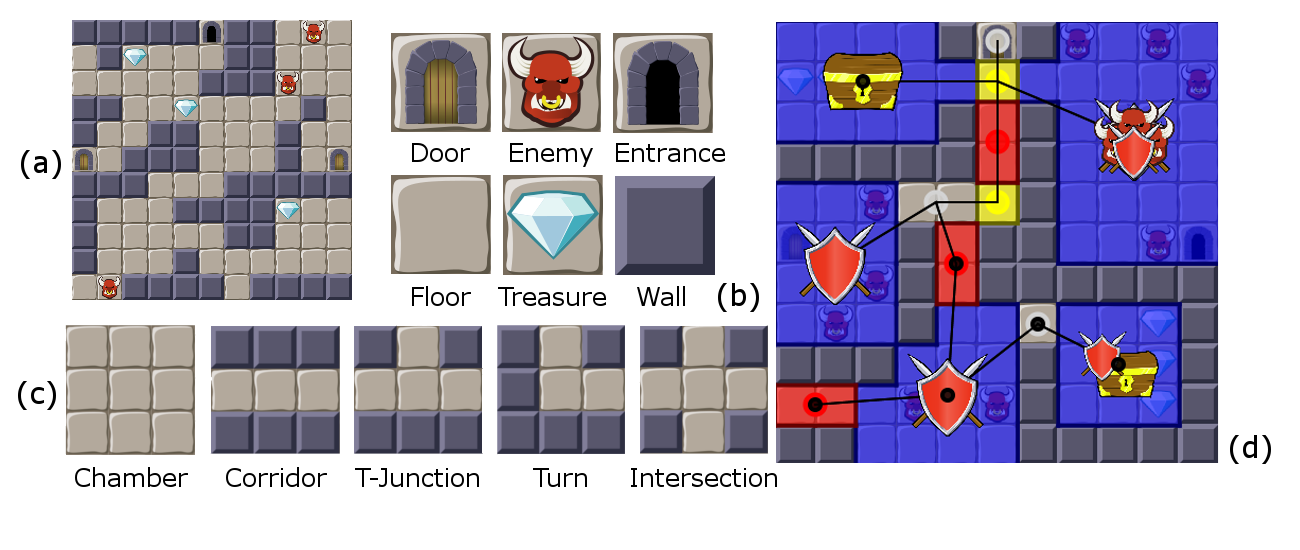
\includegraphics[width=\textwidth]{figure1.png}}
\caption{Main components in EDD. (a) Basic room, (b) different placeable tiles, (c) micro-patterns and (d) meso-patterns~\protect\citepthird{p3Alvarez2018a}.}
\label{figs:basecomponents}
\end{figure}

\begin{figure}[t]
\centerline{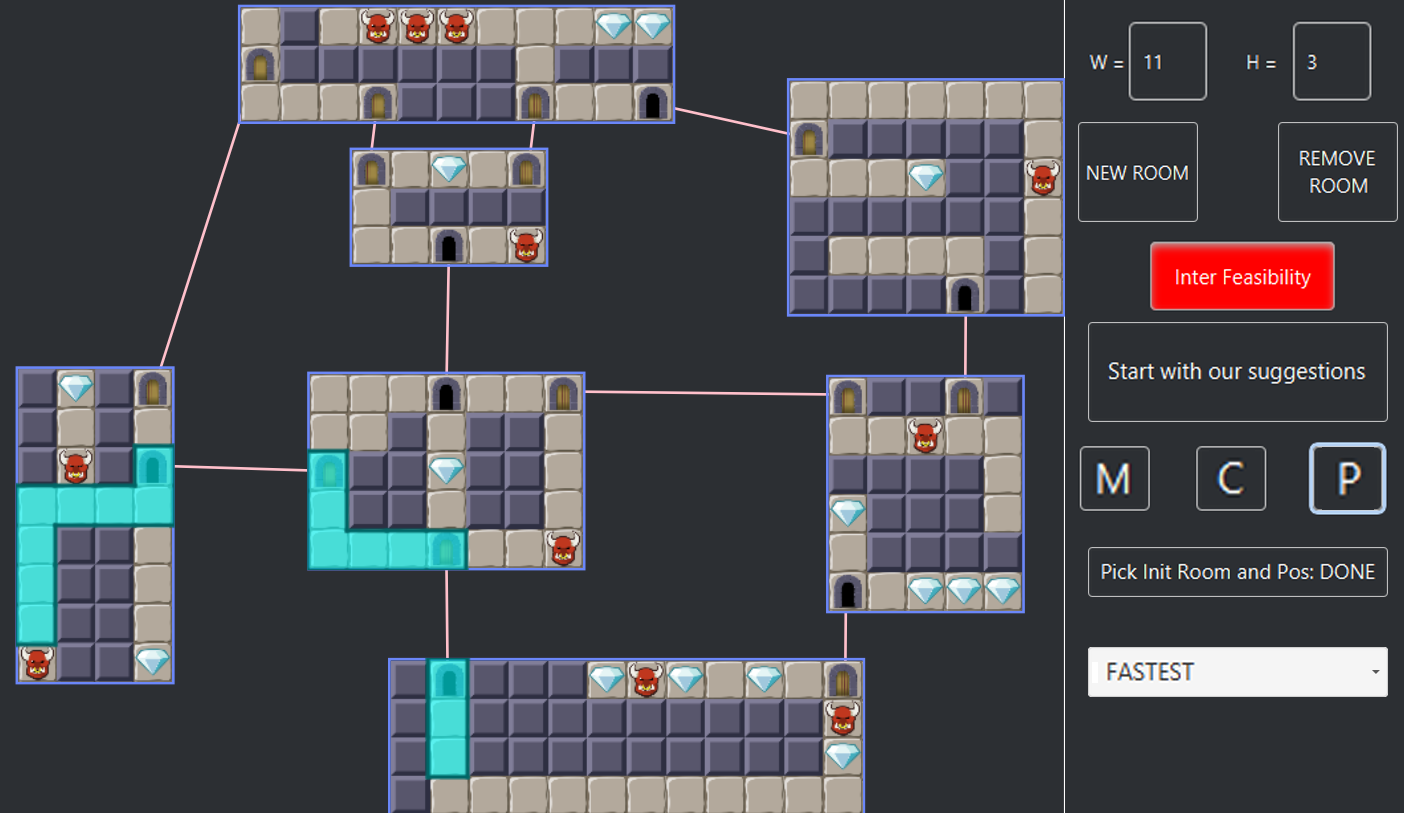
\includegraphics[width=\textwidth]{figure2.png}}
\caption{Screenshot of the dungeon editor screen in EDD, displaying a sample dungeon composed by seven rooms. The shortest path between two given tiles is highlighted in blue. The right pane contains all options for editing the dungeon. "M", "C", and "P" stand for "Move rooms", "Connect rooms", and "calculate Path".}
\label{figs:dungeonscreen}
\end{figure}

\subsubsection{Map-Elites for illuminating search spaces}

Quality-diversity algorithms are algorithms which search a space of solutions not just for the single best solution, but for a set of diverse solutions which are good. MAP-Elites maintains of map of good solutions~\citepthird{p3Mouret2015} and is perhaps the most well-known quality-diversity algorithm. The map is divided into a number of cells according to one or more feature dimensions (commonly, two dimensions are used). In each cell, a single solution is kept. At every update, an offspring is generated based on one or more existing solutions. That offspring is then assigned to a cell based on its feature dimensions, which might or might not be the same as the cell(s) its parent(s) occupy. %If the new offspring has a higher fitness than the existing solution in that cell, it replaces the cell.
If the new offspring has a higher fitness than the existing solution in that cell, it replaces the previous item in the cell. This process results in a map of solutions where each cell contains the best found solution for those particular feature dimensions.

\subsection{Evolving Dungeons as a Whole, Room by Room}

The Evolutionary Dungeon Designer (EDD) is a MI-CC tool that allows a human designer to create a 2D dungeon and its composing rooms (\Cref{figs:basecomponents}.a), being the designer able to manually edit both the dungeon - by placing and removing rooms - and the rooms - by separately editing the tiles (\Cref{figs:basecomponents}.b) that compose each room. EDD's underlying evolutionary algorithm provides procedurally generated suggestions, and is driven through the use of game design micro- and meso- patterns (\Cref{figs:basecomponents}.c and \Cref{figs:basecomponents}.d). A detailed description of all EDD's features can be found in~\citepthird{p3Baldwin2017a,p3Baldwin2017,p3Alvarez2018,p3Alvarez2018a}.

\begin{figure*}[t]
\centerline{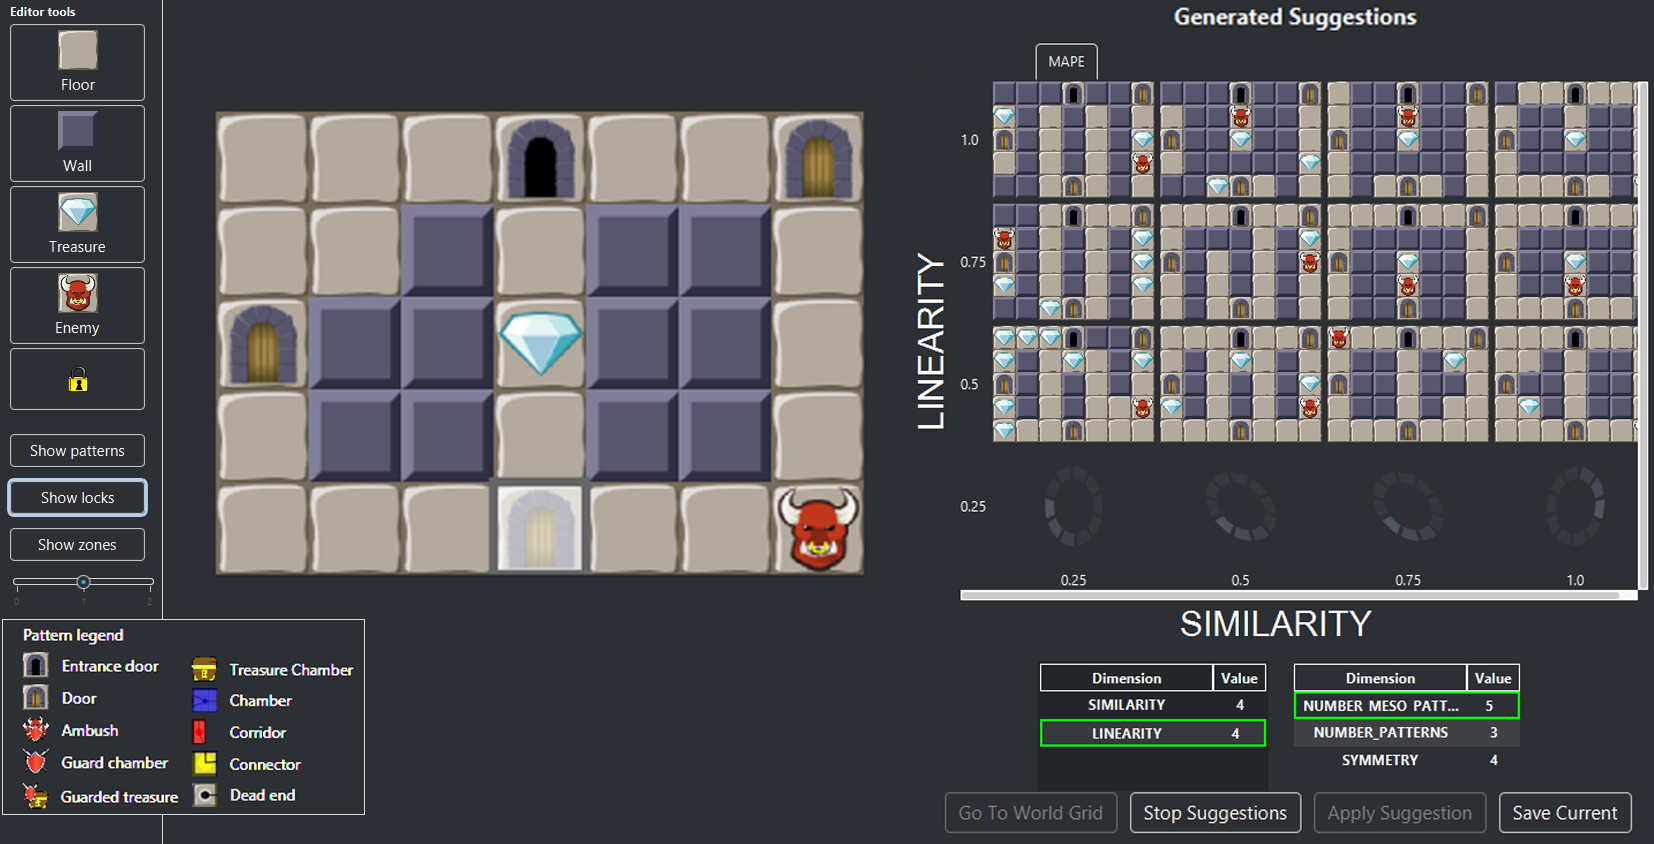
\includegraphics[width=\textwidth]{figure3.png}}
\caption{The room editor screen in EDD. The left pane contains all the options for manually editing the room displayed at the center-left of the screen. The right section displays the procedurally generated suggestions.}
\label{figs:roomscreen}
\end{figure*}

This section presents the latest version of EDD\footnote{available for download at \url{https://drive.google.com/file/d/1lCUfc4OF7lY3vUlPzAqf7i7OUfaKQoem/view}}, which includes significant improvements based on the outcomes from the qualitative analysis discussed in~\citepthird{p3Alvarez2018}. The most significant upgrade is replacing the grid-based backbone that represented the dungeon by a more flexible graph-based representation. A dungeon is now a graph of interconnected rooms of any given size between $3\times3$ and $20\times20$ tiles. The smallest allowed dungeon is composed by two rooms connected once to each other. The designer can perform the following new actions: 

\begin{itemize}
\item adding disconnected rooms to the dungeon. Rooms may also be removed at any time.
\item connecting any pair of rooms by adding a new bi-directional connection to the graph. Rooms interconnect from and to passable border tiles (self-loops are not allowed). Both ends are marked with a door tile (\Cref{figs:basecomponents}.b). A single border tile can only hold one connection, implying that a room can have as many connections as passable border tiles. Connections and rooms can be removed at any time, and their associated doors removed with them.% Removing a room also removes its connections.
\item calculating paths between any pair of passable tiles located in any connected room. Paths are automatically calculated following one the following heuristics: \textit{fastest} returns the shortest path, \textit{rewarding} returns the path that traverses the highest number of treasure tiles, \textit{less danger} provides a path with the fewest number of enemies, whereas \textit{more danger} does the opposite. 
\end{itemize}

The designer is required to select one of the added rooms as the \textit{initial room}, which is the room used by the player to enter the dungeon (for the first time). This selection can be modified unlimited times. The \textit{initial room} is used by EDD to calculate the feasibility of the dungeon. A dungeon is considered feasible when there is at least one path between the \textit{initial room} and any other passable tile in every room. Rooms and doors that aren't reachable from the \textit{initial room} are highlighted in red, so that they can be easily identified by the designer. This feasibility constraint ensures that all passable tiles are accessible, avoiding the possibility of accidentally creating unreachable areas.  

\subsubsection{The mixed-initiative workflow in EDD}

The starting screen in EDD is the dungeon editor screen, shown in \Cref{figs:dungeonscreen}. Every new room is empty (composed solely of floor tiles) when created and is placed detached from the dungeon graph. After manually connecting the room to the dungeon with at least one connection, the designer has the option to populate the room using the room editor screen (\Cref{figs:roomscreen}). This screen can be reached in two different ways:

\begin{enumerate}
\setcounter{enumi}{0}
\item directly: by double-clicking or zooming in (by using the mouse steering wheel or by pinching on the touchpad) on the room. 
\item indirectly: by clicking on the "Start with our suggestions" button on the right pane (\Cref{figs:dungeonscreen}), six procedurally generated suggestions are displayed on a separate screen. The selected suggestion is then opened in the room editor screen. 
\end{enumerate}

\Cref{figs:roomscreen} shows the room editor screen displaying a sample room with the dimensions 7x5 tiles. The left pane lists all the available options for manually editing the room. Manual editing is carried out by brush painting over the room with one of the available tile types: floor, wall, treasure, or enemy. There are two brush sizes (single tile, and five-tile cross shape), and control-clicking allows the designer to bucket paint all adjacent tiles of the same type. Brush painting with the lock button on preserves selected tiles in all the procedurally generated suggestions. A detailed description of all the options in this pane is included in~\citepthird{p3Alvarez2018,p3Alvarez2018a}.

The right side of the screen displays the procedurally generated suggestions, by means of the Interactive Constrained MAP-Elites genetic algorithm (\Cref{section:illuminating}). The "Generate/Stop Suggestions" button at the bottom toggles this algorithm on and off. Once started, the algorithm continuously populates the suggestions pane with new optimal individuals. The evolutionary process is fed with the manually edited room, so that every change in the room affects the generated suggestions. By clicking on "Apply Suggestion", the manually edited room is replaced by the selected suggestion, thus affecting the upcoming procedural suggestions. "Go To World Grid" takes the user back to the dungeon editor screen.

\subsection{Interactive Constrained MAP-Elites\label{section:illuminating}}

%EDD uses a multi-objective fitness function with a FI2Pop genetic algorithm % for EDD, which accounts for two different but related objectives that are associated to the placement and distribution of elements, and the design patterns. The
%where fitness is %thus, 
%a weighted sum divided equally between (1) the inventorial aspect of the rooms, which relates to the placement of enemies and treasures in relation to doors and target ratios, and (2) the spatial distribution of the design patterns, which relates to the distribution between corridors and rooms, and the meso-patterns that those encompass. An in-depth explanation of EDD's fitness function can be found in~\citepthird{p3Alvarez2018a, Baldwin2017}.

%EDD uses a multi-objective fitness function with a FI2PoP genetic algorithm that optimizes (1) the inventorial aspect of the rooms, which relates to the placement of enemies and treasures in relation to doors and target ratios, and (2) the spatial distribution of the design patterns, which relates to the distribution between corridors and rooms, and the meso-patterns that those encompass. Both objectives are combined as a weighted sum divided equally.  An in-depth explanation of EDD's fitness function can be found in~\citepthird{p3Alvarez2018a, Baldwin2017}.

EDD uses a single-objective fitness function with a FI2Pop genetic algorithm where fitness is a weighted sum divided equally between (1) the inventorial aspect of the rooms, which relates to the placement of enemies and treasures in relation to doors and target ratios, and (2) the spatial distribution of the design patterns, which relates to the distribution between corridors and rooms, and the meso-patterns that those encompass. An in-depth explanation of EDD's fitness function can be found in~\citepthird{p3Alvarez2018a,p3Baldwin2017}.

%In addition, 
The overarching goal of MI-CC is to collaborate with the user to produce content, either to optimize (i.e. exploit) their current design towards some goal or to foster (i.e. explore) their creativity by surprising them with diverse proposals. By implementing MAP-Elites~\citepthird{p3Mouret2015} and continuous evolution into EDD, our algorithm can (1) account for the many dimensions that a user can be interested, (2) explore multiple areas of the search space and produce a diverse amount of high-quality suggestions to the user, and (3) still evaluate how interesting and useful the tile distribution is within a specific room. Henceforth, we name the presented approach \textbf{Interactive Constrained MAP-Elites} (IC MAP-Elites). 

\subsubsection{Illuminating Dungeon Populations with MAP-Elites}

MAP-Elites explores the search space more vastly by separating certain interesting dimensions, that affect different aspects of the room such as playability or visual aesthetics, from the fitness function, using them to categorize rooms into niches (cells). %as intrinsic measures of rooms to categorize them into niches (cells). %With such niches, we are able to present diverse suggestions to the user while still maintaining a high quality on them.

\paragraph{Dimensions}

Dimensions in MAP-Elites are identified as those aspects of the individuals that can be calculated in the behavioral space, and that are independent of the fitness calculation. %intrinsic, and more important, independent from the fitness calculation. %, although, as we present in section \Cref{section:results}, the occurrence of individuals in certain dimensional cells correlates with lower or higher fitness scores. 
EDD offers the designer the possibility to choose among the following dimensions, two at a time:
%Currently, we use five different dimensions: (1) symmetry and (2) similarity, related to visual aesthetics, (3) number of meso-patterns and (4) spatial-patterns, related to the presence of patterns in the room, and used to exploit the design pattern characteristics of the room, and (5) linearity, linked to the type of gameplay and possibilities in the room. The user can only choose a pair of dimensions at a time, since presenting higher dimensions would be undesirable and non-understandable for the user. 

\textbf{Symmetry and Similarity.} We choose Symmetry as a consideration of the aesthetic aspects of the edited room since symmetric structures tend to be more visually pleasing. Similarity is used to present the user variations of their design but still preserving their aesthetical edits. Symmetry is evaluated along the X and Y axes, backslash and front slash diagonal and the highest value is used as to how symmetric a room is. Similarity is calculated through comparing tile by tile with the target room. Formulas, information and support for both evaluations are explained in greater details at~\citepthird{p3Alvarez2018a}, where both of them were used as aesthetic fitness evaluations.

\textbf{Number of Meso-patterns.} The number of meso-patterns correlates to the type and amount of encounters the designer wants the user to have in the room in a more ordered manner. The considered patterns are the treasure room (tr), guard rooms (gr), and ambushes (amb). Meso-patterns associate utility to a set of tiles in the room, for instance, a long chamber filled with enemies and treasures could be divided into 2 chambers, the first one with enemies and the second one with treasures so the risk-reward encounter is more understandable for the player. Since we already analyze the rooms for all possible patterns, the number of meso-patterns is simply $\#MesoPat=tr, gr, amb \in AllPatterns$. Equation (\ref{eq:meso-pat-eq}) presents the dimensional value, and since the used meso-patterns can only exist in a chamber, we normalize by the maximum amount of chambers in a room, which are of a minimum size of $3x3$, and results in $Max_{chambers}=\left\lfloor Cols/3 \right\rfloor * \left\lfloor Rows/3 \right\rfloor$.

%All variables will be defined, and such variables names will  be replaced

%\begin{equation} \label{eq:meso-pat-eq}
%D_{mesoPat} = \min{ \left\{     \dfrac{\#MesoPat}{Max_{chambers}}, 1.0}
%\right\} }
%\end{equation}

\begin{equation} \label{eq:meso-pat-eq}
D_{mesoPat} = \min \left\{ \dfrac{\#MesoPat}{Max_{chambers}}, 1.0 \right\}
\end{equation}


\textbf{Number of Spatial-patterns.} By spatial-patterns we mean chambers (c), corridors (cor), connectors (con), and nothing (n). We identify the number of spatial-pattern relates to how individual tiles group (or not) together to form spatial structures in the room. The higher the amount of spatial-patterns the lesser tiles will be group together in favor of more individualism. For instance, a room with one spatial-pattern can be one with no walls and just an open chamber, while a room with a higher number of spatial-patterns would subdivide the space with walls, using tiles for more specific patterns. Equation (\ref{eq:spatial-pat-eq}) presents how we calculate the value for such a dimension. The number of spatial patterns is simply $\#SpatialPat=c, n, cor, con \in AllPatterns$, we then normalize it by the largest side of the room and multiply it by a constant value, determined as $K=4.0$ through a process of experimentation since it resulted in a good estimation of the amount of spatial patterns in the room.

%\textit{not sure of this example} For instance, depicted in figure XXX a., a chamber is a micro-pattern that associate several tiles to one specific pattern, if we then simply add a wall in the middle of it as in figure XXX b., we break the pattern into many other patterns that in turn, create a different type of challenge for the user, a loop. We finally calculate the dimension value with the following formula:

%\begin{equation} 
%\label{eq:spatial-pat-eq}
%D_{spatialPat} = 
%\min{ \left\{ 
%    \frac{\#SpatialPat}{\max\left\{{Cols, Rows}\right\} * \textit{K}}, 1.0}
%\right\}
%\end{equation}

%\begin{equation} 
%\label{eq:spatial-pat-eq2}
%D_{spatialPat} = 
%\min{ \left\{ 
%    \frac{\#SpatialPat}{\max\left\{{Cols, Rows}\right\} * \textit{K}}, 1.0}\right\} }
%\end{equation}

\begin{equation} 
\label{eq:spatial-pat-eq}
D_{spatialPat} = \min\left\{\frac{\#SpatialPat}{\max\left\{{Cols, Rows}\right\} * \textit{K}}, 1.0\right\}
\end{equation}

\textbf{Linearity.} Linearity represents the number of paths that exist between the doors in the room. This relates to the type of gameplay the designer would like the room to have by the distributions of walls among the room. Having high linearity in a room does not need to only be by having a narrow corridor between doors but could also be generated by having all doors in the same open space (i.e. the user would not need to traverse other areas) or by simply disconnecting all paths between doors. Equation (\ref{eq:Linearity-eq}) shows the linearity calculation. Due to the use of patterns, we calculate the paths between doors as the number of paths that exist from a spatial-pattern containing a door to another. Finally, this is normalized by the number of spatial patterns in combination with the number of doors and their possible neighbors.

\begin{equation} \label{eq:Linearity-eq}
D_{lin} = 1 \text{--} \frac{AllPathsBetweenDoors} {\#spatialPat + \#NeighborsPerDoor}
\end{equation}

\paragraph{Continuous Evolution}

%Creation tools are highly dynamic, the user might have an empty canvas in one moment, and after a few interactions over the course of some seconds, they might have a complex room with multiple paths and challenges for the user, and even more ideas on what to do next. Thus, the nature of the tool and the fast-paced interactions require a dynamic and continuous EA that can cope with the requirements of the user and adapt seamlessly to the new changes.

%This interesting paradigm shift, allows the user to focus solely in the design of the rooms while in the background, the EA is adapting to those new designs, rather than waiting for the EA to present suggestions.

EDD implements continuous evolution in two ways. First, the EA constantly updates the target room and configuration with the most recent version of the user’s design, and once the suggestions are broadcasted, that room is incorporated without changes to the population of individuals in the corresponding cell. Secondly, by changing the dimension information and their granularity for the MAP-Elites, which can be done at any given time by the designer. %&in which case, the EA recalculates the cells with the new dimensions and assign the population to the correct cell.% would reset all the cells, calculate their new dimension values and assign the previous populations to the correct cell.

Provided that EDD already uses a FI2Pop, we took as a starting point the constrained MAP-Elites presented by Khalifa et al.~\citepthird{p3Khalifa2018}, where the illuminating capabilities of MAP-Elites explore the search space with the constraints aspects of FI2Pop. This approach manages two different populations within each cell, a feasible and an infeasible one. Individuals move across cells when their dimension values change, or between the feasible and infeasible population according to their fulfillment of the feasibility constraint.

\begin{algorithm}
\footnotesize
\caption{Interactive Constrained MAP-Elites}\label{alg:IC-MAPE}
\begin{algorithmic}[1]
\Procedure{IC-MAP-Elites($\protect[\{d_1,v_1\},...,\{d_n,v_n\}]$)}{}
\State $target \gets curEditRoom$ \Comment{Always in background}
\State createCells$(\protect[\{d_1,v_1\},...,\{d_n,v_n\}])$
\For{$i \gets 1$ to $PopSize$} %\Comment{$PopSize \gets 1000$}
     \State add mutate$(target)$ to $population$
\EndFor
\State CheckAndAssignToCell$(population)$ 
\While {true} \Comment{start continouous evo}
    \For{$generation \gets 1$ to $publishGen$}
        \If {$\textit{dimensionsChanged}$}
            \State $previousPop \gets cells_{pop}$
            \State createCells$(newDimensions)$
            \State checkAndAssignToCell$(previousPop)$ 
        \EndIf
        \MRepeat{ \text{[for feasible \& infeasible pop.]}}
            \For{$i \gets 1$ to $ParentIteration$}
                \State $curCell \gets \text{rndCell}(cells)$
                \State add tournament$(curCell)$ to $parent$
            \EndFor
            \State $offspring \gets  \text{crossover}(Parent)$
            \State checkAndAssignToCell$(offspring)$
        \EndRepeat
        \State sortAndTrim$(cells)$
    \EndFor
    \State broadcastElites() \Comment{render elites}
    \State $pop' \gets cells_{population}$
    \State add mutate$(cells_{pop})$ to $pop'$
    \State add $target$ to $pop'$
    \State checkAndAssignToCell $(pop')$
    \State sortAndTrim$(cells)$
\EndWhile
\EndProcedure
\Procedure{createCells(dimensions)}{}
    \ForEach{$dim \in dimensions $}
        \State add newCell$(dim_d, dim_v)$ to $cells$
    \EndFor
\EndProcedure
\Procedure{$\protect \text{check\&AssignToCell}(curPopulation)$}{}
    \ForEach{$individual \in curPopulation $}
        \State $individual_f \gets evaluate(individual)$ 
        \State $individual_d \gets dim(individual)$
        \State add $individual$ to $cell_{pop}(individual_d)$
    \EndFor
\EndProcedure
\end{algorithmic}
\end{algorithm}

\begin{figure*}[t]
\centerline{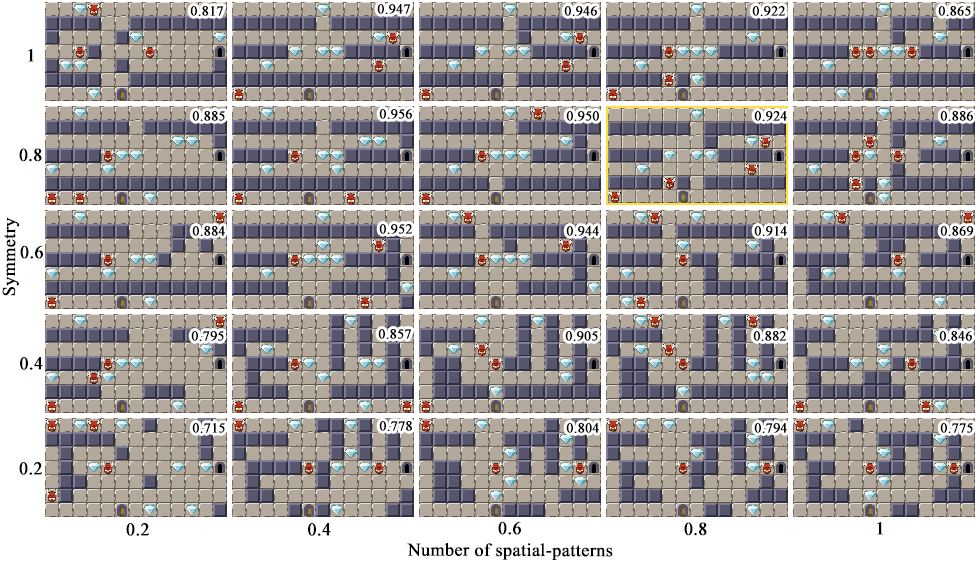
\includegraphics[width=\textwidth]{figure4.png}}
\caption{Rooms at generation $2090$ targeting Number of spatial-patterns (X) and Symmetry (Y). Each cell displays (top-right) the fitness of the optimal individual in its related feasible population. }
\label{figs:patt_sym}
\end{figure*}

\paragraph{Algorithm}

The current evolutionary algorithm is depicted in Algorithm \ref{alg:IC-MAPE}. Cells are first created based on the dimensions selected by the user and proceed to initialize the population based on the user's design, evaluate it and assign each individual to the corresponding cell. Before starting each generation, we check if the dimensions have changed, and if so, recreate the cells and populate them with the previous individuals, and proceed through the evolutionary strategies. Selection is through tournament with a random number of competing parents and offspring are produced through a two-point uniform crossover with a chance of mutation. Offspring are placed in the correct cell and population after calculating their fitness and dimension's information. Finally, cells eliminate the low-performing individuals that over-cap their maximum capacity. Since interbreeding is not allowed, and can only happen indirectly (i.e. the offspring changing population and then used for breeding in consequent generations), the strategies are repeated for each of the population.

This procedure is repeated until the user decides to stop the algorithm. Meanwhile, the EA runs for $n$ generations, and once it reaches the specified limit, it broadcasts the found elites. In order to push the exploration, we first mutate all the individuals from all the populations and cells (while retaining the previous population), and add them into the same pool together with the current edited room without changes. Finally, we evaluate and assign all the individuals to the correct cells, and cells that are over maximum capacity eliminates low-performing individuals.

% Through suggestions based on their design, our EA provides an interesting proposal to the user evaluated with our multi-objective function, which was probably searched in the same exploration space niche as the rest of the population. However, there exist a vast amount of interesting rooms in the search space that are never explored, for instance, having narrow corridors between doors is not the only approach to get high linearity.

% to more interesting and diverse aspects for them. Increasing the granularity of a dimension correlates to the spreading of the already placed individuals into more specific \textbf{change word buckets} “buckets”, and reducing the granularity generalizes more the individuals in such a dimension. %would just mean a lost on expressiveness in order to have more general “buckets”.

% Although such a fitness works well to evaluate the composition of a room functionality-wise based on the design patterns, it falls short for considering all of the different forms of evaluations that a user can have over the provided suggestions.

% While it is crucial that the rooms within the dungeon are playable and feasible, it is not enough to account just for that, as users would like to permeate their rooms with different aesthetics, challenges, paths or even learning aspects. The design of a fitness function that can consider all these different factors and encompasses them into one single value is rather infeasible. The weighted sum of each factor takes away the importance to other aspects, and further aggregating several evaluation dimensions to the fitness function would thus, deepen such a problem.

%\begin{algorithmic}[1]
 % \State this is code \Comment{this is a comment}
%\end{algorithmic}

%\textit{[I think I should have a name for the process of check cell since I keep repeating it and it takes a considerably amount of space]}

\subsection{Experiments}

We ran a set of experiments to test the results from the IC MAP-Elites using all possible combinations of the five available dimensions using two dimensions at a time. All experiments were run using $13\times7$ rooms, the same room size as in \emph{The Binding of Isaac}~\citepthird{p3mcmillen_binding_2011}, a representative example of a dungeon based adventure game.
In each experiment, the initial population was set to $1000$ mutated individuals distributed in feasible and infeasible populations in all cells which were set to a maximum capacity of $25$ individuals each. The EA ran continuously, every $100$ generations rendered the most prominent cells, and at each of the generations, it selected $5$ parents per population among the different cells. Offsprings were produced through a two-point crossover, and were mutated with a 30\% chance.  %The Feasible and infeasible populations in all cells were set to a maximum capacity of $25$ individuals each. 

\nameref{section:results} describes the results achieved and analyzes them in terms of the quality diversity of the suggestions obtained, the existing correlations found between each pair of dimensions, as well as the effects of integrating the MAP-Elites approach into a continuously evolving environment.

\subsection{Results and Discussion\label{section:results}}
\Cref{figs:patt_sym} shows a grid containing the best found suggestions at generation $2090$, while aiming for number of spatial-patterns at the X-axis and symmetry at the Y-axis with a granularity of $5$. Each cell displays the optimal individual of the feasible population under a given pair of dimension values. The fitness score is displayed on the cells' top-right corner.

The fitness evaluation in IC MAP-Elites is quite lightweight in terms of computational cost, so that the grid of suggestions is completed in a matter of seconds. This is of key importance for successfully implementing continuous evolution, so that the influence of each manual change in the edited rooms is reflected in the suggestions almost instantly. The feeling of immediacy is further increased through updating cells as soon as a new optimal individual is produced and incorporated to the cell’s underlying feasible population.

\begin{figure}[ht!]
\centerline{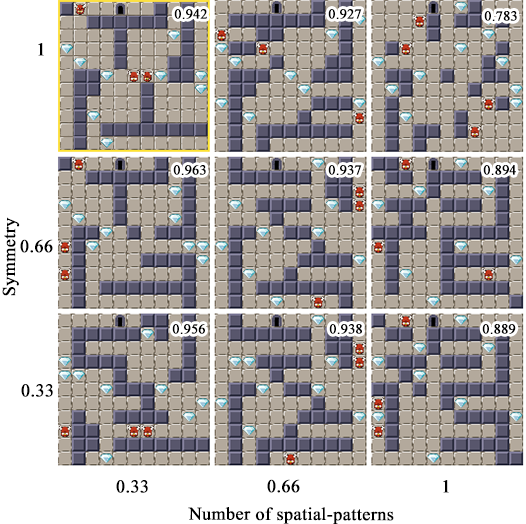
\includegraphics[width=0.6\textwidth]{figure5.png}}
\caption{Rooms at generation $5303$ targeting the same dimensions as in \Cref{figs:patt_sym}, but with the size $11\times11$ instead.}
\label{figs:patt_sym3}
\end{figure}

\begin{figure*}[ht]
\centerline{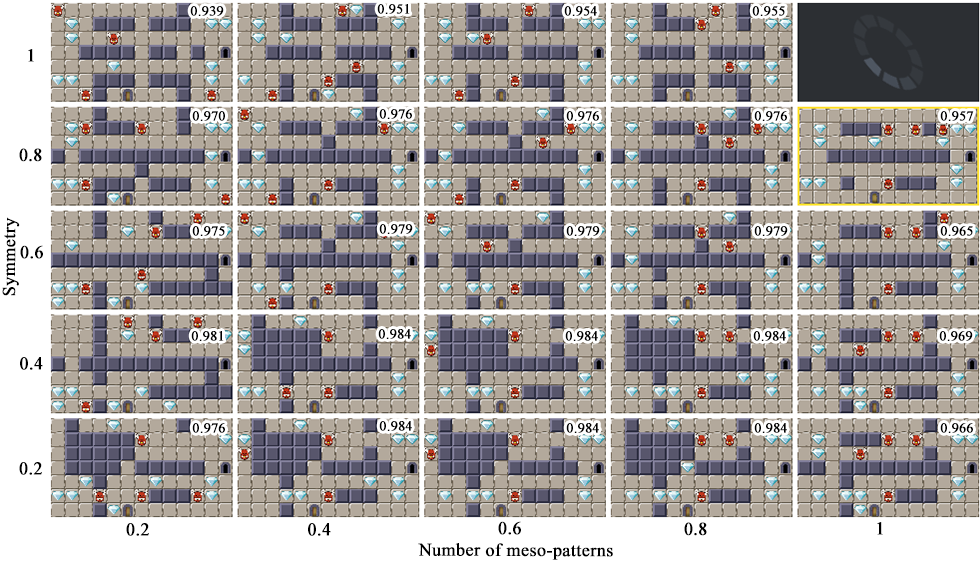
\includegraphics[width=\textwidth]{figure6.png}}
\caption{Rooms at generation $7088$ targeting Number of meso-patterns at the X-axis and Symmetry at the Y-axis. The top-right cell shows that no optimal room could be generated under dimension values $[1,1]$. }
\label{figs:meso_sym}
\end{figure*}

Results in \Cref{figs:patt_sym} are representative of the good quality diversity solutions produced by EDD. The average fitness across cells is $0.872$, and the highest fitness is $0.956$ (cell $[0.4,0.8]$). No two rooms are the same. As intended, high levels of symmetry are displayed in the upper rows, gradually decreasing towards the bottom row. Similarly, rooms in the leftmost column contain lower amounts of spatial patterns, increasing towards the rightmost column. Lower amounts of spatial patterns translate into more open rooms with almost no corridors and one or two large adjacent chambers (as in cell $[0.2, 0.2]$), as opposed to highly pattern filled rooms that comprise intricate pathways converging at one or two small chambers (cell $[1, 0.2]$). Fitness values show that some dimension combinations are harder to optimize than others, so that the whole grid depicts a gradient landscape of the compatibility between each pair of dimensions. 

The bottom-left corner in \Cref{figs:patt_sym} shows difficulties producing symmetric rooms with low amounts of spatial patterns, as opposed to rooms with many corridors (upper-right corner), which seem to favor the generation of symmetrical structures. The bottom row shows that aiming for low symmetry generally produces slightly less optimal results, whereas the top row shows that corridors are the most favorable spatial pattern for building symmetric rectangular rooms. Additional experiments (\Cref{figs:patt_sym3}) show that medium-large square rooms favor the appearance of chambers in combination with corridors for achieving symmetric rooms, thus revealing that squareness and size are important factors for the appearance of chambers in symmetric rooms.

\Cref{figs:meso_sym} contains the rooms generated at generation $7088$ while targeting number of meso-patterns at the X-axis and symmetry at the Y-axis. The top-right cell is empty because its related feasible and infeasible populations are empty, that is, no individuals with value $1$ for both dimensions have been found. The number of empty cells in the earlier generations $3722$, $3875$, and $5864$ were $8$, $7$, and $2$, respectively, indicating that some dimensional values for meso-patterns and symmetry take longer to converge. The continuous nature of IC MAP-Elites fills out the initially empty cells while the designer works with the already generated suggestions. The right half of the grid shows that a combination of small chambers and short corridors favors the appearance of multiple meso-patterns, such as treasure chambers, guarded chambers, and ambushes.

\begin{figure}[ht!]
\centerline{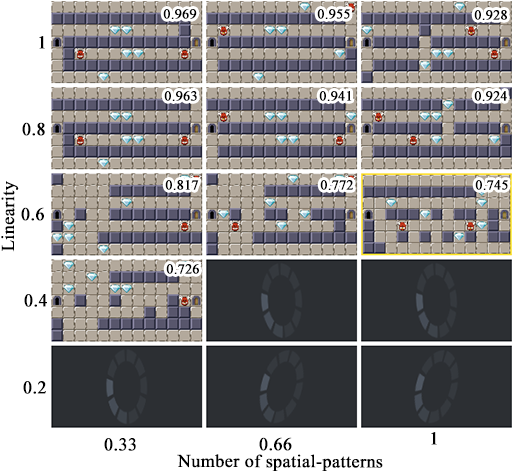
\includegraphics[width=0.6\textwidth]{figure7.png}}
\caption{Rooms at generation $12545$ targeting Number of spatial-patterns at the X-axis and Linearity at the Y-axis.}
\label{figs:lin_patt}
\end{figure}

\begin{figure}[ht!]
\centerline{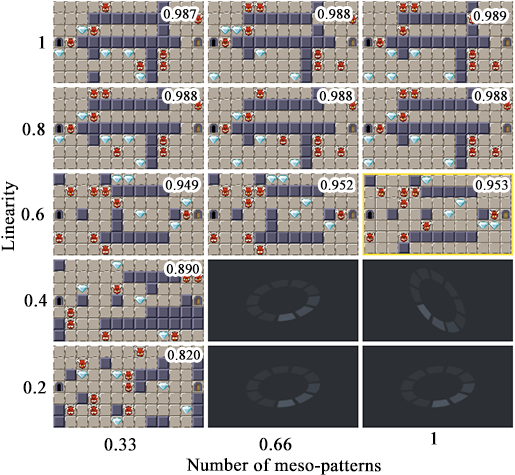
\includegraphics[width=0.6\textwidth]{figure8.png}}
\caption{Rooms at generation $20348$ targeting Number of meso-patterns at the X-axis and Linearity at the Y-axis.}
\label{figs:lin_meso}
\end{figure}

\Cref{figs:lin_patt,figs:lin_meso} show how low valued linearity does not cope well with neither spatial- nor meso-patterns. High linearity tends to create one single pathway, either one long corridor or a wide chamber, that connects the doors in the room. Low linearity results in the opposite, scattering multiple small passages that increase the connectivity between doors but do not count neither as spatial- nor as meso-patterns.

Due to its nature, the performance of similarity in combination with other dimensions has been found to be very dependant on the characteristics already present in the manually edited room. I.e., if this room is already highly symmetric, EDD has problems at preserving similarity while targeting low values of symmetry. This behavior is reported when combining similarity with the other dimensions.

\subsection{Conclusions and Future Work\label{section:conclusion}}
We have presented the Interactive Constrained MAP-Elites, a continuous implementation of MAP-Elites into the Evolutionary Dungeon Designer, creating a MI-CC tool where the users influence the EA through their design, as well as by choosing which dimensions to explore and the granularity of such. 

The presented approach allows the designer to have a fast interaction with the EA through re-targeting and re-scaling the dimensions at will and at any moment. The continuous evolution fits perfectly to the mixed-initiative approach, providing a dynamic search that reacts on the fly to the different interactions of the user, as well as constantly offering new suggestions accordingly. Moreover, mixed-initiative fills the lapses between generations by inviting the designer to permeate the suggestions with custom aesthetics, challenges, paths, and other design decisions. Results show that this approach creates a very fluent workflow of mutual inspiration between designer and tool, yet offering highly customized quality diversity procedural suggestions. 

Results also allowed us to study the compatibility between each pair of dimensions, spotting existing correlations among them and with the fitness function, as well as compatibility pitfalls that leave room for further analysis.

We aim to validate IC MAP-Elites with a user study, as well as to explore alternatives to visualize higher dimensions through the use of CVT-MAP-Elites~\citepthird{p3cvt-mape2016} and Cluster MAP-Elites~\citepthird{p3cluster-mape2017}, analyze the effect of including more dimensions, and performing agent-based dungeon evaluation to improve the fitness calculation by incorporating automatic gameplay data.

\subsection*{Acknowledgement}
The Evolutionary Dungeon Designer is part of the project \textit{The Evolutionary World Designer}, which is supported by The Crafoord Foundation.

\bibliographystylepthird{ieeetr}
\bibliographypthird{included-papers-tex/paper-3/references.bib}

\setcounter{figure}{0}    
\setcounter{table}{0}    
\setcounter{footnote}{0}        

% \clearpage
\graphicspath{{included-papers-tex/paper-4/figures/}}

\includedPaper{\textsc{paper iv - perceived behaviors of personality-driven agents}}{\textsc{paper iv - perceived behaviors of personality-driven agents}}{Alberto Alvarez and Miruna Vozaru}

\normalfont
% \textbf{\textsc{ABSTRACT}}

% We propose modeling designer style in mixed-initiative game content creation tools as archetypical design traces. These design traces are formulated as transitions between design styles; these design styles are in turn found through clustering all intermediate designs along the way to making a complete design. This method is implemented in the Evolutionary Dungeon Designer, a research platform for mixed-initiative systems to create roguelike games. We present results both in the form of design styles for rooms, which can be analyzed to better understand the kind of rooms designed by users, and in the form of archetypical sequences between these rooms. We further discuss how the results here can be used to create style-sensitive suggestions. Such suggestions would allow the system to be one step ahead of the designer, offering suggestions for the next cluster, assuming that the designer will follow one of the archetypical design traces.

\textbf{\textsc{PUBLISHED IN}}

Violence | Perception | Video Games: New Directions in Game Research, [transcript], 2019

%\section*{PERCEIVED BEHAVIORS OF PERSONALITY-DRIVEN AGENTS}

\section*{PERCEIVED BEHAVIORS OF \\ PERSONALITY-DRIVEN AGENTS}

\subsection{Introduction}

The discussion regarding the believability of video game characters in the fields of game analysis and artificial intelligence research has taken many forms over the years, generally focusing on appearance and behavior~\citepfourth{p4Lankoski2007-GameplayDesignPatterns,p4Umarov2012-BelievableAI,p4Lee2012-BelievableCharacters}. In the paper at hand, we will present a study in which we chose to focus on behavioral believability.

The pervading notions related to the degree of character believability seem to be their awareness, reaction capabilities, and adaptability to the events taking place around them~\citepfourth{p4Warpefelt2014-BelievabilityNPC}. These factors seem to be connected to the mental schemas activated by the visual depictions of characters and the game world~\citepfourth{p4Stein92-SchemasCognitiveScience}. This made us question how the believability of an agent would be affected by the absence  of anchoring references. Stripping away referential visual depictions, narrative, and the relevance of affordances to the traversal of the game world, we sought to understand the narratives that observers create around an ambiguous entity acting within an abstract environment.

In this paper, we will first present our reasoning and the theoretical background of the research design, the technical aspects of the AI agent that served as our character, and the responses that participants provided following the viewing of several films depicting the actions of the agent. Finally, we will discuss our conclusions and implications for future research and game development.


\subsection{Theoretical Background}

The purpose of this research is to analyze the means through which the viewer makes sense of ambiguous behavior in the absence of corresponding mental schemas. To do this, we needed to understand the means by which information is perceived and integrated, and what the observer uses to fill in the blanks when the stimulus is too ambiguous to fit into pre-existing information. New information, such as that presented by the behavior of an observed game character, is integrated within the pre-existing mental schemas of the observer, which are used to shape the meaning of the new information and make predictions about future developments. For instance, in the video game PORTAL~\citepfourth{p4portal}, the portal gun activates the mental schemas corresponding to previously encountered guns in video games. Namely that it can shoot, it is a tool for progressing in the game, and it damages enemies. When the portal gun is used, instead of damaging an enemy, it creates a gateway that the player can use to traverse the game. This result does not match pre-existing knowledge, which will force a schema modifi- cation concerning the video game gun functionality. The visual representation affords the integration of the portal gun within the player’s previously acquired knowledge; it is referential, descriptive, and concrete. The differences become apparent once the observed functionality does not match expected performance.
 
Affordance theory, popularized in design by Donald Norman, describes the action and use possibilities that an entity, object, or environment possesses~\citepfourth{p4Norman2002-DesignEverydayThings}. This theory has been widely appropriated by game design, due to the designer’s needs to communicate briefly, clearly, and coherently the means through which a player can traverse a game. Affordances can be tied to previously acquired knowledge, but also be assigned meaning derived strictly from their application within the game world. They are used to telegraph the ways in which the players can use the different elements at their disposal to navigate the game world and to constrain the situational role of the elements.

That being said, the perception of use and role is not a necessary factor in the perception of agency and attribution of specific behaviors. In a study conducted by Heider and Simmel, participants were shown a brief video in which the actors were a circle, a large triangle, and a small triangle~\citepfourth{p4Heider44-ApparentBehavior}. The shapes were depicted in various types of motion, seemingly interacting with each other and the environment. The participants were then prompted to describe the events taking place in the video. All of the participants, with the exception of one, described the events of the video as part of a narrative, whether it was as two parents fighting in front of their child, or two people finding themselves in a romantic situation and then being interrupted by a third. This led us to conclude that the perception of self- directed motion transforms the interpretation of a pattern into one involving an agential entity~\citepfourth{p4Harris2011-AbstractMotion}.

So far, we can conclude that the believability of the agent hinges on its recognizable visual representations, as well as the affordances displayed within the game world. By stripping these factors and endowing a visually ambiguous object with self-directed motion, it will be interpreted as an entity with perceived agency.

Personality traits have generally been viewed as probabilistic determinants for the predictability of a certain type of behavior mediated and moderated by  the current situation~\citepfourth{p4McCrae92-fiveFactorModel,p4Mischel95-TheoryPersonality,p4Tett2000-SituationTrait,p4Costa1998-TraitTheoriesPers}. The Cybernetic Big 5 model, henceforth CB5T, treats personality-endowed agents as goal-based entities perpetually engaged in goal attainment loops~\citepfourth{p4Deyoung2015-CyberBigFive}. The goal loops are divided into stages, with personality traits exerting their influence on each stage of the loop. Traits are manifested through characteristic adaptations, which, unlike personality, are constructed based on individual life experiences and are thus not universal. For instance, the manifestation of the trait compassion can take different characteristic adaptations, such as volunteering or monetary donations, which are dependent on the individual’s socio-cultural environment.

While our intentions steer clear of transforming the research into a projective test\footnote{A projective test is a psychological assessment during which participants are asked to interpret ambiguous stimuli with the assumption that the interpretation will reveal insights regarding their personality traits}, we decided to use personality factors as behavior determinants for our AI agents. Our hypothesis was that in the absence of other anchoring visual primers, the observers would integrate the perceived behavior within familiar characteristic adaptations. While we used Heider and Simmel’s experiment as a starting point, our research was also informed by the similarity-attraction hypothesis, which states that individuals grant more positive appraisals to responses that match their own personality traits~\citepfourth{p4Byrne67-AttractionSimilarity}. The agents were given the same traits as the corresponding observer. We used an AI agent instead of a pre-rendered movie, due to the options it offered in terms of personality customization. We distinguish our purposes from the creation of narratives surrounding ambiguous agents. To clarify, our purpose was not the exploration of the participants’ creation of narratives surrounding the ambiguous behavior of an agent, but to explore the participants’ propensity to recognize behaviors with which they are most familiar – the ones they have observed in themselves.

\subsection{Agent Behavior and Design}

The following section will cover the psychological and visual design of the AI agent, its personality, emotions, and affective behavior, as well as the reasoning behind the aesthetic choices we made.

As mentioned above, the CB5T model moves away from previous models and classifies traits as global influencers of the goal attainment loop, which is broken down into five stages: goal activation, action selection, action, outcome interpretation, and goal comparison. As a result of the ongoing process of receiving, perceiving, and filtering environmental stimuli, multiple goals can be active at the same time. The first and second phases are internal and generally com- prised of parallel processes. The third phase presents a bottleneck to the goal loop, due to the fact that, while a person can hold multiple goals in their memory at the same time, actions are generally performed in sequence. In the fourth phase, the result of the action is measured against the intended results, which  will generate a match or a mismatch. This will in turn inform the next goal and the subsequent cycle. Personality traits exert their influence in concert at every stage of the goal loop, becoming moderators to the goal attainment stages. For a better understanding of the goal loop, we can consider the following situation: The AI agent feels hungry, and in the process of trying to obtain food it realizes that it must jump over an obstacle. While both goals exist in its memory, the fact that it can perform only one action at a time determines that it must first perform the jump. This is the action selection phase. The agent jumps and fails to over- come the obstacle. The actual result and the intended result do not match, and its personality score will influence its reflection on this failure.

The CB5T model was coupled with a simplified version of the  Ortony, Clore, and Collins model of emotions (henceforth OCC), “The OCC model revisited.~\citepfourth{p4Steunebrink2009-OCCModelRevisit}” The reasoning behind the combination of personality and emotion models was derived from the need to visually depict the results of the internal processes taking place during the goal attainment phases. The influence exerted by personality traits on the goal attainment loop materializes in affective behavior, where the emotional valence and intensity is dependent on the personality score.

\begin{figure}[ht!]
\centerline{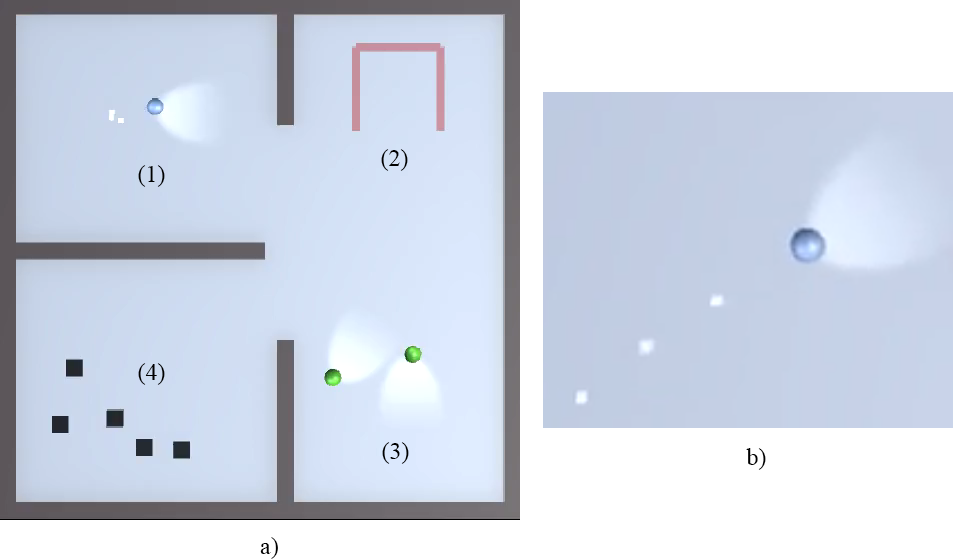
\includegraphics[width=0.8\textwidth]{figure-1-composed.png}}
\caption{Simulation environment.(a) Example environment that was presented to users, containing the personality-driven agent (1), and three different situations that the agent will encounter (2,3,4). (b)	Agent trail and view.}
\label{figs:env-agent}
\end{figure}


Intentionality and attention presented a large part of the concretization of personality-derived behavior. The agent’s attention and intentions were depicted by a cone of light in front of it, maintaining the ambiguity of the stimulus but strengthening the perception of agency. Similarly, the trail the agent leaves be- hind signifies its movement speed which is dependent on its emotional arousal. The affective behavior exhibited by the agent had to be contextualized in specific situations, in order to be granted environmental referentiality. We created several situations, including but not limited to: positive and negative social situations, environmentally challenging situations, and situations that could produce distractions.

\subsection{Agent Architecture and Simulation}

Human-like behavior is a complex subject and one that cannot be approached by using only one model or technique. Rather, different approaches use a compendium of specialized modules. For instance, emotional, personality, memory, or social modules that have various responsibilities in order to simplify the decision-making process.

The TOK architecture represents an agent as a set of different modules that handle the perception, reactivity, goals, emotions, and social behaviors. TOK is divided into three main components: (1) HAP, the goal-based reactive engine, (2) EM, the emotional model, and (3) Glinda, the natural language system~\citepfourth{p4Bates94-architectureAES}.

\begin{figure}[ht!]
\centerline{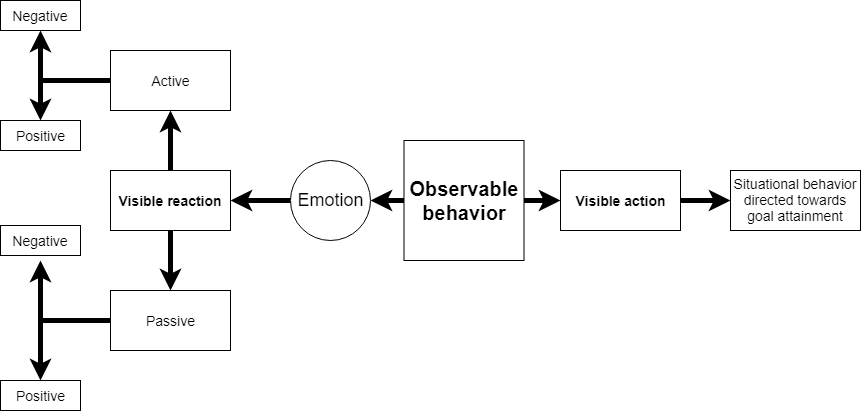
\includegraphics[width=\textwidth]{big-figure.png}}
\caption{Observable Behavior. The observable behavior by the users is based on the set of actions provided by the encountered situation, which results in an emotional reaction. The reaction is based on the outcome interpretation phase, where the agent will choose the respective emotion (active/passive and negative/positive), intensity and reactive behavior.}
\label{figs:observableBehavior}
\end{figure}

Our model assimilates to HAP and EM, in that HAP selects an action based primarily on the agent’s goals, emotions and perception by using the CB5T model, and with EM it calculates the emotional valence of the agent by comparing environmental stimuli with goals, possible actions with standards, and environmental objects with attitudes.

The agent’s goals have a dynamic weight and a priority. The weight is determined by the agent’s moment-to-moment actions and reflect its progression and perception of environmental cues. The priorities indicate the goal type, and their influence on survival and self-actualization. To exemplify, “hunger” is a priority 1 goal, and its weight will increase according to the presence of food in the agent’s proximity and the time they spend roaming around the environment.

Subsequently, according to the outcome of the situation, the agent will feel pleased or displeased in accordance with the match or mismatch between the desired outcome and the actual one. The combination of the outcome difference and the personality traits trigger different emotional reactions. As presented in figure~\ref{figs:observableBehavior}, the agent can perform several actions in specific situations and the con- sequence of the selected action entails not only different emotions but also different levels of arousal.

\newcolumntype{Y}{>{\centering\arraybackslash}X}
\begin{table*}[ht]
% \centering
\caption{Reaction table used to choose the respective emotional reaction. First, we choose the agent’s emotion by choosing if active/passive and negative/positive  as presented in figure 2, with the addendum that if more than one option is viable, the choice will be based on the situation’s target. Finally, the intensity is calculated.} \label{p4tab:reactionTab}
% \resizebox{0.8\textwidth}{!}{
\centering
\begin{tabularx}{0.9\textwidth}{|c|c|Y|}
\hline
Situation type& Event type&	Agent type \\ \hline
Negative/Positive & Displeased/pleased & Standards \\ \hline
Passive/Active & Neuroticism & Neuroticism \\ \hline
LOW/MID/ HIGH & Goal weight & Neuroticism level \\ \hline
Inner choice & Situation target & Situation target \\ \hline
\end{tabularx}
% }
\end{table*}

The way in which different emotional reactions occur was modelled in a table which is live queried to extract the agent’s reaction. Table 1 illustrates how a reaction is chosen based on the two types of situations presented in our simulation.

\subsection{Simulation}

In order to control the agent’s decisions, we built a decision tree that uses personality traits, perceived situations, and the current goal weight as inputs. The decision tree allows the agent to acquire its next goal, perform the action, and exhibit the corresponding emotional reaction. Therefore, the decision tree has five steps: (1) sense the environment, (2) reason about the possible actions based on their goals, (3) engage with the situation, (4) reflect on the outcome, and (5) produce an emotional reaction.

The agent constantly senses its surroundings to gather encountered entities, it inventories the situations they generate and compares them to its inner goals, and then chooses the situation that would satisfy the primary goal. To simulate the attraction towards novelty, every situation the agent engages in becomes less novel every time it is chosen. Once a specific type of situation becomes ordinary (i.e. not novel), the agent will give more weight to other types of situations.

Each situation has its own set of afforded behaviors. For instance, in a situation in which the agent can encounter other agents, it can approach them, give objects to them, or perform other context-specific actions. This allowed us to simplify the agent’s decision-making step by allocating complexity to each situation.

Situations are divided into two main categories: environmental challenges and social challenges. For instance, the agent might \textbf{encounter an obstacle}, and finding out what is on the other side of it will satisfy its curiosity goal. Or it might engage in a situation where other agents are \textbf{having fun}, which in turn would satisfy the \textbf{social acceptance goal}.

Although the agent is given a set of behaviors to perform, there are cases where the agent will simply not perform the action, due to not having the necessary resources, being physically unable to do it, or due to a conflict with its personality traits. For instance, the agent might not be able to give any object to collecting agents, as the agent has not found anything yet, or to jump a gap due to low levels of assertiveness and high withdrawal.

Once the situation has been resolved, the agent compares the actual outcome to the expected one and the respective weight is modified accordingly. This final step triggers the agent’s emotional reaction, defined by the Figure 2 process and reached by the queried information from the reaction table (Table 1). Finally, the agent goes back to its ordinary state and repeats the goal attainment loop.

\subsection{Participant Assessments and Responses}

Participants were selected using a snowball method. Both the selection method and the low number of participants (n=6) preclude us from generalizing results. Participants were informed that they would take part in a study focusing on behavior perception in a virtual environment. In the first stage of the research, the participants were asked to fill out a personality evaluation questionnaire. The questionnaire was comprised of 50 items, taken from the International Item Pool, and tailored to the CB5T~\citepfourth{p4goldberg2006-personalityItemPool}.

The scores were subsequently calculated and assigned to an individual agent. The agents were placed in the same environment and recorded while acting within the given environment. Consequently, the recordings were shown to the participants, who were asked to describe the behavior of the agent and what they thought the actions represented, without being aware of the specific traits given to the agent.

While the small number of participants does not allow us to draw generalizable conclusions, the responses indicate the recognition of the agent as an entity with directed behavior and agency, to which they attributed familiar characteristic adaptations. One of the participants described their agent’s behavior as follows:

\begin{retQuestion}{}
   “(…) the agent is similar to a person that works in an office. He is engaging in conversation with his co-workers/superiors and tries to do his day-to-day tasks. As I see it, the agent has a lot of work to do, as he is in a continuous movement. I think he should take a break from time to time.”
\end{retQuestion}

We can see that the ambiguous movement of the agent is identified with a specific characteristic adaptation, and the environment is given characteristics that e replace abstract representations with imagery from an everyday office space. The participant also evaluates the agent in a sympathetic manner, which we can consider a byproduct of the contextualization within a familiar characteristic adaptation.

A different participant, viewing the behavior of their own agent in the same environment, described the behavior as follows:

\begin{retQuestion}{}
    “He’s pretty anxious, he isn’t sure of himself, of what he’s going to do (with the box). At first he seemed a bit shy, he basically wanted to avoid the other two, and I think he didn’t even say hello to them (...)”
\end{retQuestion}


We can see that the agent’s movements of approach and withdrawal are described here through the lens of common human social behavior of greeting and social avoidance. The agent is also given specific, human-like traits, which signal recognition and contextualization of behavior.

The responses also reflect drawbacks in our aesthetic choices, but strengthen the hypothesis that, when confronted with ambiguous cues, the participants will appeal to their most readily available mental schema. One participant wrote:

\begin{retQuestion}{}
   “This agent looks like it’s sweeping the ground for something with a metal detector. It checks both sides of the box but looks like it doesn’t find anything.”
\end{retQuestion}

While the cone of light was intended to be a signifier of attention and intention, it was interpreted in this case as a concrete object, a metal detector. However, the participant’s interpretation that grounds the agent’s behavior as exploratory is consistent with our hypothesis of the need to concretize ambiguous behaviors.

We can see the ways in which the participants interpret, and ascribe meaning to, the ambiguous behaviors of the agent. While remaining in the realm of the abstract, the motions and actors could be described as “the dot got closer to the other dots and then got further away.” However, the participants attributed emotion and reasoning to the entity.

\subsection{Conclusion}

This pilot experiment explored the ways in which people attribute known and familiar behaviors to an AI agent in the absence of other anchoring visual cues. Participants who, unknowingly at the time, contributed to the creation of the AI by providing data regarding their personality traits, largely interpreted ambiguous behavior by association with their own characteristic adaptations. Future research into this area could explore the interpretation of behavior exhibited by AI agents that have different personality traits than those of the observers. While stripping visual cues from the environment and characters is not a valid aesthetic choice for most video games, the central take-away of this experiment should be the importance of missing information, whether deliberate or not.

The behavior descriptions reflect the participant’s propensity for filling in blanks with their own familiar characteristic adaptations. When presented with merely a few rectangles and spheres, one participant saw an office, while another saw a social situation that the protagonist was trying to avoid. These results point to an important value that should be considered in the design, critique, and analysis of digital games: the ambiguity variable.

One of the key missing pieces of this research was the capability of the participants to execute actions within the environment. This would have given the agent in-world affordances, allowing the players to integrate their own intentionality and project their characteristic adaptations onto the performed actions. However, at this stage we did not want to assess the participants’ projection of personal actions, but rather their perception of ambiguous events and characters.

Our agent was a capsule, a dot on a two-dimensional plain. However, motion granted it the status of an entity and its ambiguous actions afforded it reasoning, motives, and personality (in the eyes of the participants). The participants were not aware of the personality traits that the agent had been given, but they were able to recognize the narrative around them. The results of the research underline that when ambiguity is present, the space will be filled by the viewer’s characteristic adaptations. This research is just a pilot, and drawbacks such as the limited number of participants and lack of interactivity should be addressed in future iterations.

\subsection{Acknowledgement}

Miruna Vozaru ackowledges the financial support received from the European Research Council (ERC) under the European Union’s H2020 ERC-ADG program (grant agreement No 695528)

\bibliographystylepfourth{ieeetr}
\bibliographypfourth{included-papers-tex/paper-4/references.bib}

\setcounter{figure}{0}    
\setcounter{table}{0}    
\setcounter{footnote}{0}      

% \clearpage
\graphicspath{{included-papers-tex/paper-5/figures/}}

\includedPaper{\textsc{paper v - learning the designer's preferences to drive evolution}}{\textsc{paper v - learning the designer's preferences to drive evolution}}{Alberto Alvarez and Jose Font}

\normalfont
\textbf{\textsc{ABSTRACT}}

This paper presents the Designer Preference Model, a data-driven solution that pursues to learn from user generated data in a Quality-Diversity Mixed-Initiative Co-Creativity (QD MI-CC) tool, with the aims of modelling the user's design style to better assess the tool's procedurally generated content with respect to that user's preferences. Through this approach, we aim for increasing the user's agency over the generated content in a way that neither stalls the user-tool reciprocal stimuli loop nor fatigues the user with periodical suggestion handpicking. We describe the details of this novel solution, as well as its implementation in the MI-CC tool the Evolutionary Dungeon Designer. We present and discuss our findings out of the initial tests carried out, spotting the open challenges for this combined line of research that integrates MI-CC with Procedural Content Generation through Machine Learning.

\textbf{\textsc{PUBLISHED IN}}

Proceedings of the 23rd European Conference on the Applications of Evolutionary and bio-inspired Computation, EvoApplications '20, Springer, 2020

\section*{LEARNING THE DESIGNER'S PREFERENCES TO DRIVE EVOLUTION}

\subsection{Introduction}

As game production grows, so does the usage of computer-aided design (CAD) tools to develop various facets of games. CAD tools enable users to create new content or refine previously created content with the assistance of some type of technology that focuses on reducing the workload of the developer. Procedural Content Generation (PCG) denotes the use of algorithms to generate different types of game content, such as levels, narrative, visuals, or even game rules, with limited human input \citepfifth{p5shaker_procedural_2016}. Search-based PCG is the subset of techniques whose approach generates content by using a search algorithm, a content representation mechanism, and a set of evaluation functions to drive the content creation process towards near-optimal solutions \citepfifth{p5Yannakakis2018}. 

Mixed-initiative co-creativity (MI-CC)~\citepfifth{p5yannakakis2014micc} is a branch of PCG through which a computer and a human user create content by engaging into an iterative reciprocal stimuli loop~\citepfifth{p5shaker2013ropossum,p5smith_tanagra:_2011,p5machado2019pitako,p5liapis_generating_2013,p5guzdial-lvldsg-aiide-2018,p5lucas-3buddy-iccc2017}. This approach addresses the design process with insight and understanding of the affordances and constraints of the human process for creating and designing games \citepfifth{p5Liapis2016}. MI-CC helps designers to either optimize their current design towards a specific goal (thus exploiting the search space) or foster their creativity by proposing unexpected suggestions (exploring the search space). To these ends, diversity has been an important feature for the research community to focus on during the past decade, including novelty search~\citepfifth{p5Novelty-Lehman2011}, surprise~\citepfifth{p5Surprise-Gravina2016}, curiosity~\citepfifth{p5CuriositySearch-Stanton} and, more recently, quality-diversity approaches \citepfifth{p5Khalifa2018}. 

PCG through Quality-Diversity (PCG-QD) \citepfifth{p5gravina2019procedural} is a subset of search-based PCG, which uses quality-diversity algorithms~\citepfifth{p5Pugh2016} to explore the search space and produce high quality and diverse suggestions. MAP-Elites \citepfifth{p5Mouret2015} is a successful quality-diversity algorithm that maintains a map of good suggestions distributed along several feature dimensions. A constrained MAP-Elites implementation was presented by Khalifa et al.~\citepfifth{p5Khalifa2018}, combining MAP-Elites with a feasible-infeasible (FI2Pop) genetic algorithm~\citepfifth{p5Kimbrough2008} for the procedural generation of levels for bullet hell games. The first implementation of a PCG-QD algorithm for MI-CC was presented by Alvarez et al. \citepfifth{p5alvarez2019empowering}, elaborating on the combined MAP-Elites and FI2Pop approach by introducing a continuous evolution process that benefits from the multidimensional discretization of the search space performed in MAP-Elites.

In all the above MI-CC approaches, the designers play an active role in the procedurally generated content while struggling between the expressiveness of the automatic generation and the control that they want to exert over it \citepfifth{p5Alvarez2018}. Having this as motivation, this paper takes the work in \citepfifth{p5alvarez2019empowering} one step forward by adding an underlying interactive PCG via machine learning algorithm \citepfifth{p5summerville2018procedural}, the Designer Preference Model, that models the user's design style, to be able to predict future designer's choices and thus, driving the content generation with a combination of the designer's subjectivity and the search for quality-diverse content.

% , which have been concluded in several studies [ref]. 

% [ref to picbreeder, novelty search picking paper, spaceship generation]. 


\subsection{Previous work}

\subsubsection{Mixed-Initiative Co-Creativity}
Similar to user or player modeling, designer modeling for content creation tools (CAD and MI-CC tools) was suggested by Liapis et al~\citepfifth{p5Liapis2013-designerModel}, where it is proposed the use of designers models that capture their styles, preferences, goals, intentions, and interaction processes. In their work, they suggest methods, indications, and advice on how each part can be model to be integrated into a holistic designer model, and how each game facet can use and benefit from designer modeling. Moreover, in \citepfifth{p5Liapis2014-designerModelImpl} the same authors discuss their implementation of designer modeling and the challenges of integrating all together in their MI-CC tool, Sentient Sketchbook, which had a positive outcome on the adaptation of the tool towards individual “artificial” users.

Furthermore, Lehman et al \citepfifth{p5lehman2016creative} presented Innovation Engines that combine the capabilities and advantages of machine learning and evolutionary algorithms to produce novel 3D graphics with the use of Compositional Pattern-Producing Networks (CPPN) evolved with MAP-Elites, and evaluated by the confidence a deep neural network had on the models belonging to a specific object category.

\subsubsection{Procedural Content Generation via Machine Learning}
Summerville et al. \citepfifth{p5summerville2018procedural} define Procedural Content Generation via Machine Learning (PCGML) as the generation of game content by models that have been trained on existing game content. The main approaches to PCGML are: autonomous content generation, content repair, content critique, data compression, and mixed-initiative design.

\begin{figure}
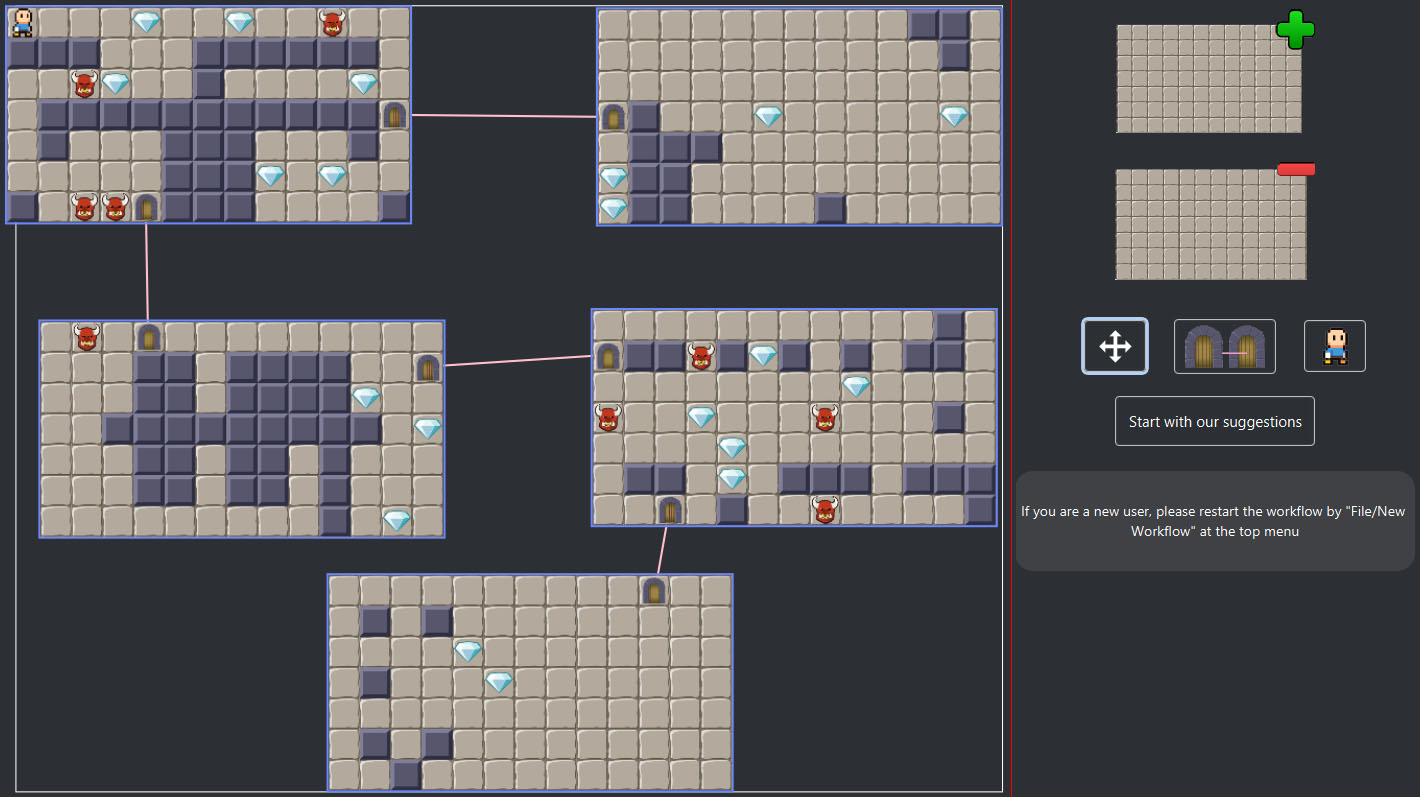
\includegraphics[width=\textwidth]{fig1.jpg}
\caption{Screenshot of the dungeon editor screen in EDD, displaying a sample dungeon composed by five rooms.} \label{p5fig1}
\end{figure}

In the latter case and, as appointed by Treanor et al. \citepfifth{p5treanor2015ai}, AI may engage with a human user participating in the creation of content, so that new gameplay emerges from this shared construction. This emerging relationship between the user and the AI system, when implemented through a trained machine learning algorithm, has the potential to reduce user frustration, error, and training time. This is due to the capacity of a machine learning solution to adapt to the design preferences of the user that interacts with the MI-CC tool by learning from the user-generated dataset of previous choices.

\subsubsection{The Evolutionary Dungeon Designer}

The Evolutionary Dungeon Designer (EDD) is an MI-CC tool for designers to build 2D dungeons. EDD allows designers to manually edit the overall dungeon and its composing rooms (see Figure \ref{p5fig1}), as well as to use procedurally generated suggestions either as inspiration to work on or as a finished design (see Figure \ref{p5fig2}). Both options fluently alternate during the creation process by means of a workflow of mutual inspiration, through which all manual editions performed by the user are fed into the underlying continuous Evolutionary Algorithm, accommodating them into the procedural suggestions. A detailed description of EDD and its features can be found in~\citepfifth{p5Alvarez2018a,p5Alvarez2018,p5Baldwin2017a,p5Baldwin2017}.

Subsequent user studies \citepfifth{p5Alvarez2018,p5Baldwin2017} carried out with game designers on EDD raised the following areas of improvement: (1) the designers struggled with EDD’s capability of understanding the designer’s intentions and preserving custom designs; (2) the tool was unable to generate aesthetically pleasing suggestions since the fitness function only accounted for functionality, but not aesthetics, of design patterns; (3) the designers wanted to keep certain manual editions from being altered by the procedural suggestions.  

With the aims of addressing these limitations as well as fostering the user's creativity with quality-diverse proposals, EDD was improved with the Interactive Constrained MAP-Elites (IC MAP-Elites) \citepfifth{p5alvarez2019empowering}, an implementation of MAP-Elites into the continuous evolutionary process in EDD. With this addition, the user drives the generation of procedural suggestions by modifying at any moment the areas of the search space where the evolution should put the focus on. This is done by selecting among the available dimensions: symmetry, similarity, design patterns, linearity, and leniency. Additionally, the designers have now the chance to limit the search space by locking map areas and thus preserving manually edited content.

This paper contributes by building on top of EDD's IC MAP-Elites, adding a data-driven Designer Preference Model that adapts and personalizes the design experience, as well as balances the expressivity of the tool and the controllability of the designer over the tool. Other researchers have pursued a similar goal by biasing the search space through having the user perform a manual selection after every given number of generations~\citepfifth{p5Picbreeder-Secretan2008,p5Liapis2012-adaptiveVisual,p5Novelty-Lehman2011}. Nevertheless, this approach leads to an increase in user fatigue by repeatedly asking for user input and thus, stalling the evolutionary process until such input is received. Moreover, this staged process seems incompatible with the dynamic reciprocal workflow of MI-CC tools, where the focus is on the designer proactively creating content rather than passively browsing a set of suggestions.

\begin{figure}[t]
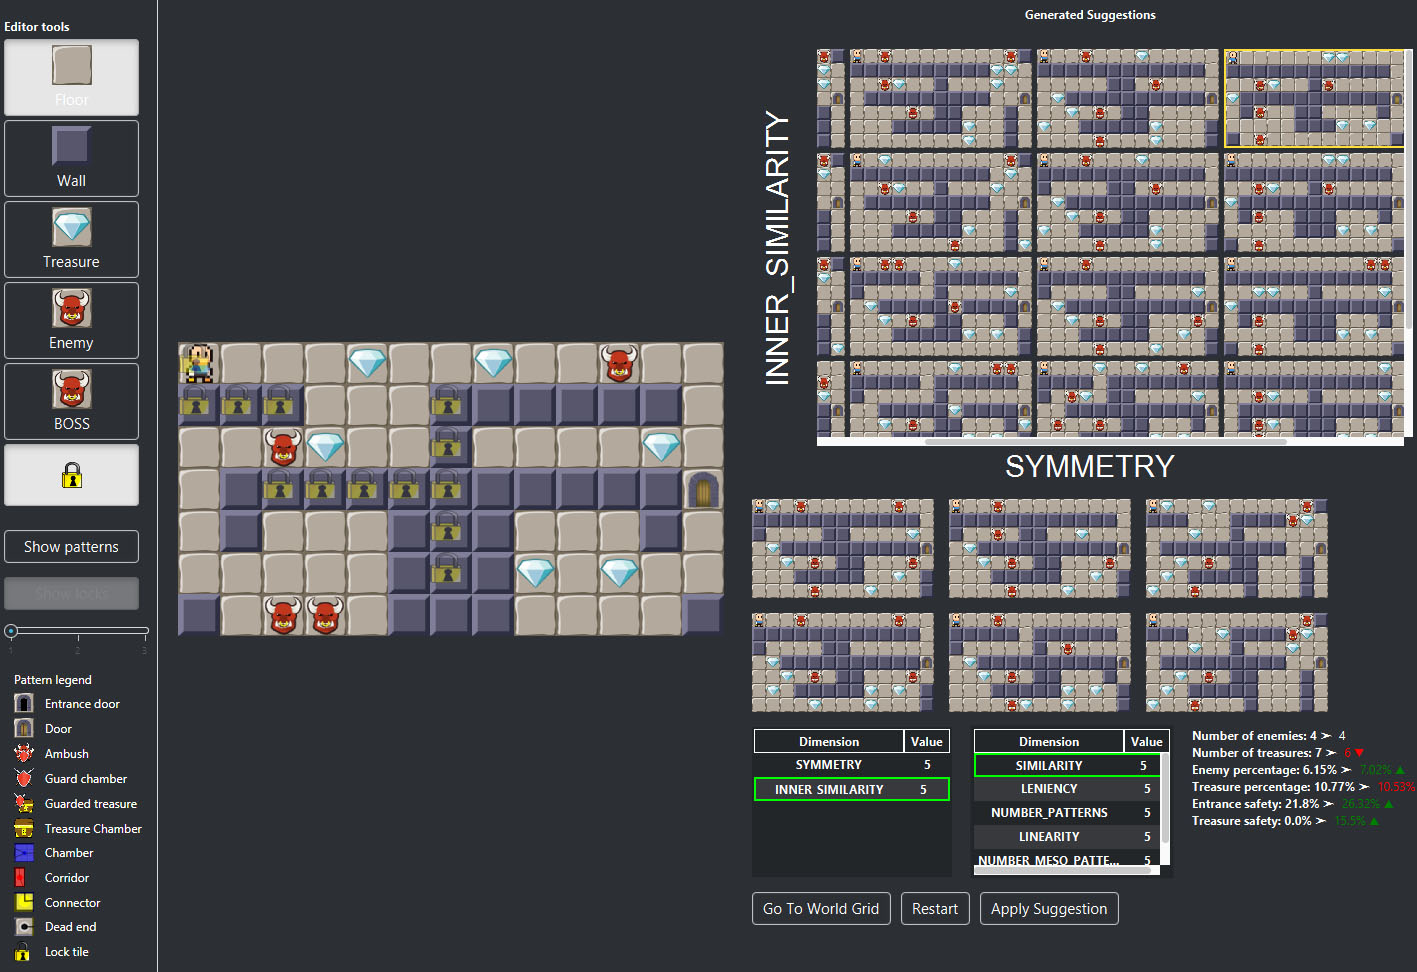
\includegraphics[width=\textwidth]{fig2.jpg}
\caption{The room editor screen in EDD. The top-right pane shows the suggestions provided by the IC MAP-Elites algorithm. Below are the six top-raked suggestions by the Designer Preference Model. The left pane contains the manual edition features.} \label{p5fig2}
\end{figure}

The remaining sections of the paper are structured as follows: Section 3 describes the data-driven Designer Preference Model; Section 4 presents the initial experimental results, and Section 5 discusses the results and future lines of research of this novel approach.

%%Check the section references!
\subsection{Designer Preference Model} \label{p5section/model}

The Designer Preference Model is a data-driven intelligent system that learns the user's design style by training and testing over a continuously growing dataset composed of the user's actions and choices while operating EDD. The underlying evolutionary algorithm (EA) uses this model to assess the generated suggestions according to the predicted preference of the designer. This is a complementary assessment to EDD's original fitness function, which evaluates individuals first based on the presence and distribution of spatial and meso-patterns (Figure \ref{p5fig3}), and then based on their degree of adaptation to the user-selected quality-diversity dimensions \citepfifth{p5alvarez2019empowering}. The relevance of the Designer Preference Model gradually increases over EDD's fitness function as long as the model gains confidence in its assessments.

\begin{figure}
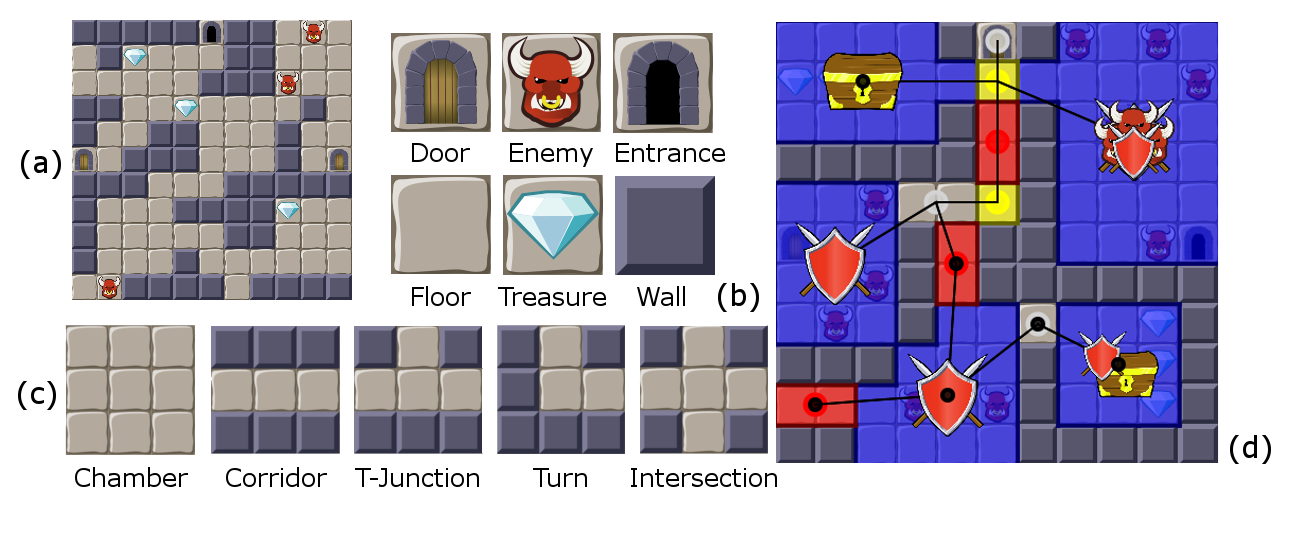
\includegraphics[width=\textwidth]{fig3.png}
\caption{A sample room in EDD (a) compose by tiles (b), spatial patterns (c) and meso-patterns (d). Detailed descriptions for these components can be found in~\protect\citepfifth{p5Baldwin2017a}.} \label{p5fig3}
\end{figure}

\begin{figure}
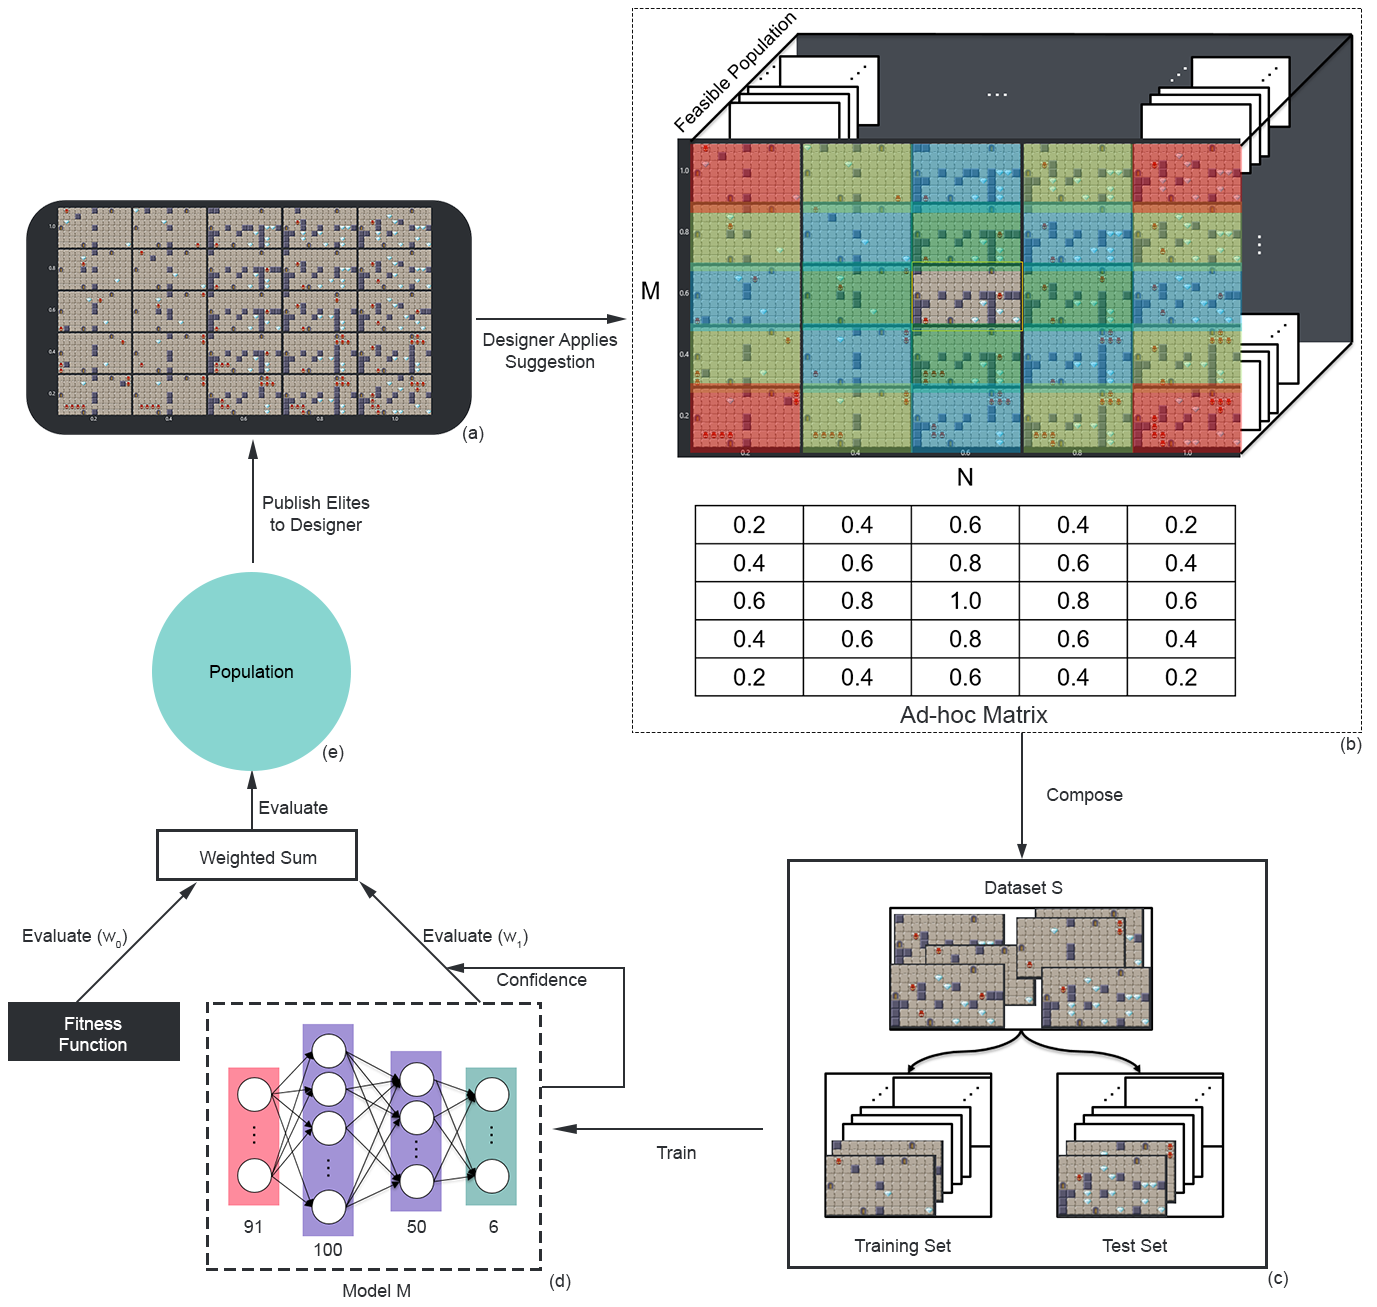
\includegraphics[width=\textwidth]{fig4.png}
\caption{Overview of the Designer Preference Model integrated into the fitness function of EDD. Elites are published and shown to the designer in a grid fashion (a), and once the designer chooses and applies one of the suggestions, an ad-hoc matrix is created based on the position of the selected suggestion to estimate the preference of suggestions (b). The ad-hoc matrix is then applied to all the elites in the grid, and the feasible populations within the EA cells to compose a general dataset $S$ with rooms labeled by the estimated preference. The composed dataset $S$ is then subdivided into a training set (90\%) and test set (10\%), both with the same label distribution (c). The dataset is used to train a model $M$, which is a relatively small neural network, for 20 epochs (d). The  model is then used to evaluate the population of the EA together with the current fitness function in a weighted sum, with the weight of the model $M$ conditioned by the confidence of the network (e).} \label{p5fig4}
\end{figure}

\subsubsection{Model Update and Usage}
The proposed model is a relatively small neural network $M$ with as many input neurons as the number of tiles composing each room, two hidden layers (100 and 50 neurons respectively), and six output neurons, one per each discrete preference value assigned to the individuals by the designer. When the designer starts EDD, the neural network is created with random initialization and without any prior training (i.e. cold start). While the designer creates and modifies rooms, on the background, the EA produces and presents individuals to the designer using the MAP-Elite’s cells (Figure \ref{p5fig2}), while it adapts to the designer’s design. Following a proactive learning approach \citepfifth{p5donmez2008proactive}, anytime the designer chooses one suggestion to replace her current design, a training session is requested for a model $M$ with a dataset $S$ created with the current cells and their populations based on the designer’s chosen suggestion. The loop, depicted in figure \ref{p5fig4}, can be described in the following two steps:

\paragraph{Dataset creation:}

The designer chooses a suggestion to replace her current design, which in turn, requests a training session using all the current individuals (i.e. the elites and the rest of the feasible populations) to create a new dataset to train the model closer to the “actual” preference of the designer. As shown in figure \ref{p5fig4}.b, an ad-hoc matrix is created, based on the position of the applied suggestion, to calculate the estimated preference, starting with the applied suggestion (1.0 preference value), and reducing the preference value by 0.2 per each step that was taken away from the applied suggestion in the matrix until a minimum of 0.0. %Once the ad-hoc matrix is created, all the individuals are given an estimated preference value based on their grid position and are used to compose a general dataset $S$. 

Once all the individuals are given an estimated preference value based on their grid position by the ad-hoc matrix, they are all used to compose a general dataset $S$ where each individual is transformed to match the network input. Finally, we divide the set into a training set (90\%) and test set (10\%) with the same label distribution. Through this process, we end up having a maximum of $M \times N \times feasible_{population}$ tuples, which relates to the granularity of each presented dimension times the maximum amount of feasible individuals per cell.

\paragraph{Training and usage:}

The model is then trained for a limited set of epochs (i.e. 20 epochs) and later incorporated into the evolutionary loop to further evaluate individuals. As mentioned above, the model tries to slowly fit towards the designer’s preference, and as it becomes more confident in predictions, the more weight $W_{1}$ it has in the final fitness of an individual. Confidence is calculated based on the output of the softmax layer, which %squashes 
limits the output of all the neurons into the range 0 to 1, as the sum of all the neurons' output must be 1.0. This characteristic of the softmax layer enables us to interpret the results as the probabilities for each of the classes. For instance, if the network predicts that an individual is going to be preferred to the designer with a 1.0 preference with a probability of 0.9, it means that the remaining 0.1 is distributed among the other output classes, and as a consequence, the network has high confidence. The resulting weights (Eq. \ref{p5eq:weights}) and weighted sum (Eq. \ref{p5eq:weightedSum}) to evaluate each of the individuals in the EA were the following:


% \begin{equation} \label{p5eq:weights}
% \begin{align}
% &w_{1}=\min(M_{conf}*M_{TestAcc}, 0.5),\\
% &w_{0} = 1.0 - w_{1}            
% \end{align}
% \end{equation}

\begin{equation} \label{p5eq:weights}
\begin{split}
 w_{1}={}&\min(M_{conf} \cdot M_{TestAcc}, 0.5),\\
w_{0} ={}& 1.0 - w_{1}   
\end{split}
\end{equation}

% \begin{align} \label{p5eq:weights}
%     w_{1}={}&\min(M_{conf} \cdot M_{TestAcc}, 0.5),\\
%     w_{0} ={}& 1.0 - w_{1}   
% \end{align}

\begin{equation} \label{p5eq:weightedSum}
weightedSum = (w_{0} \cdot objective) + (w_{1} \cdot predicted_{pref})
\end{equation}

Finally, the loop continues and the model awaits for the next training session that will be triggered the next time that the user applies a suggestion. In the meantime, the trained model is used as part of the combined individual evaluation process.
\subsection{Evaluation} \label{p5section/experiment}

%Perhaps here is where we can write about how the Neural Network was composed?

\subsubsection{Model performance, integration, and setup}
We conducted a set of experiments to test the extent to which the Designer Preference Model learns from the user-generated data and fits into the previously existing MI-CC workflow in EDD. These experiments also aimed for finding the hyperparameter configuration for the model that better suited its goals. 

This resulted in a fully connected neural network with two hidden layers with 100 and 50 neurons respectively. Bigger and deeper networks, as well as longer training epochs, did result in higher accuracy but it was not worth the time-complexity/accuracy tradeoff since it obstructed the dynamic and high-paced workflow of the tool. Finally, the network had six output nodes related to the different preference values a suggestion could have (i.e. from 0.0 to 1.0 in 0.2 intervals, both ends inclusive) with a softmax layer, which was used to account for the confidence on the network.

Additionally, we decided to train the model's network under independent episodes every time the designer applied a suggestion using the most up-to-date data (the dataset that was created each time a selection was applied). We evaluated and through experimentation later discarded a more continuous approach, since continuously training between episodes led to the generation of large noisy datasets that distorted the training process. 

As a result, the Designer Preference Model is smoothly integrated into EDD's workflow. User-wise, it runs in a completely transparent way, neither breaking the reciprocal stimuli loop nor slowing down the performance of the EA in a perceptible way. 

\subsubsection{User Study}
A user study was also conducted to collect preliminary results that assess the relevance of the Designer Preference Model. We aimed for gathering feedback from game designers on how the model would be used, as well as their perception of the adaptive capabilities of the model. 

Fifteen game design students (i.e. novice designers) participated in the study; all of them were introduced to all the features of the tool and were tasked to create a dungeon with interconnected rooms for as long as they were satisfied with their design. At the end of each test session, the participants were asked to fill a brief questionnaire assessing their understanding of the suggestions, its usability, pros, and constraints. 

For the purposes of the user study and to test the new model's assessment capabilities in contrast to EDD's original fitness function, we presented the suggestions as displayed in Figure \ref{p5fig2}. The top-right pane displays EDD's IC-MAP-Elites as described in~\citepfifth{p5alvarez2019empowering}. The bottom-right pane shows a smaller grid displaying the top ranked individuals assessed by the Designer Preference Model. As the designer applied the top suggestions, the lower grid would get trained with the expected preference, as explained in section \ref{p5section/model} and, as a consequence, the lower grid would become more adapted.

This system was designed to validate the hypothesis that users would prefer to make use of the suggestions in the bottom-right pane in the long run, after the Designer Preference Model had been trained a sufficient amount of times, thus gaining confidence in its assessment. A total of 105 rooms were created and the designers applied 43 times suggestions to their designs, with most of the cases happening once the designers had manually created most of the dungeon. Unfortunately, this did not generate enough activity in EDD's procedural content generation system to be able to draw accurate conclusions from the study.   

\subsection{Open Problems and Future Work}

%\textbf{Definitely need to write more about what are the contributions to the community}

%Through our user study, we were able to test the behavior of our preference model adapted to each of the designers and the performance of such in the wild. While the model was, in general, less used than expected, the model was indeed able to learn to a certain extent, characteristics of the suggestions. 
%\textbf{Positive contributions}
 
This paper presents the first MI-CC tool with quality-diversity that explores the usage of a data-driven designer preference model, and its implementation into the EA loop as a complementary evaluation of individuals. Through this model, we searched to cope with some of the limitations presented in previous work, mainly, the user fatigue when queried to choose solutions for the EA, and the stalling of the evolutionary process, thus, adapting the control of the user in the search-space to the dynamic workflow of MI-CC tools. 

In this section, we present the multiple challenges that arose when trying to use the designer preference model from our first experiments and preliminary study and the open areas for active research. Through our user study, we were able to test the behavior of our preference model adapted to each of the designers and the performance of such in the wild. While the model, in general, was less used than expected, it was indeed able to learn to certain extent characteristics of the preferred suggestions. 

\subsubsection{Dataset}

The dataset $S$ created each discrete step the designer applied a suggestion, had a set of intrinsic attributes that while positive and interesting to learn from, they could have been counterproductive and could potentially explain the low and fluctuating accuracy of the model. Firstly, as mentioned in section \ref{p5section/model}, each generated dataset had a maximum number of samples of $M \times N \times feasible_{population}$, capped to 625 samples in our study, which might not be enough data to accurately learn or would require more training epochs, which ultimately would result in overfitting. This aligns with the open problems presented in~\citepfifth{p5summerville2018procedural}, where the authors discuss that games will always be constrained by the amount of data, and even though we can generate many samples with our EA, it still might not be enough to cope with the amount of data that ML-approaches require.

Secondly, by taking advantage of the grid visualization of the MAP-Elites, we also inherited the behavioral relation among the different elites, and consequently, each independent training session would intrinsically represent such relation. While our objective was indeed to learn this behavior relationship, which could reveal interesting relations and perspectives by the model, the differences that each pair of behavioral dimensions have could potentially disrupt the whole model between training sessions. For instance, if we train with symmetry and similarity as dimensions, and subsequently change them to symmetry and leniency, what before could be 0.8 in preference in the dataset (i.e. a neighbor of the previously applied suggestion), could now be 0.0 in preference for this dataset, since the pair of dimensions would sort individuals completely different.

Finally, the fact that we automatically assigned an estimated preference value to all individuals based on their grid position, and as pointed out in the previous point, relations could fluctuate dramatically, which could arise a potential issue with the dataset. For instance, a challenge with estimating the preference can be observed in the aesthetic aspects of the rooms, where two rooms can be quite aesthetically similar (i.e. have a single different tile) and yet, due to the way we assign the preference values to train, have a very different preference, thus, enabling confusion in the model. Nevertheless, we did not want the assigned preference value to be based on the similarity between suggested rooms since what the model would end up just learning is to classify based on aesthetic similarity. Therefore, there would not be any need to train any model and through just composing a similarity table and comparing new rooms to the ones already included we would probably achieve the same result.% [or even better].

%As a post-experiment from the user study, we used the datasets from a single designer of the user study and conducted a simple experiment to analyze, compare, and produce more in-depth results into how the model would have changed based on size, training time, and use of data. The results are presented in table X., \textbf{or perhaps a figure showing how accuracy changes over time} which reveal what we discussed in section \ref{p5section/experiment}, that while longer training and bigger networks did perform much better, they have as an average ~10 seconds in between training sessions, which would break completely the dynamic workflow of the tool. In addition, the accuracy fluctuation between epochs in each of the experiments, and especially, in those that perform better, supports our discussion on the quality of the used data.

\subsubsection{Preference modality}

We chose the suggestion grid of the MAP-Elites as an inflection point for the training of the model since it felt more appropriate and natural to the workflow of the tool, and more of a pointer to the actual preference of a designer. The suggestion grid is a reflection of the EA search for quality solutions and having the designer proactively choosing solutions that were interesting for them seemed like an indicator of the preference and interest of the designer.

Based on when the designers actually started applying suggestions and their reason why, indicates that they were not as representative of the preference of the designer as expected. Instead, suggestions were seen as an in-between step to help shape the final room, after creating a first draft of the room and before actually reaching a satisfactory room. This opens up the investigation on what design processes or combinations of processes could be captured to accurately represent the designers’ preferences with higher fidelity. 

Firstly, we need to consider the level of the designer that is using the tool. The design process, the objectives when designing, the vision on what to do, and the ideas on what to design and what is expected from an interactive tool as ours, could vary quite drastically between designer levels, as it is concluded in\citepfifth{p5lucas-3buddy-iccc2017}. Considering our previous studies with game designers that are more experienced and the one done for this study, we realize that novice designers come with many different ideas that they would like to try, as well as experimenting with very different designs, which in turn means that their preferences and intentions change in very short periods. Understanding this, and adding it as a constraint on the design of preference models is vital since we would want to recognize this key changes to probably discard the model and start fresh since what the model had learned might not be useful anymore.

Secondly, choosing what and when to gather information to create the model is a key aspect. Besides the EA suggestions on the designer’s design, we could use the designer’s history of changes through their design as well as their current designs. In our case, constantly analyzing the composition of the dungeon and the rooms could bring some insight on the stage of the design process of the designer, which could be used to further understand what to use, if we should keep using the same model, and how to train. 

It might even be relevant to have a set of models per set of rooms that have some qualitative similarities to avoid confusion in the model, and updating the model that is relevant to the specific objectives of the designer. In counterpart, this would break the aspect of generalization (i.e. learning the preference of the designer throughout their design process) that could enable us to learn more from the designer. 


%\subsubsection{adapting a model to a single designer} or perhaps \subsubsection{adaptive community model}

%While the model tried to adapt to the different designers, the biggest challenges we encountered on creating the preference model relate to the amount of data needed to accurately represent the preferences, the cold start problem, the seldom collection of data to train, and as abovementioned, the quality of the dataset. Moreover, through our approach, we wanted to come closer to machine teaching~\citepfifth{p5simard2017machineTeaching} approaches where the human provides fewer data points but with higher quality (i.e. the necessary data to correctly learn) rather than classic approaches to ML (i.e. offline training with a substantial amount of data). In our approach, while the designer has the decision on when to train the algorithm and to a certain extent, with what data to train, we are still missing certain granularity to empower designers to give the right information to the algorithm.

%\textbf{perhaps these can be conclusions, or the last paragraph} Furthermore, the algorithm has currently three specific flaws, (1) the long-time it take for it to converge into an effective preference model, and (2) how sensible the model is to be disrupted by very different training input. This last point relates especially to the creative process of designers, which is dynamic and ever-changing through the design and is explained further in the next subsubsection.

\subsubsection{Dynamic-Dynamic System vs. Dynamic-Static System}

In our experiments, we designed a system where the model would move through the solution space (i.e. the preference-space of the designer) as the designer moves as well, which we call a dynamic-dynamic system. In such a system, the designers drift in many dimensions as they develop, understand better the tool, get deeper in the creative process, have different objectives, and such on. Further, designers might have drifted quite drastically in between training sessions, which ultimately makes the dynamic model harder to move with the designers, resulting in a deficient model. 

Therefore, we can conclude that to have some stability and be more robust to an ever-changing designer and creative process, we need some part of the approach to be static. Yet, the designer will never stop being a dynamic component, thus, it is the model that needs to be static. An exciting and interesting open area of research is then in the notion of community models, which would be models fed with several designers’ designs, clustered together by their qualitative similarities creating archetypes of designers or archetypes of designs. Such a set of group models would adapt to the dynamic designer by placing the models in the solution space, where a designer instead of drifting together with their model, they would traverse such a space of models as she drifts through the many dimensions of her creative process.

\subsubsection{Future Work}

Taking as a starting point the big amount of data (i.e. handmade rooms) collected from all the user studies done to date, and as abovementioned, we believe that a community model formed through clustering is a more realistic model. The envisioned system would follow exactly the same approach and core concept presented in this paper, i.e. a model that as it becomes more confident on the preference of the designer, the more weight it has to evaluate newly generated individuals by the IC-MAP-Elites, as a complementary evaluation to the objective function. 

Such a system could be created by using the data of each designer (i.e. a list of created rooms), then those could be arranged in different clusters that would represent archetypical designers or archetypical designs. From this point, we would have a foundation from which we would categorize new designers and we could, on the one hand, create a model from the data in the cluster and start adapting it to the current designer, avoiding the cold start problem. On the other hand, we could as well just keep trying to assign the designer, based on her designs, to different clusters, using each cluster as a model to infer what the “community” of designers would prefer, and since, the designer is part of that community at the moment, what she would prefer. Therefore, creating a model that could be more robust for evaluating designers’ preferences by means of having more or less stable clusters that designers could navigate as they go deeper into the design process.

Furthermore, we could go a step further and conceptualize a layered model that on the top layer could represent the community models of the designers, and on the bottom layer, specific designer's models. The bottom layer would then be created in a more classical training session outside our MI-CC tool, with the designer being queried a set of models and she explicitly labeling what she likes and whatnot.
Such a model could be used to communicate the expected design style and preference among a group of designers working together or to train new designers based on senior designers' preferences, intentions, and style. 

We would also like to explore different steps on the tool where we could collect relevant and crucial data of the designers that could bring us a step closer to a more accurate model of their preferences. Furthermore, accounting for the designer level could have a very impactful result on an effective model, and on how we handle them and their relevance.

Finally, exploring and using different representations of the data, such as images of the rooms in a Convolutional Neural Network (CNN), or qualitative and more processed information of the room (e.g. tiles density, sparsity, and amount, room complexity, connected rooms information, etc.) is an interesting future line. We believe that CNNs could perform better but required even larger amounts of data, and creating 625 images of the suggestion (i.e. our maximum number of data tuples) and then training the model could be cumbersome and have a significant impact on the workflow.

%Furthermore, we could go a step further and conceptualize a layered hierarchical model that on the top layer could represent a group of designers, and within the group, specific designer’s models could be created. Such specific designer’s models could then be trained more classically by requesting designers to drive evolution through their selections as in [ref], giving more control to designers to train a model of their preferences that would have higher fidelity as it is in the case of machine teaching ~\citepfifth{p5simard2017machineTeaching}. Such an individual model could then be used to communicate the expected design preference among a group of designers or to train new designers based on other designers’ preferences, intentions, and experiences. \textbf{does this make sense?}
\subsection{Conclusion}

In this paper, we have presented the Designer Preference Model, which is a data-driven system that learns an individual designer's preference through the designer’s proactive choosing of generated suggestions without disrupting the continuous reciprocal workflow in MI-CC. We implemented our approach in the Evolutionary Dungeon Designer, a Quality-Diversity MI-CC tool, where designers can create dungeons and rooms while the underlying evolutionary system provides suggestions adapted to their current design. 

We used the model as a complementary evaluation system to the fitness function of the suggestions in a weighted sum, where the model gained more weight as it became more confident and performed better. Therefore, we aimed at better assessing these provided suggestions with the use of the Designer Preference Model, for them to be interesting and preferable but still usable for designers.

Through our experiments and preliminary studies on using the model to adapt to different designers, we identified a set of challenges and open areas for active research that integrates MI-CC with PCG through Machine Learning. Those challenges relate to the amount of user data needed to accurately learn from the user's preferences, what type of data is needed from the process, the cold start problem, the seldom collection of data to train, the quality of the dataset, and the designer-model setup. Moreover, we wanted to come closer to machine teaching~\citepfifth{p5simard2017machineTeaching} approaches where the human provides fewer data points but with higher quality (i.e. the necessary data to correctly learn) rather than classic approaches to ML (i.e. offline training with a substantial amount of data). In our approach, while the designer has the decision on when to train the algorithm and to a certain extent, with what data to train, we are still missing certain granularity to empower designers to give the right information to the algorithm.

The combination of MI-CC tools with PCG through Machine Learning is a promising area of research that has the potential to enhance content creation. Specifically, designer modeling and our approach to model the designer's preference can have a great impact on the creative process of designers by considering their preferences, intentions, and objectives into the loop, by adapting the workflow to their requirements, or by smoothing the communication among various designers.

Finally, by adding the preference model as a complementary evaluation to the generated suggestions of the evolutionary algorithm, we can give more control, to a certain extent, to the designers over the evaluation of the individuals. In consequence, we can generate higher quality suggestions that better fit a specific designer.% and through using the learned preferences we are  by means of and through this, we 

%we are able to copethe usability of the EA, since the generated suggestion and the usability of through adapting solutions and  

%However, there remain two challenges (1) the long-time it takes for it to converge into an effective reference model, and (2) how sensible the model is to be disrupted by very different training input. 

\subsection*{Acknowledgements}
 The Evolutionary Dungeon Designer is part of the project \textit{The Evolutionary World Designer}, supported by The Crafoord Foundation.
 
\bibliographystylepfifth{ieeetr}
\bibliographypfifth{included-papers-tex/paper-5/references.bib}

\setcounter{figure}{0}    
\setcounter{table}{0}    
\setcounter{footnote}{0}  

% \clearpage
\graphicspath{{included-papers-tex/paper-6/}}

%\includedPaper{\textsc{paper vi - designer modeling through design style clustering}}{\textsc{paper vi - designer modeling through design style clustering}}{Alberto Alvarez, Jose Font, and Julian Togelius}

\includedPaper{\textsc{paper v - Interactive \\ Constrained MAP-Elites: \\ Analysis and Evaluation of the Expressiveness of the Feature Dimensions}}{Paper V - Interactive Constrained MAP-Elites: Analysis and Evaluation of the Expressiveness of the Feature Dimensions}{Alberto Alvarez, Steve Dahlskog, Jose Font, and Julian Togelius}

\normalfont
\textbf{\textsc{ABSTRACT}}

We propose the Interactive Constrained MAP-Elites, a quality-diversity solution for game content generation, implemented as a new feature of the Evolutionary Dungeon Designer (EDD): a mixed-initiative co-creativity tool for designing dungeons. The feature uses the MAP-Elites algorithm, an illumination algorithm that segregates the population among several cells depending on their scores with respect to different behavioral dimensions. Users can flexibly and dynamically alternate between these dimensions anytime, thus guiding the evolutionary process in an intuitive way, and then incorporate suggestions produced by the algorithm in their room designs. At the same time, any modifications performed by the human user will feed back into MAP-Elites, closing a circular workflow of constant mutual inspiration. This paper presents the algorithm followed by an in-depth %analysis of its behaviour, with the aims of evaluating 
evaluation of the expressive range of all possible dimension combinations in several scenarios, %as well as discussing 
and discusses their influence in the fitness landscape and in the overall performance of the %mixed-initiative 
procedural content generation in EDD.

\textbf{\textsc{PUBLISHED IN}}

IEEE Transactions on Games, IEEE, 2020.

\section*{INTERACTIVE CONSTRAINED \\ MAP-ELITES: ANALYSIS AND EVALUATION OF THE EXPRESSIVENESS OF THE FEATURE DIMENSIONS}

\subsection{Introduction}

% \begin{itemize}
%     \item Similar introduction to the COG paper updated with the research papers that have come out since then (and others) \cite{p6Cook2016-SecondPaperDanesh,Khalifa2019-intentionalCompLevel,gravina2019procedural,Gravina2019-blendingNotionsDiversity,fontaine2019covariance,ashlock2019-dowhatspossible,machado2019evaluation} and a bit more focus on the evaluation of PCG tools.
% \end{itemize}{}

Procedural Content Generation (PCG) refers to the generation of game content with none or limited human input~\cite{p6Yannakakis2018}, where game content could be anything from rules and narrative, to levels, items, and music. While PCG has been a factor in game development since trailblazing games like~\emph{Rogue}~\cite{p6michael_toy_1980} and \emph{Elite}~\cite{p6braben_elite_1984}, it has only been a popular academic research topic for little more than a decade. Search-based PCG designates the use of a global search algorithm, such as an evolutionary algorithm to search content space~\cite{p6Togelius2011}.

% Allure is in this context mainly negating the work done by the referenced material. cf. Lure
Part of PCG's appeal is the promise to produce game art and content faster and at a lower cost, as well as enabling innovative content creation processes such as player-adaptive games~\cite{p6shaker2012evolving, hastings_evolving_2009, dormansUnexplored2017}, data-driven content generation~\cite{p6Khalifa2018, Green2018}, and mixed-initiative co-creativity~\cite{p6Liapis2016}. Mixed-initiative co-creativity (MI-CC), a concept introduced by Yannakakis et al.~\cite{p6yannakakis2014micc}, refers to the approach of using a creation process through which a computer and a human user provide %feed
and inspire each other in the form of iterative reciprocal stimuli. Examples of MI-CC systems are \textit{Pitako}~\cite{p6machado2019pitako}, \textit{Ropossum}~\cite{p6shaker2013ropossum}, \textit{Tanagra}~\cite{p6smith_tanagra:_2011}, \textit{CICERO}~\cite{p6Machado2017}, and \textit{Sentient Sketchbook}~\cite{p6liapis_generating_2013}. 

MI-CC aligns with the principles of lateral thinking and creative emotive reasoning: the processes of solving seemingly unsolvable problems or tackling non-trivial tasks through an indirect, non-linear, creative approach~\cite{p6Liapis2016}. Additionally, MI-CC provides insight on the affordances and constraints of the human process for creating and designing games~\cite{p6Yannakakis2018}.

A key mechanism in MI-CC approaches is to present suggestions to users%players
, and these suggestions must be of high quality but also be sufficiently diverse. So-called quality-diversity algorithms~\cite{p6Pugh2016} are very well suited for this, as they find solutions that have high quality according to some measure but are also diverse according to other measures~\cite{p6gravina2019procedural}. The Multi-dimensional Archive of Phenotypic Elites (MAP-Elites)~\cite{p6Mouret2015} is a suitable algorithm for this kind of problem. Khalifa et al.~\cite{p6Khalifa2018} presented constrained MAP-Elites, a combination MAP-Elites with the feasible-infeasible concept from the FI2Pop genetic algorithm~\cite{p6Kimbrough2008}, and applied this to procedurally generating levels for bullet hell games. %Another implementation of MAP-Elites has been recently used to produce small sections of Super Mario Bros levels called \textit{scenes}, addressing specific game mechanics \cite{p6Khalifa2019-intentionalCompLevel}.
Another recent implementation of MAP-Elites has been used to produce small sections of Super Mario Bros levels called \textit{scenes}, addressing specific game mechanics~\cite{p6Khalifa2019-intentionalCompLevel}.

The Evolutionary Dungeon Designer (EDD) is a MI-CC tool for generating dungeons for adventure games using a FI2Pop evolutionary approach~\cite{p6Alvarez2018, Alvarez2018a, Baldwin2017, Baldwin2017a}. This %paper extends the previous
research was presented in~\cite{p6alvarez2019empowering}, %which introduced 
introducing \emph{Interactive Constrained MAP-Elites} (IC MAP-Elites), a combination of Constrained MAP-Elites with interactive evolution, in the shape of %EDD's FI2Pop evolutionary algorithm,
%The algorithm was implemented as 
a continuous evolutionary process that takes advantage of MAP-Elites' multidimensional discretization of the search space into cells. %The previous paper
In \cite{p6alvarez2019empowering}, we analyzed the effects of using quality-diversity in procedurally generating dungeons, as well as the effects of continuous evolution and dimension customization.% in a MI-CC approach. %In the current work, 

This paper contributes with %we conduct an in-depth analysis of the behaviour of the algorithm 
a thorough evaluation of the expressive range of EDD's MAP-Elites through all possible dimension combinations in several scenarios, as well as by extending the feature dimensions to %include 
two new dimensions, \emph{Inner similarity}, which adds a similarity measure independent of the aesthetics, and \emph{Leniency}, which strives to measure the subjective challenge score of a level. Following recent research on how to evaluate procedural content generators and, in particular, quality-diversity approaches~\cite{p6Cook2019:ParameterBasedEvaluation,Cook2016-SecondPaperDanesh,Gravina2019-blendingNotionsDiversity}, we present the results from new experiments %run 
with the objective to evaluate the expressive range of all dimensions in pairs, as well as to analyze how the generated and unique solutions relate to all the dimensions included in the search space, and assess IC MAP-Elites feasibility and adaptability to create dungeons and adventure levels.

% \begin{figure}[t]
% \centerline{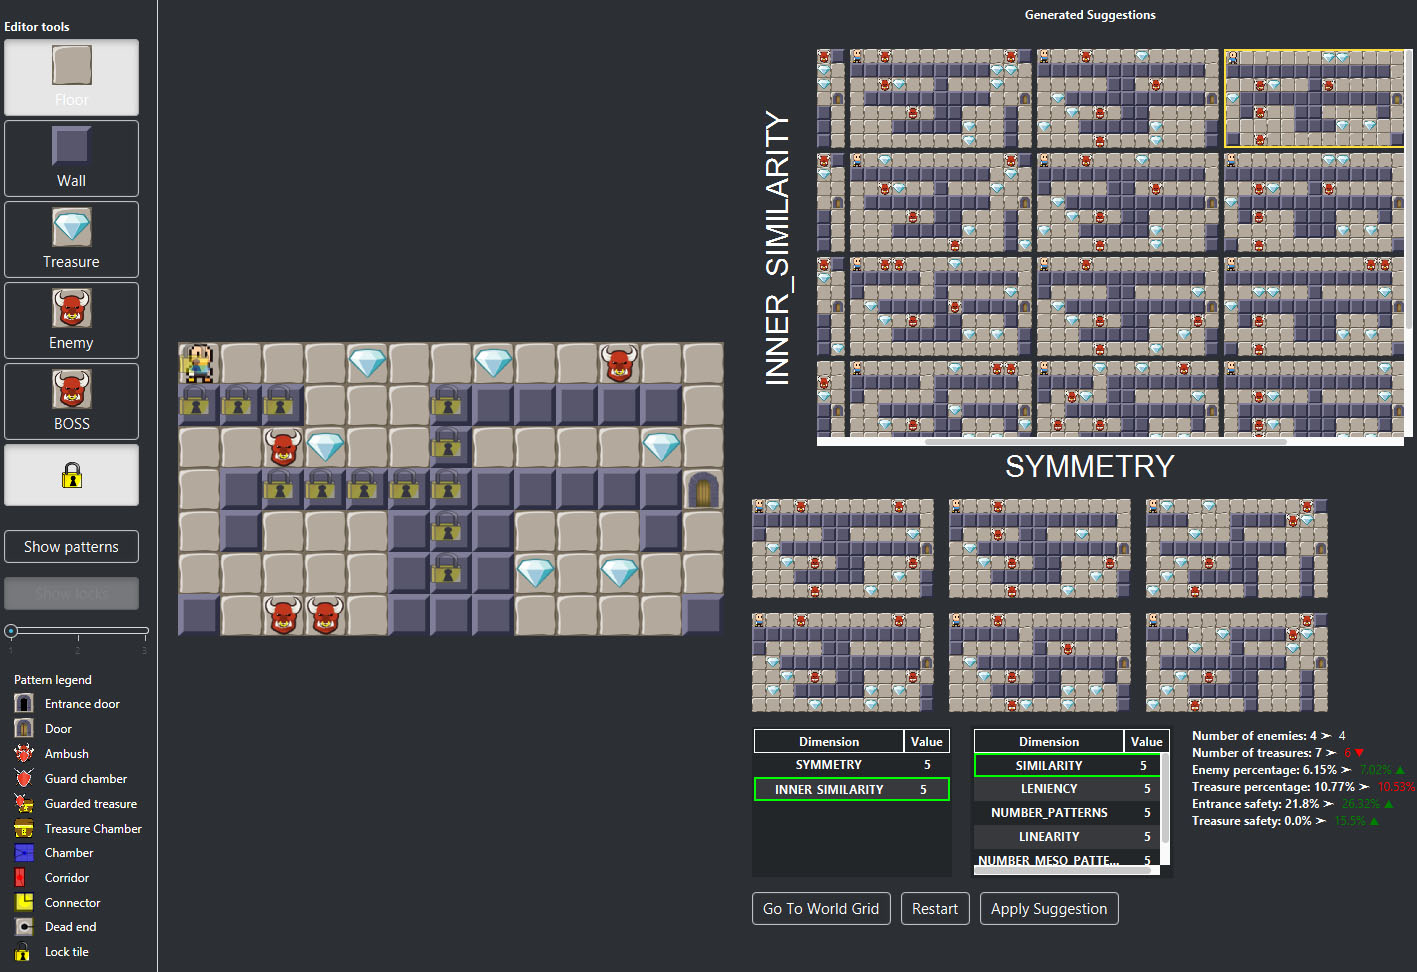
\includegraphics[width=9cm]{figures/figure1.png}}
% \caption{The main components in EDD. (a) A basic room, (b) different placeable tiles, (c) micro-patterns and (d) meso-patterns~\cite{p6Alvarez2018a}.}
% \label{figs:basecomponents}
% \end{figure}
\subsection{Background}

% Machine Learning (ML) has gained an increased interest from game researchers, achieving remarkable success on training AI agents for very popular games, such as AlphaStar on Starcraft 2 \citepsixth{p6alphastarblog} and OpenAI Five on Dota 2 \citepsixth{p6berner2019dota}. Its combination with PCG has led to the raise of  Procedural Content Generation via Machine Learning (PCGML), defined as the generation of game content by models that have been trained on existing game content \citepsixth{p6summerville2018procedural}, with applications to autonomous content generation, content repair, content critique, data compression, and mixed-initiative design. 

Player modeling, the ability to recognize general socio-emotional
and cognitive/behavioral patterns in players \citepsixth{p6thawonmas2019artificial}, has been appointed by the game research community as an essential process in many aspects of game development, such as designing of new game features, driving marketing and profitability analyses, or as a means to improve PCG and game content adaptation. Player modeling frequently relies on data-driven and ML approaches to create such models out of several sorts of user-generated gameplay data \citepsixth{p6liapismodellingquality19,p6melhart2020feel,p6Drachen2009-playerModellingTombRaider,p6Holmgard2019-proceduralPersonas,p6Melhart2019-ModellingMotivation}.

Using player data from \textit{Iconoscope}, a freeform creation game for visually depicting semantic concepts, Liapis et al. trained and compared several ML algorithms by their ability to predict the appeal of an icon from its visual appearance~\citepsixth{p6liapismodellingquality19}. Furthermore, Alvarez and Vozaru explored personality-driven agents based on individuals' personalities using the \textit{cibernetic big five model}, evaluating how observers judged and perceived agents using data from their personality test when encountering multiple situations~\citepsixth{p6Alvoz2019-PersonalityDriven}. 

%  using Bartle's player archetypes~\citepsixth{p6bartle1996-taxonomy}

Moreover, training models on gameplay data from \textit{Tom Clancy's The Division} has also been used to model, and therefore find predictors of player motivation \citepsixth{p6Melhart2019-ModellingMotivation}, which renders a very valuable tool for understanding the psychological effects of gameplay. Former research followed a similar approach in \textit{Tomb Raider Underworld}, training player models on high-level playing behavior data, identifying four types of players as behavior clusters, which provide relevant information for game testing and mechanic design \citepsixth{p6Drachen2009-playerModellingTombRaider}. Melhart et al. take these approaches one step further by modeling a user's \textit{Theory of Mind} in a human-game agent scenario \citepsixth{p6melhart2020feel}, finding that players' perception of an agent's frustration is more a cognitive process than an affective response. %Alvarez and Vozaru did similar work, exploring personality-driven agents based on individuals' personality using the \textit{cibernetic big five model}, evaluating how observers judged and perceived agents using data from their personality test when encountering multiple situations~\citepsixth{p6Alvoz2019-PersonalityDriven}.

%Alvarez and Vozaru did similar work, exploring personality-driven agents based on individuals' personality using the \textit{cibernetic big five model}, which treats personality-driven agents as goal-based entitites, evaluating how observers judged and perceived agents using data from their personality test when encountering multiple situations~\citepsixth{p6Alvoz2019-PersonalityDriven}.
%modeling individual agents based 

\subsubsection{The Player is the Designer}

Mixed-initiative co-creativity (MI-CC)~\citepsixth{p6yannakakis2014micc}, is the subset of PCG algorithms where human users and AI systems engage in a constant mutual inspiration loop towards the creation of game content \citepsixth{p6charity2020baba,p6machado2019pitako,p6shaker2013ropossum,p6smith_tanagra:_2011,p6liapis_generating_2013}. Understanding player behavior and experience, as well as predicting the player's motivation and intention is key for mixed-initiative creative tools while aiming to offer in real-time user-tailored procedurally generated content. Nevertheless, the player is the designer in MI-CC, and gameplay data is replaced by a compilation of designer-user actions and AI model reactions over time while both user and model are engaged in a mutually inspired creative process. A fluent MI-CC loop should provide good human understanding and interpretation of the system, as well as accurate user behavior modelling by the system, capable of projecting the user's subsequent design decisions \citepsixth{p6ComptonPhD}. 

%Similar to user or player modeling, designer modeling for content creation tools (CAD and MI-CC tools) was suggested by Liapis et al~\citepsixth{p6Liapis2013-designerModel}, where it is proposed the use of designers models that capture their styles, preferences, goals, intentions, and interaction processes. In their work, they suggest methods, indications, and advice on how each part can be model to be integrated into a holistic designer model, and how each game facet can use and benefit from designer modeling. Moreover, in \citepsixth{p6Liapis2014-designerModelImpl} the same authors discuss their implementation of designer modeling and the challenges of integrating all together in their MI-CC tool, Sentient Sketchbook, which had a positive outcome on the adaptation of the tool towards individual “artificial” users.

Shifting towards a designer-centric perspective means that besides focusing on player modeling, it is necessary to focus on modeling the designers. Liapis et al.~\citepsixth{p6Liapis2013-designerModel,p6Liapis2014-designerModelImpl} introduced designer modeling for personalized experiences when using computer-aided design tools, with a focus on the integration of such in automatized and mixed-initiative content creation. The focus is on capturing the designer's style, preferences, goals, intentions, and iterative design process to create representative models of designers. Through these models, designer's and their design process could be understood in-depth, enabling adaptive experiences, further reducing their workload and fostering their creativity. 

%\citepsixth{p6charity2020baba,machado2019pitako,shaker2013ropossum,smith_tanagra:_2011,Machado2017,liapis_generating_2013}. 

% Moreover, goal 13 in the guidelines for Human-AI interaction \citepsixth{p6amershi2019guidelines} highlights the importance of learning from user behavior and personalize the user’s experience by learning from their actions over time. 


%Nourani et al.~\citepsixth{p6Nourani2019-meaningfulExplanations}, who discuss the effects of meaningful and meaningless explanations to users of an AI interactive systems, and their results demonstrates that when an explanation is not aligned with human-logic it significantly affect the user's perception of the system and it's usability is hindered.

Furthermore, lack of transparency is a key impediment for the advancement of human-AI systems, being eXplainable AI (XAI) an emergent research field that holds substantial promise for improving model explainability while maintaining high-performance levels~\citepsixth{p6adadi2018peeking,Doshi-Velez2018}. However, explanations should be aligned with the users' understanding to don't hinder the usability of systems, as demonstrated by Nourani et al.~\citepsixth{p6Nourani2019-meaningfulExplanations}, who discuss the effects of meaningful and meaningless explanations to users of an AI interactive systems.

Zhu et al.~\citepsixth{p6Zhu2018-XAIDesignersMICC} proposed the field of eXplainable AI for Designers (XAID) as a human-centered perspective on MI-CC tools. This work discusses three principles of mixed-initiative, \emph{explainability}, \emph{initiative}, and \emph{domain overlap}, where the latter focuses on the study of the overlapping creative tasks between game designers and black-box PCG systems in mixed-initiative contexts. This work deems of high relevance the inclusion of data-driven and trained artifacts to facilitate a fluent bi-directional communication of the internal mechanisms of such a complex co-creative process in which \textit{the designer provides the vision, the AI provides capabilities, and they merge that into the creation}. Mapping the designer's internal model to the AI's internal model is suggested as a meaningful way for creating a common ground that establishes a shared language that enables such communication. In the same line, Xie et al.~\citepsixth{p6xie2019interactive} explored visualization techniques through an interactive level designer tool called \textit{QUBE} to explain and introduce machine learning principles to game designers.

Moreover, Guzdial et al.~\citepsixth{p6guzdial-lvldsg-aiide-2018} discuss the insufficiency of current approaches to PCGML for MI-CC, as well as the need for training on specific datasets of co-creative level design. Guzdial et al. work on the mixed-initiative Morai Maker~\citepsixth{p6guzdial2019friend} shows the relevance of exploring the ways designers and AI interact towards co-creation, identifying four human-AI relationships (friend, collaborator, student, and manager), as well as the different ways they impact on the designer-user experience. Our study advocates for the importance of designer modeling through ML as the generation of surrogate models of designer styles by training on existing designer-generated data, aiming for an improvement in quality and diversity in computational creativity and, in particular, MI-CC tools. 

\subsubsection{The Designer Preference Model in EDD}

EDD is an MI-CC tool where designers can create dungeons and rooms; meanwhile, a PCG system analyzes their design and proposes generated suggestions to the designer~\citepsixth{p6Alvarez2018, Baldwin2017}. EDD uses the \emph{Interactive Constrained MAP-Elites} (IC-MAP-Elites)~\citepsixth{p6alvarez2019empowering}, an evolutionary algorithm that combines Constrained MAP-Elites~\citepsixth{p6Khalifa2018} with interactive and continuous evolution. 

The work presented in \citepsixth{p6Alvarez2020-DesignerPreference} introduced the Designer Preference Model, a data-driven solution that learns from user-generated data in the MI-CC Evolutionary Dungeon Designer. This preference model uses an Artificial Neural Network to model the designer based on the choices she makes while using EDD. Both systems constantly interact and depend on each other, so that the Designer Preference Model learns from the generated and selected elites, and IC-MAP-Elites uses the Designer Preference Model as a surrogate model of the designer to complement the fitness evaluation of new individuals. 

This approach's main goal is modeling the user's design style to better assess the tool's procedurally generated content, increasing the user's agency over the generated content without stalling the MI-CC loop \citepsixth{p6ComptonPhD} or increasing user fatigue with periodical suggestion handpicking \citepsixth{p6liapis2016mixed,p6Takagi2001-InteractiveEvo}. The results showed the need for stability and robustness in the data-driven model, to counterbalance the highly dynamic designer's creative process. 


\subsection{Room Style Clustering}

% \begin{enumerate}
%     \item Information on the user studies and how we develop the clusters.
%     \item collected data through 2 user studies
%     \item transformed the data into 5 datasets
%     \item data reduction through PCA and T-SNE. Cluster with K-means, K-Medoids, agglomerative clustering and DBSCAN. Evalulated through internal indices (silhouette index, DB index, and CH-index) 
% \end{enumerate}

\begin{figure*}[ht!]
\centerline{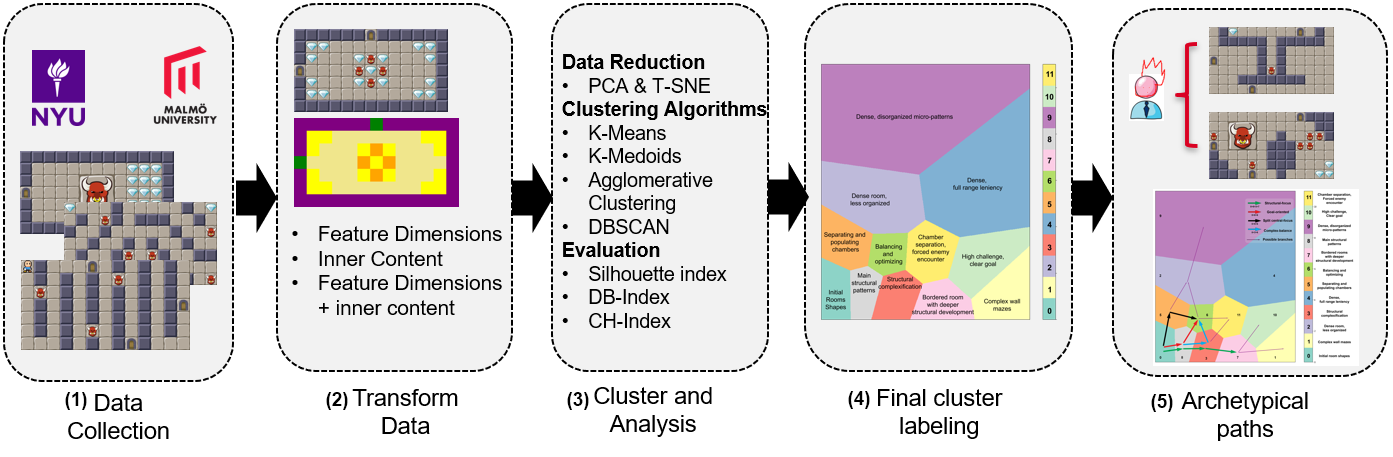
\includegraphics[width=\textwidth]{figures/process-steps.png}}
\caption{The stages of the design style clustering development: (1) Data was first collected through two user studies. (2) Then, using the design sequences, the data was processed into five different datasets, one using the room images, a second using the tiles information, and three using tabular information. (3) A data reduction technique was applied to different datasets, and then they were clustered and internally evaluated. (4) The clusters were formed, picked from the best performing methods, and labeled based on the data points within each cluster. The cluster were evaluated by visualizing how a typical design session traverse the various clusters, and K-Means (K=12) was chosen as the final approach. (5) Finally, using this final approach all the sequences were clustered and archetypical paths were identified.%(5) The final approach,  K-Means (K=12) was evaluated by visualizing how a typical design session traverse the various clusters. Finally, the sequences were clustered by the final approach and archetypical paths were identified.
} \label{p6fig:approach-steps}
\end{figure*}

\begin{figure*}[t]
\centerline{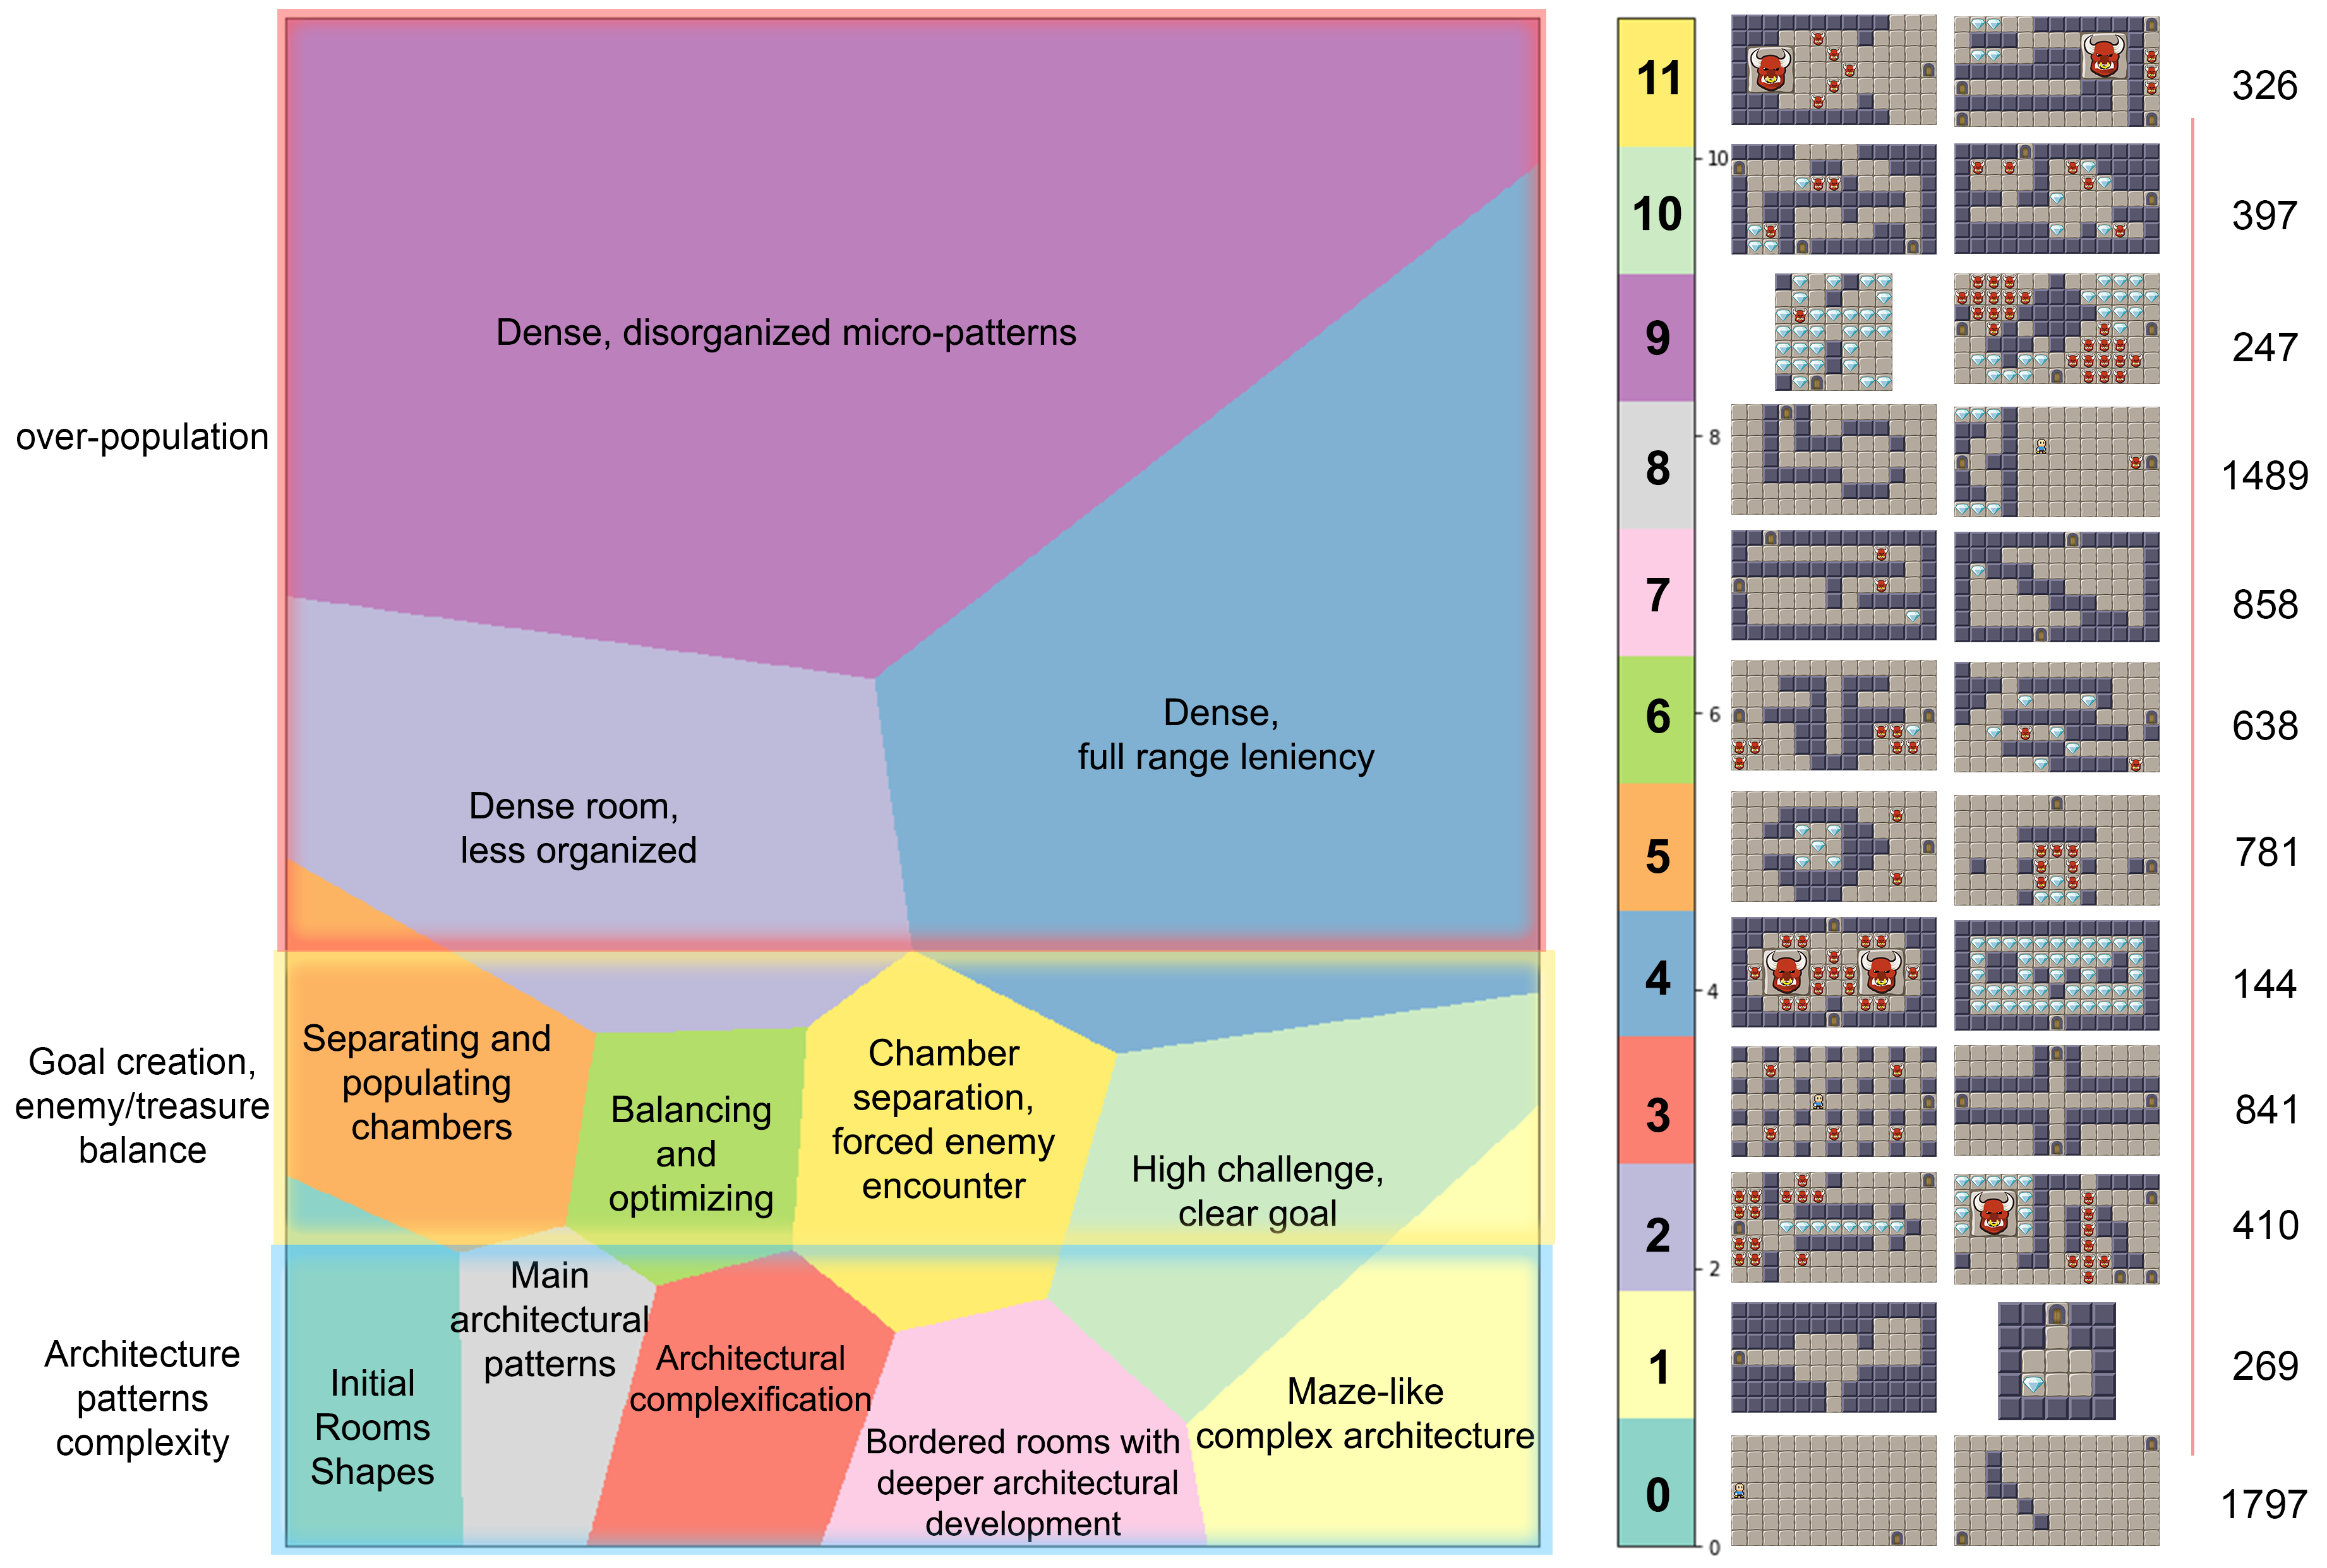
\includegraphics[width=\textwidth]{figures/final-cluster.png}}
\caption{Best resulting cluster set. K-Means (K=12), using the \textbf{Tiles} Dataset. While it scores slightly less in the internal indices that other setups, a qualitative analysis successfully gives us more granularity by subdividing the main bottom clusters, to label and cluster the design process of designers. Sample rooms belonging to each cluster are displayed on the right, next to the total number of rooms in the cluster.} \label{p6fig:all-clusters}
\end{figure*}

% \begin{figure*}[b]
% \centerline{\includegraphics[width=13cm]{figures/representative cluster-steps.png}}
% \caption{Examples of a step by step edition sequence of a design session and it's clustering. To the left, we present the actual sequence and steps of one of the rooms in the dataset and to the right is the actual trajectory of the design in the cluster space. Numbered and in black, it is shown how each step of the design process is clustered by our approach} \label{p6fig:paths-designers}
% \end{figure*}

% \begin{figure}[h]
% \centerline{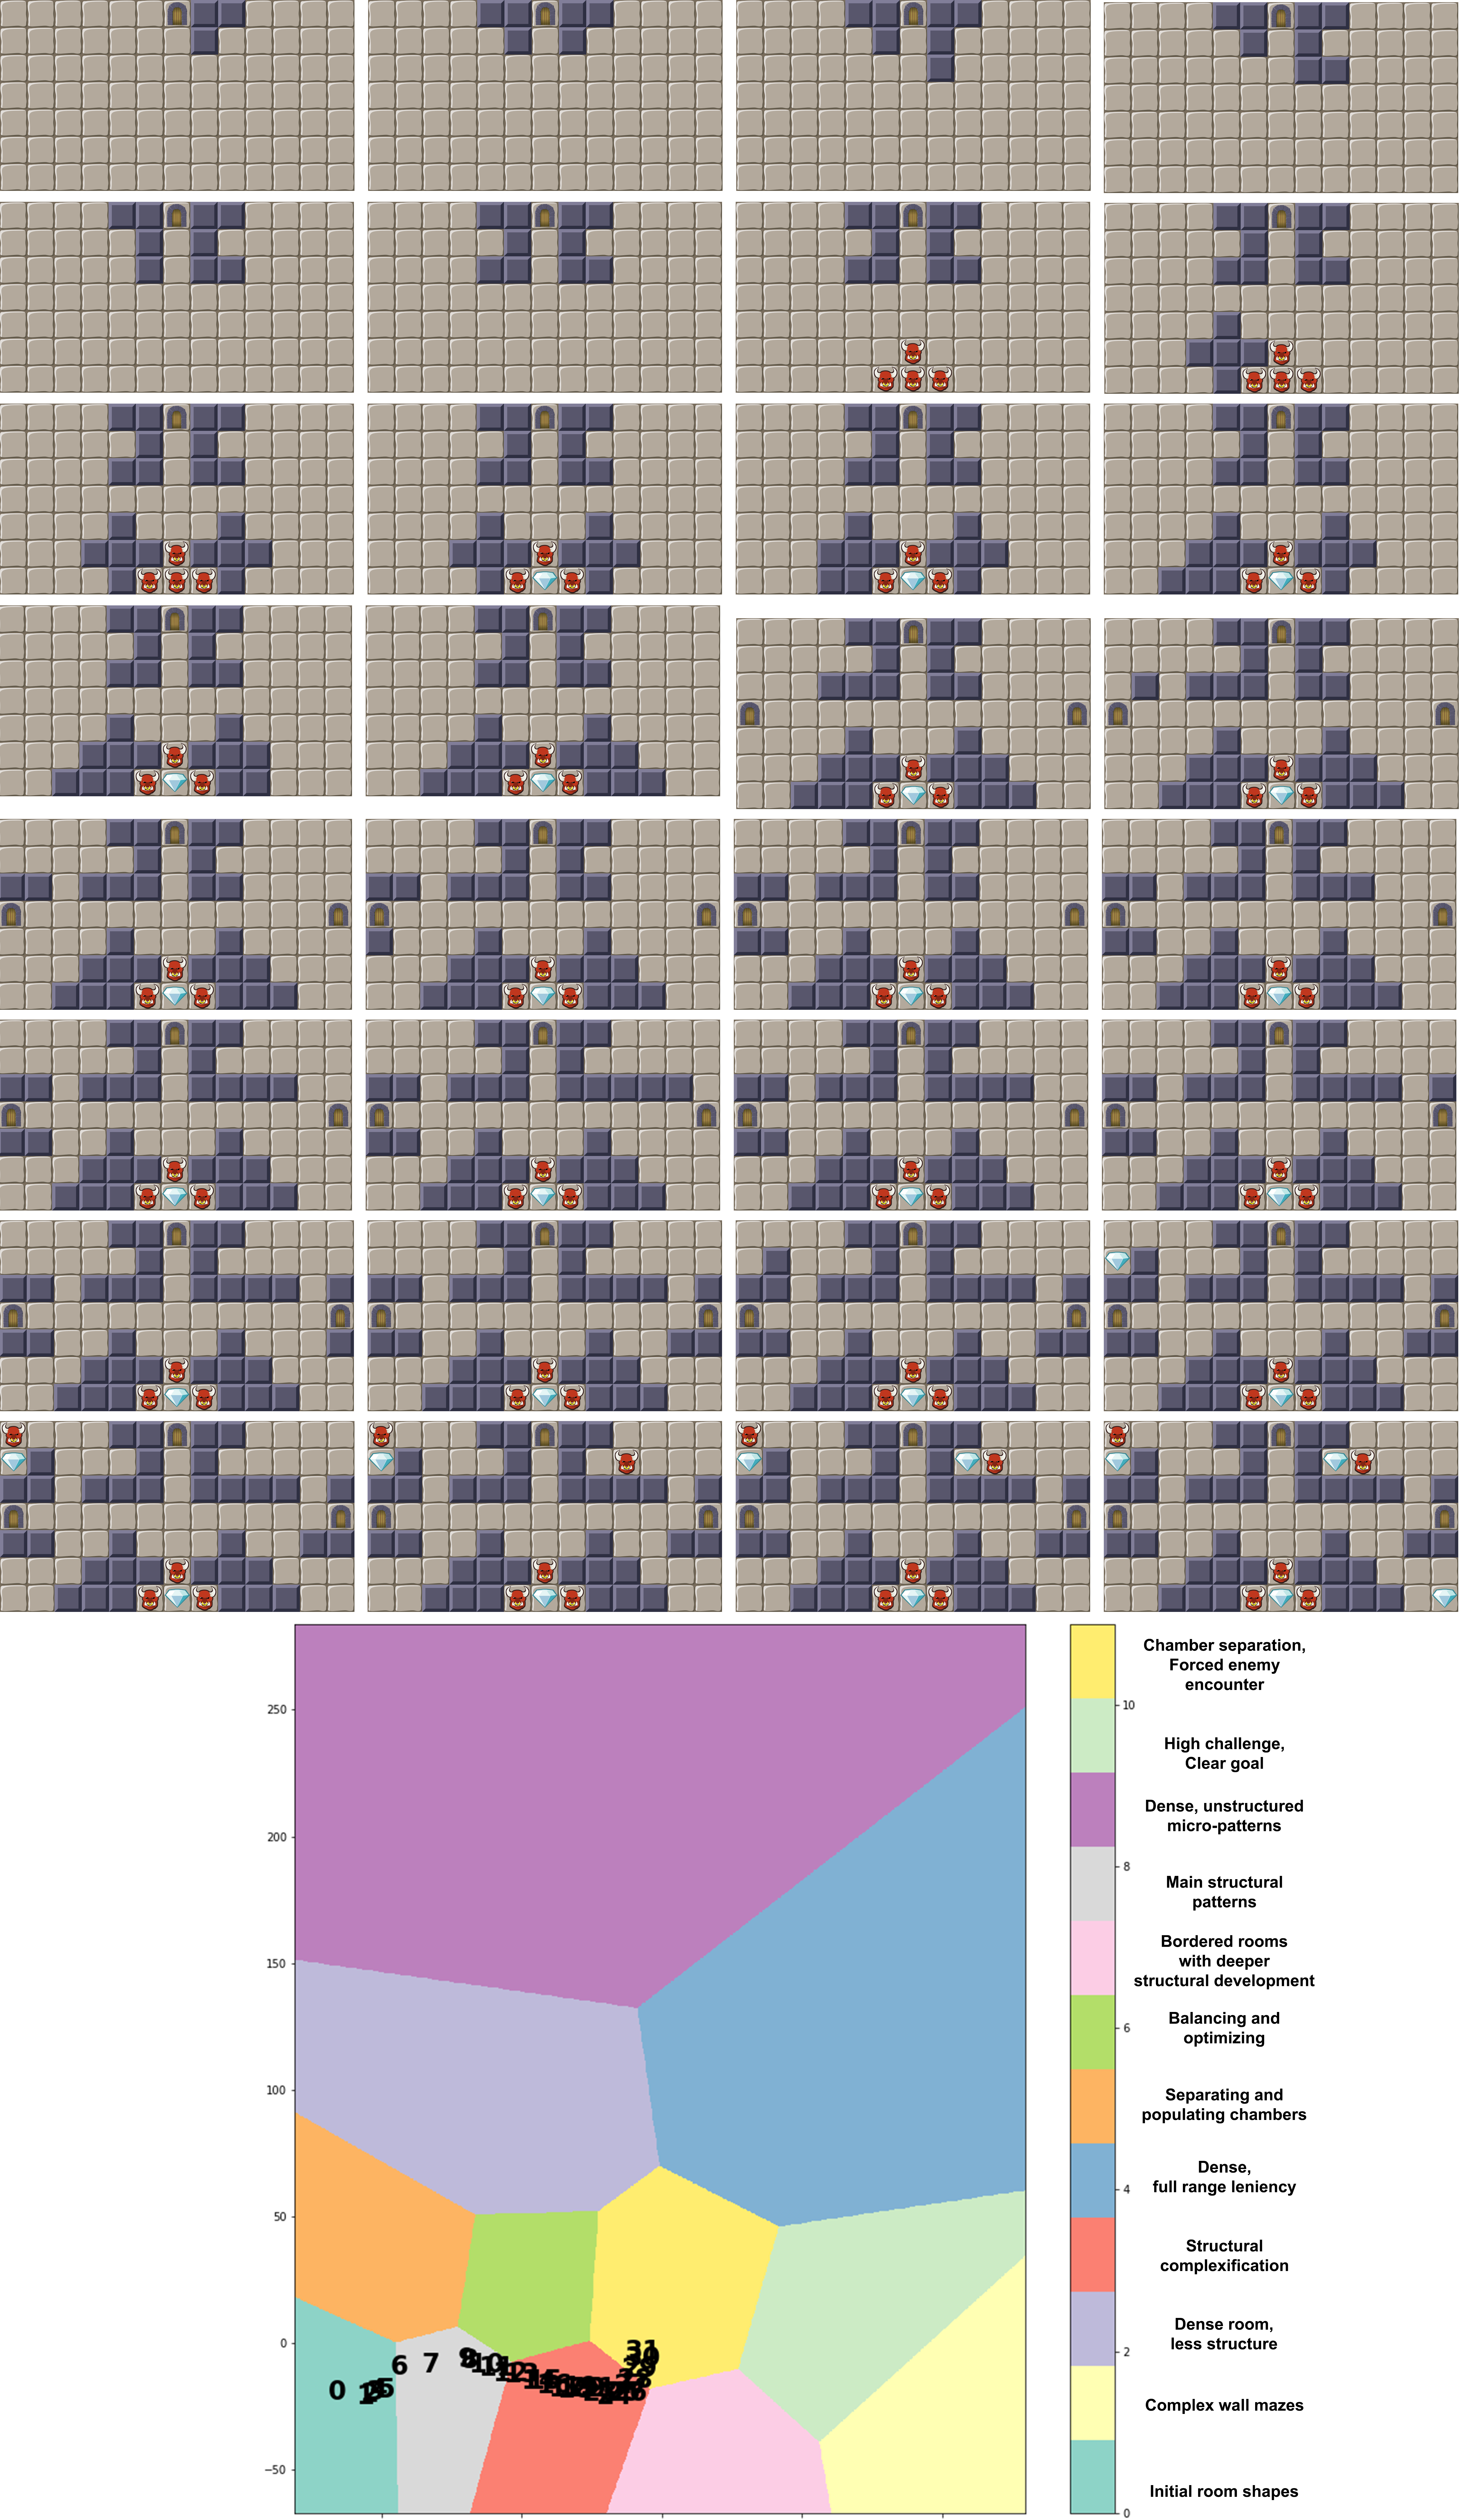
\includegraphics[width=8cm]{figures/representative-cluster-steps-alter.png}}
% \caption{Example of a step by step edition sequence of a design session and it's clustering. At the top, we present the actual sequence and steps of one of the rooms in the dataset, in a $4\times7$ grid, starting at the top left with the first edition. At the bottom, it is the actual trajectory of the design in the cluster space. Numbered and in black, it is shown how each step of the design process is clustered by our approach} \label{p6fig:paths-designers}
% \end{figure}

\begin{figure*}
\centerline{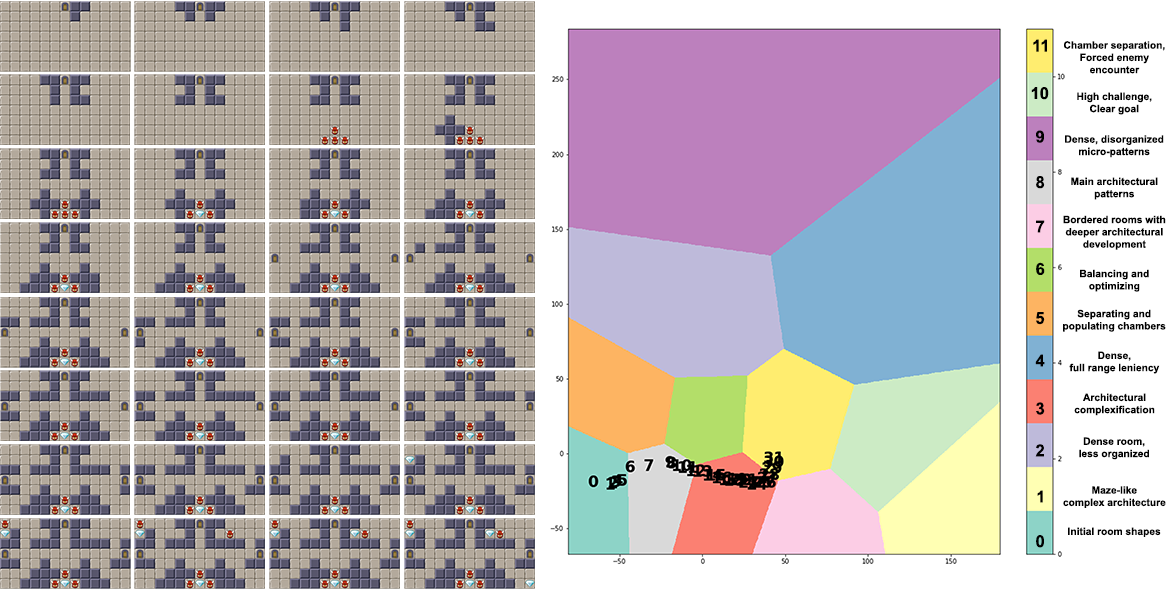
\includegraphics[width=\textwidth]{figures/representative-clusters-small.png}}
\caption{Example of a step by step edition sequence of a design session and it's clustering. At the left, we present the actual sequence and steps of one of the rooms in the dataset, in a $4\times7$ grid, starting at the top left with the first edition. At the bottom, it is the actual trajectory of the design in the cluster space. Numbered and in black, it is shown how each step of the design process is clustered by our approach} \label{p6fig:paths-designers}
\end{figure*}

This paper presents an approach and fundamental steps towards the implementation of designer personas: an analysis of designer style clustering to isolate archetypical paths that can be later be used to build ML surrogate models of archetypal designers. Such models would adapt to the dynamic designer during the mixed-initiative creative process by being placed in the solution space, allowing the designer to traverse such space of models as she drifts through the many dimensions of her creative process.

The proposed system builds on top of EDD's Designer Preference Model and preliminary results \citepsixth{p6Alvarez2020-DesignerPreference}, expanding it to classify the designers' designs based on clusters developed using previously hand-made design sequences by expert and non-expert designers. Figure \ref{p6fig:approach-steps} illustrates our approach in five sequential stages, from data collection to experimentation and results. The first four stages are explained in the following subsections, whereas Section~\ref{p6section:results} shows the experimental results.

\subsubsection{Data Collection}

We conducted two user studies where participants were tasked with freely designing a dungeon in EDD and the rooms that compose it with no further restrictions, using all the available tiles i.e. floor, wall, treasure, enemy, and boss tiles. All participants were introduced to the tool before the design exercise. User-generated data was gathered during the complete design session, creating a new data entry every time the designer edited the dungeon. In total, we had $40$ participants, $25$ of these (i.e. NYU participants) were industry or academic researchers within the Games and AI field, and the other $15$ (i.e. MAU participants) were game design students. This resulted in a diverse dataset composed of $180$ unique rooms like the ones depicted in Figure~\ref{p6fig:approach-steps}, that was pre-processed and clustered in the subsequent stages. 

\subsubsection{Dataset pre-processing}

From the $180$ unique rooms, we extracted and used the edition sequence of each of the rooms, from their initial design to the more elaborated end-design, to compose a richer dataset that could capture the design process of a designer rather than focusing on the end-point. Through this, we ended up using $8196$ data points in our dataset.
%just the end-point. We ended up using $8196$ rooms
Moreover, five different copies of the dataset were created to analyze and compare the performance of the clustering stage using the following image pre-processing methods:

\begin{enumerate}
\setcounter{enumi}{0}
    \item \textbf{Room:} No pre-processing. Room images are fed into the next stage as they were created by the designer, with a resolution of $1300\times 700\times3$, corresponding to width, height, and RGB ($3$ color channels).
    
    \item \textbf{Tiles:} Each room tile type is mapped to a single-color pixel and the rooms are simplified to a pixel-tile based representation, as shown in the second stage of Figure \ref{p6fig:approach-steps}. The dimensions are downscaled to $13\times 7\times3$.
    %Each room tile is simplified to a single-color pixel, as shown in the second stage of Figure \ref{p6fig:approach-steps}, downscaled to $13\times 7\times3$.
    
    \item \textbf{Dimensions:} Each room is described by its five IC-MAP-Elites feature dimension values, excluding the similarity scores: \textsc{Linearity}, \textsc{Leniency}, \textsc{\#MesoPatterns}, \textsc{\#SpatialPatterns}, and \textsc{Symmetry}. A complete description of these features can be found in~\citepsixth{p6Alvarez2020-ICMAPE}.
    
    \item \textbf{Inner Content:} Each room is described by $12$ values, related to the count, sparsity, and density of the enemy, treasure, floor, and wall tiles contained in it.
    
    \item \textbf{Combined:} A combination of the \textbf{Dimensions} and \textbf{Inner Content} methods.
\end{enumerate}

\subsubsection{Clustering and Analysis}

To run all setups, data reduction algorithms, clustering algorithms, and do the internal evaluation of the clusters, we used scikit-learn machine learning toolset~\citepsixth{p6scikit-learn}. To obtain the best set of clusters, we ran different setups with the above datasets. The data was reduced to two meaningful dimensions with two different data reduction algorithms, Principal Component Analysis (PCA) and T-Distributed Stochastic Neighbor Embedding (T-SNE). For both data reduction algorithms, we fit the algorithms with each individual dataset, setting to two principal components and in the case of T-SNE using PCA as initializing algorithm, and transforming the data into a new dataset \emph{pca\_dataset} and \emph{tsne\_dataset} per dataset. Each two-dimensional point in the new datasets represents a step in the sequences described above.%Likewise, for the T-SNE, we fit the algorithm with each individual dataset, setting the parameters to two principal components and using PCA as initializing algorithm, and then transformed the data into a new dataset \textit{tsne_dataset} per dataset.

Moreover, all the resulting datasets were then clustered using \textsc{K-Means, K-Medoids, Agglomerative clustering}, and \textsc{DBSCAN}. K-Means was initialized using the standard k-means++ implemented in scikit-learn, which initialize all centroids distant from each other. K-Medoids was initialized similarly, using the standard k-medoids++, and tested using the \emph{cosine}, \emph{euclidean}, and \emph{manhattan} distances. Agglomerative clustering is a hierarchical clustering approach using a bottom-up approach implemented in scikit-learn using four different linkage criteria for comparing data points: \emph{Ward}, \emph{Complete}, \emph{Average}, and \emph{Single}. Finally, DBSCAN cluster points based on density separated by low-density areas; thus, DBSCAN automatically finds $k$ based on two parameters, $\epsilon$ describing the maximum distance between points and \emph{min\_samples} describing the minimum amount of samples within a group to be considered a cluster. K-Means, K-Medoids, and Agglomerative clustering were tested using multiple $K$ values ranging from 3 to 13, and DBSCAN was tested with several $\epsilon$ values ranging from 0.3 to 1.0, and \emph{min\_samples} ranging from 2 to 9.

%, testing with $K$ values ranging from 3 to 13 for the first three ones, and several $\epsilon$ values for DBSCAN.

%testing different minimum distance between data points ($\epsilon$) and the minimum amount of data points within a cluster to be considered a dense region for DBSCAN.

Since we lack a labeled dataset (i.e. ground truth) for cluster validation, we evaluated the results from all setups using the internal indices below, as well as manually inspecting the rooms composing the resulting clusters.

%Since in our approach lacks a labeled dataset (i.e. ground truth) for cluster validation, 

\begin{itemize}
\item \textbf{Silhouette Score:} The Silhouette Score shows how similar a data point is to the cluster it is associated with, through calculating the difference between the $\overline{distance}$ from the point to the points in the nearest cluster and the $\overline{distance}$ to the points in the actual cluster. The value is bounded from -1 to +1, with values closer to +1 indicating a good separation of the clusters, and closer to -1 meaning that some points might belong to another cluster.
\item \textbf{Davies-Bouldin Index:} The DB-index is the ratio between the within-cluster distances and between-clusters distances. With this, we can have an insight into the average similarity of clusters with their closest cluster. The value is bounded from 0 to +1, with values closer to 0 relate to clusters that are farther apart from each other and less dispersed, thus, this index is more crucial when we have more dense representations.
\item \textbf{Calinski-Harabasz Index:} The CH-index is another index related to the density of the clusters and how well separated they are. The score is the ratio between the within-cluster dispersion (compactness) and the between-cluster dispersion (separation). The CH-index is positively unbounded, and the higher the score the better.
\end{itemize}

\subsubsection{Cluster Labelling}

\begin{table}
\begin{center}
{\caption{Best performing setups based on their internal validation and visualization of clustered data points.}\label{p6table:setups}}
\resizebox{0.9\textwidth}{!}{
\begin{tabular}{ccccccc}
\hline
\rule{0pt}{12pt}
Algorithm&Data&K&$\Diamond$&$\Box$&$\bigtriangleup$ 
\\ 
\hline
\\[-6pt]
K-Means & Tiles-PCA & 9 & 0.43 & 0.73 & 9438.233 \\ 
K-Means & Tiles-PCA & 12 & 0.41 & 0.77 & 9436.928 \\
K-Means & Dimensions-PCA & 12 & 0.43 & 0.73 & 7738.343 \\
Agglomerative single & Combined-PCA & 6 & 0.51 & 0.43  & 38.833 \\ 
Agglomerative avg. & Dimensions-PCA & 6 & 0.44 & 0.67 & 3463.567 \\ 
\hline
\\[-6pt]
\multicolumn{6}{l}{$\Diamond$ Silhouette Score\ \
$\Box$ Davies Bouldin Index\ \
$\bigtriangleup$ Calinski-Harabasz Index}
\end{tabular}
}\end{center}
\end{table}

Table~\ref{p6table:setups} shows the best performing setups according to their internal indices scores. The clusters in these setups were manually inspected in order to detect the qualitative features that better define them. 

When using the \textbf{Dimensions} and \textbf{Combined} datasets, the clusters do perform good, if not better, in certain indices than when using the \textbf{Tiles} dataset. However, when analysing the resulting setups, they were missing a clearer relation between the clustered rooms, which was exacerbated when analysing sequences and paths on these setups, where they missed continuity between clusters.

Conversely, given that we are creating tile-based rooms and dungeons, the features were more representative for the \textbf{Tiles} dataset, which when used, generally performed well in the evaluated internal indices, and the produced clusters meaningfully separate the data. Further, as it will be presented in Section \ref{p6section:results}, when clustering sequences and analyzing the cluster path of the designs, there exist a continuity between designs that supports its usability. Figure \ref{p6fig:all-clusters} shows the best-resulting cluster set found among all the experiments run.



% As expected, the \textbf{Tiles} dataset generally performed well in the evaluated internal indices, and the produced clusters meaningfully separated the data.
% better information and were meaningfully group together.  relation each of the features have with 

% As expected, the \textbf{Tiles} representation have good results across the 3 indices, 

% JOSÉ: I leave it here waiting for the final results from Alberto

%Moreover, We noticed that the agglomerative approach results in very specific clusters alongside a quite broad cluster consisting of unrelated data points, regardless of the $K$ used. These setups scored well in the different indices but fail to accurately partition the space in relevant groups.

%Moreover, there are recurrent clusters between the different setups but when using more clusters like in figure~\ref{p6fig:all-clusters} (b), we can have more granularity when partitioning the space, improving the separation of more related data points. In figure~\ref{p6fig:all-clusters}(b) we present several rooms that have been clustered together matching the labeling of the clusters. In the figure, there is a clear correlation between the designs and the labels of their respective cluster, and an interesting continuity between the final clusters.

% In Figure~\ref{p6fig:all-clusters}, we present the final and selected approach for clustering room styles using K-Means (K=12) and the \textbf{Tiles} dataset reduced with the PCA algorithm. To the right, next to each color in the legend, we have different representative rooms that belong to the clusters, in their respective color, and have been clustered together. Furthermore, besides the local relation between clusters, there exists a layered division among group of clusters in the y-axis, where the bottom clusters relate more to architectural pattern complexity, from very empty rooms to mazes. The middle clusters focus on populating the rooms with enemies and treasures, creating the actual goals of the room and balancing the challenge. Finally, the top clusters are composed of dense rooms where the enemy and treasure addition do not necessarily need to follow any clear objective. 


% The clusters's label are plotted on top of each of the clusters, describing in general, the content that is within them. These cluster 

In the figure, we have plotted on top of the clusters the labels describing in general, the content that is within them. The following is a description of the clusters and the rooms that were clustered together:

\textbf{0. Empty-Initial rooms:} %This cluster contains $1797$ data points, and 
This cluster relates mostly to the initial designs made by the designers. These designs are from completely empty rooms to initial work-in-progress structures.

\textbf{1. Maze-like complex architecture:} This cluster to the extreme of the architectural patterns complexity layer, relates to more highly-linear, confined and maze-like rooms.% with more structure on what is possible. %The cluster contains $269$ data points.

\textbf{2. Dense, less organized:} This cluster contains rooms that still have a certain objective but are moving towards more disorganized distributions of micro-patterns in relation to their density. %This cluster contains $410$ data points.

\textbf{3. architectural complexification:} %This cluster contains $841$ data points, and 
This cluster relates mostly to the complexification of wall structures by having dense wall chunks, representative architectural patterns, or symmetrical patterns.

\textbf{4. Dense, full range leniency:} Focusing on density as the other two clusters within the same layer, this cluster relates to rooms that are in the full range of leniency from very rewarding, treasure rooms to very challenging boss rooms. %This cluster contains $144$ data points.

\textbf{5. Separating and populating chambers:} This cluster relates to the process of separating rooms into distinct chambers, focusing on the center of the room, and starting to populate rooms with enemies and treasures. %The cluster contains $781$ data points.

\textbf{6. Balancing and optimizing:} This cluster contains a mix between corridors and chambers within rooms with a focus on balancing rooms and optimizing their design towards certain goals. %The cluster contains $638$ data points.

\textbf{7. Bordered rooms with deeper architectural development:} This cluster relates mostly to rooms with an added wall border by the designer, and where the focus is to shape chambers and develop more visual structures.

\textbf{8. Main architectural shapes:} Similar to other clusters within the same layer, this cluster relates to the development and definition of main architectural patterns that are somewhat symmetric.

\textbf{9. Dense, disorganized micro-patterns:} This cluster clusters the extreme rooms that contain a high density of tiles, other than floor-tiles, without a clear structure or objective for the player.

\textbf{10. High challenge, clear goal:} This cluster relates to well-shaped rooms with clear wall structures and goals, towards more challenge. 

\textbf{11. Chamber separation with forced enemy encounter:} This cluster relates to rooms that are in the process of a clear segmentation into corridors and chambers, and that enforce to some extent, enemy encounters for the player. 

Furthermore, besides the local relation between clusters, the clusters are implicitly divided in three layers on the Y-axis. From bottom to top, (a) architectural patterns complexity, relating to clusters composed of rooms with clearer or complex shapes done with walls, from empty rooms to mazes. (b) Goal creation, enemy/treasure balance, with clusters comprehending the strategic addition of enemies and treasures to establish objectives in the room for the player. In terms of EDD, these rooms are composed of more meso patterns. And (c), over-population, which relates to clusters filled with less organized and dense rooms where the enemy and treasure addition do not necessarily need to follow any clear objective. Identifying the designer in such layer, and the path they have taken to get there could show meaningful information in the design process. For instance, the intentions of the designer, in what phase of the design process she is at the moment i.e. trying the tool or observing how the tool reacts or scraping her current goal towards a new goal within the room. 

% \begin{enumerate}
% \setcounter{enumi}{-1}
% \item[0] \textbf{Empty/Initial rooms:}
% \item \textbf{Complex wall mazes:} 
% \item \textbf{Dense, less structure} 
% \item \textbf{Structural complexification:} 
% \item \textbf{Dense, full range leniency} 
% \item \textbf{Separating and populating chambers:} 
% \item \textbf{Balancing and optimizing rooms:} 
% \item \textbf{Bordered rooms with deeper structural development:}
% \item \textbf{Development of main structural shapes:} 
% \item \textbf{Dense, unstructured:} 
% \item \textbf{Challenging rooms with clear goal:} 
% \item \textbf{Chamber separation with forced enemy encounter:} 
% \end{enumerate}



\begin{figure*}[t!]
\centerline{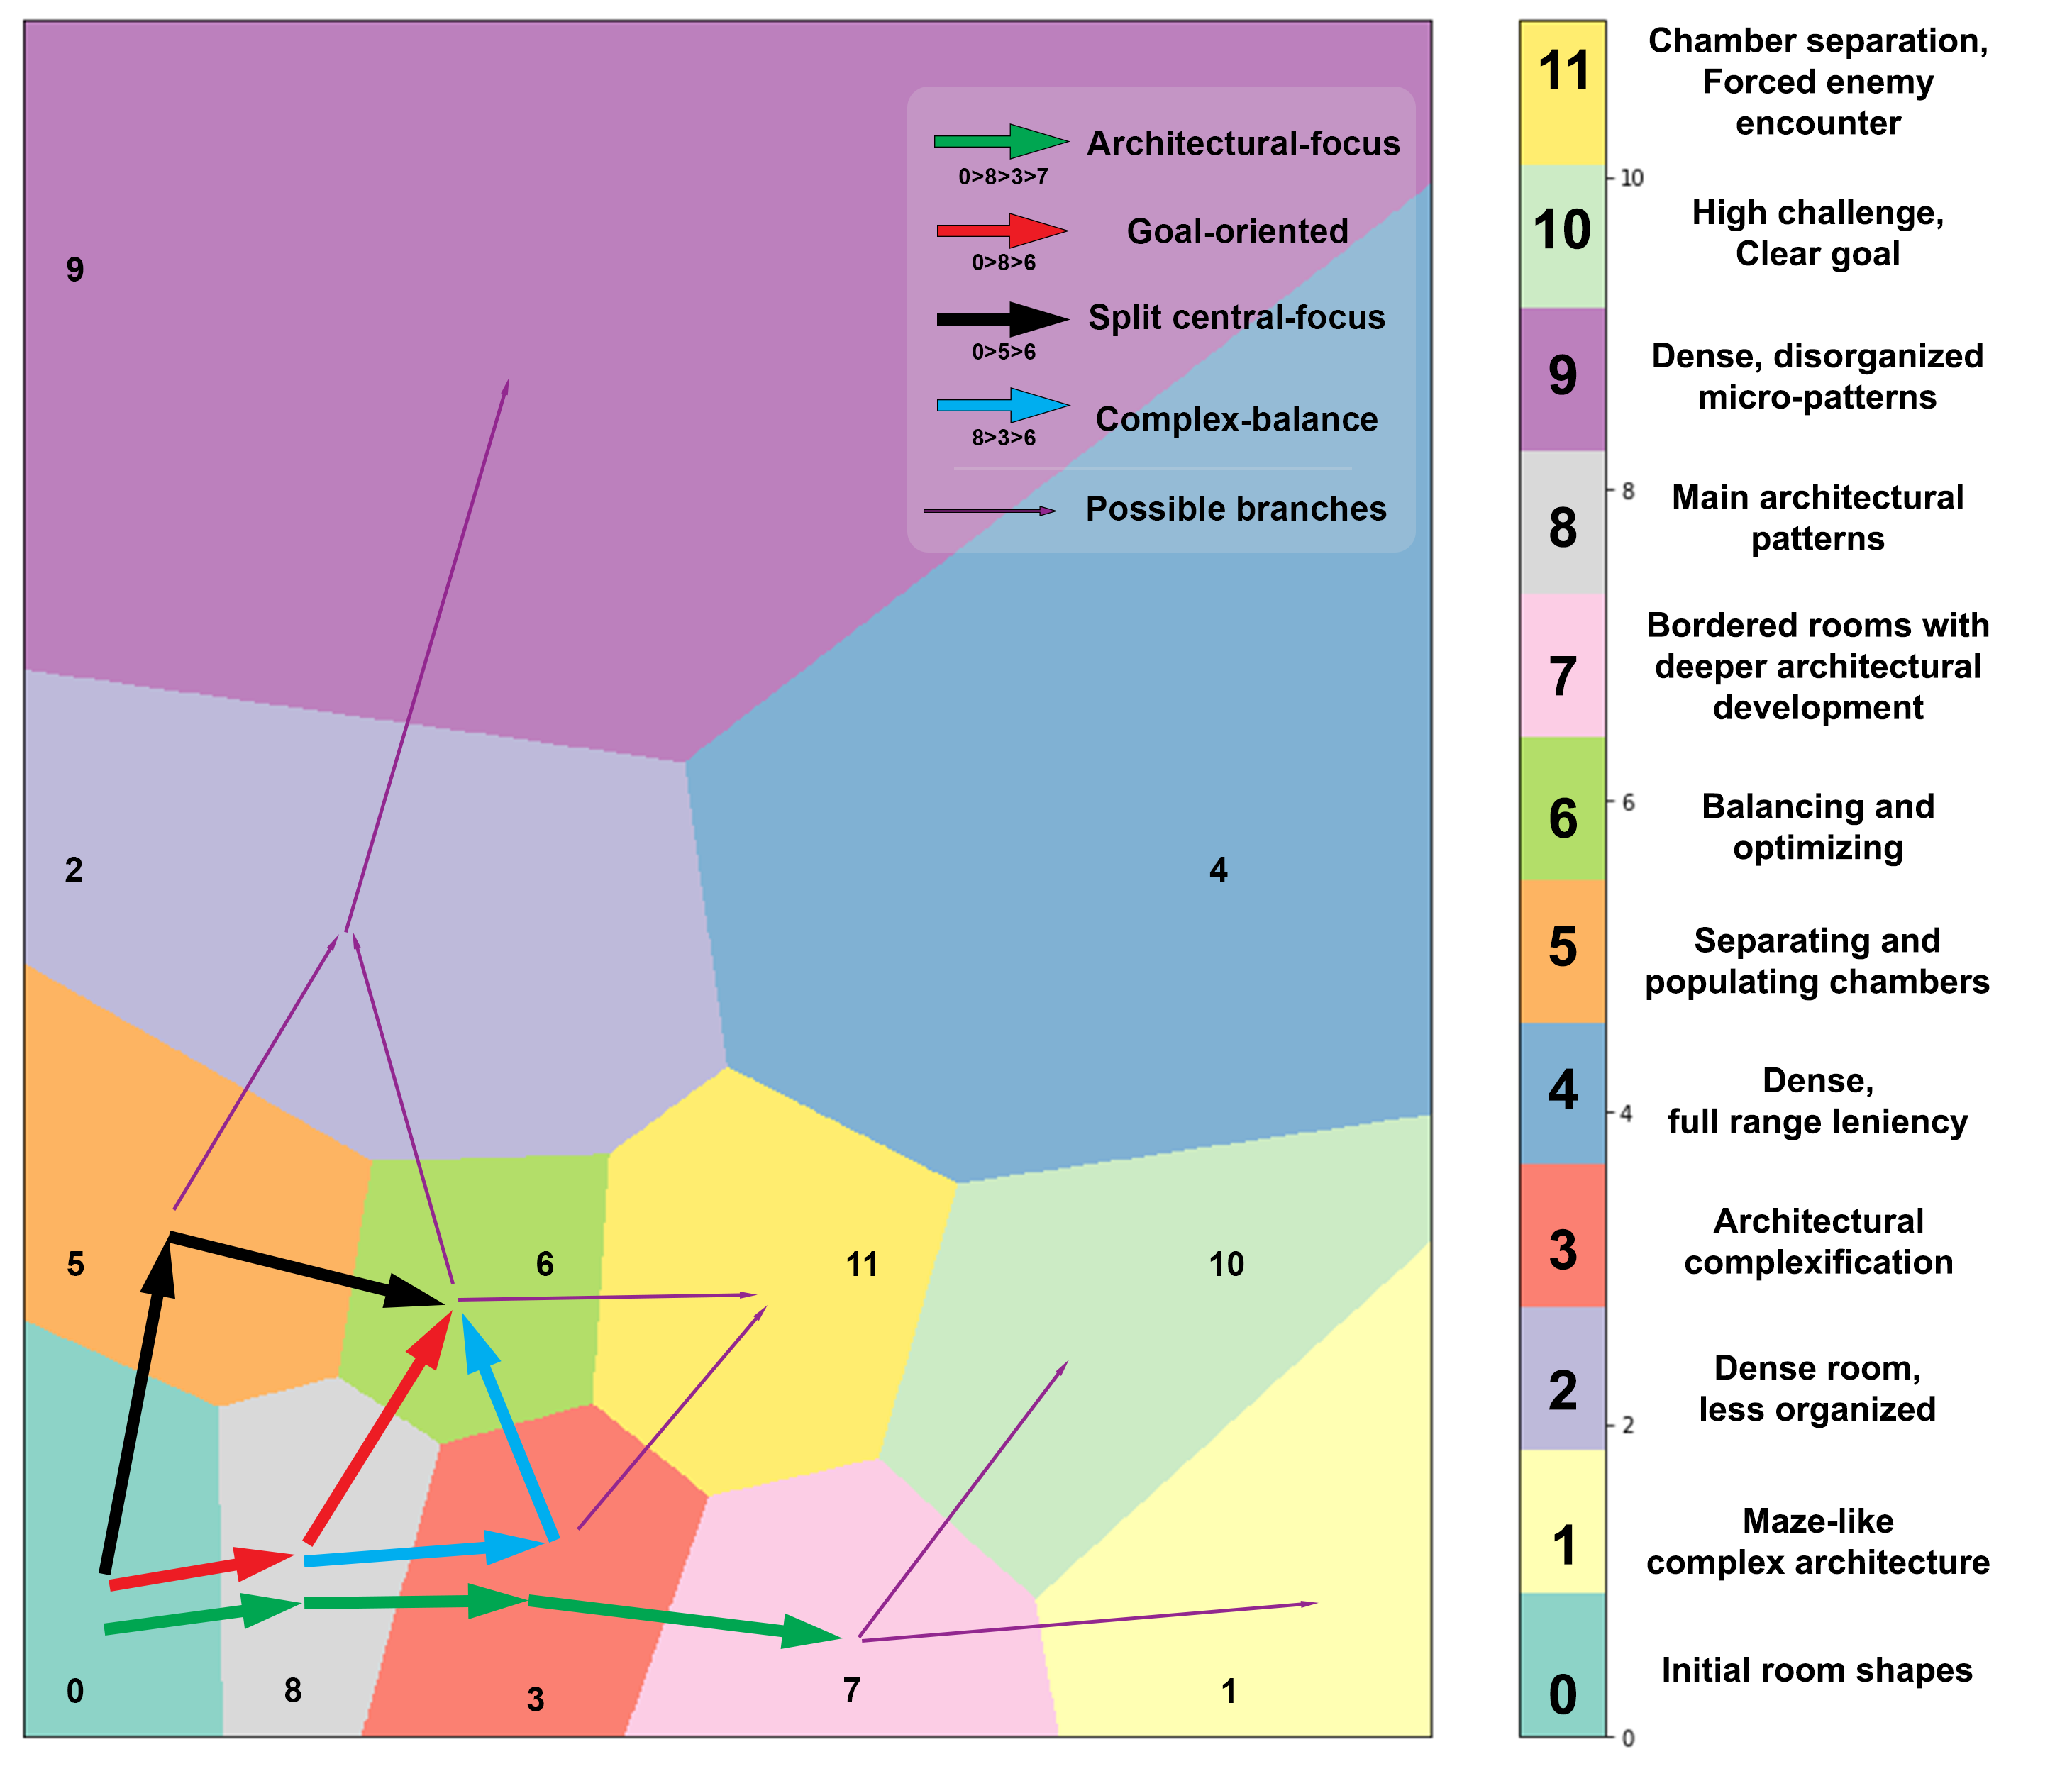
\includegraphics[width=\textwidth]{figures/resulting-paths-FINAL.png}}
\caption{Final and common designer trajectories. With thick arrows it is presented the archetypical paths, calculated using the frequencies of subsequences from $180$ diverse rooms. Each color represent a unique trajectory; with green the \textsc{Architectural-focus}, with red the \textsc{Goal-oriented}, with black the \textsc{Split central-focus}, and with blue the \textsc{Complex-balance}. Finally, thinner purple arrows extending from clusters traversed by the archetypical paths show the multiple possible branches that an archetypical path can deviate or extend to.} \label{p6fig:finalPaths}
\end{figure*}

% \begin{figure*}[t]
% \centerline{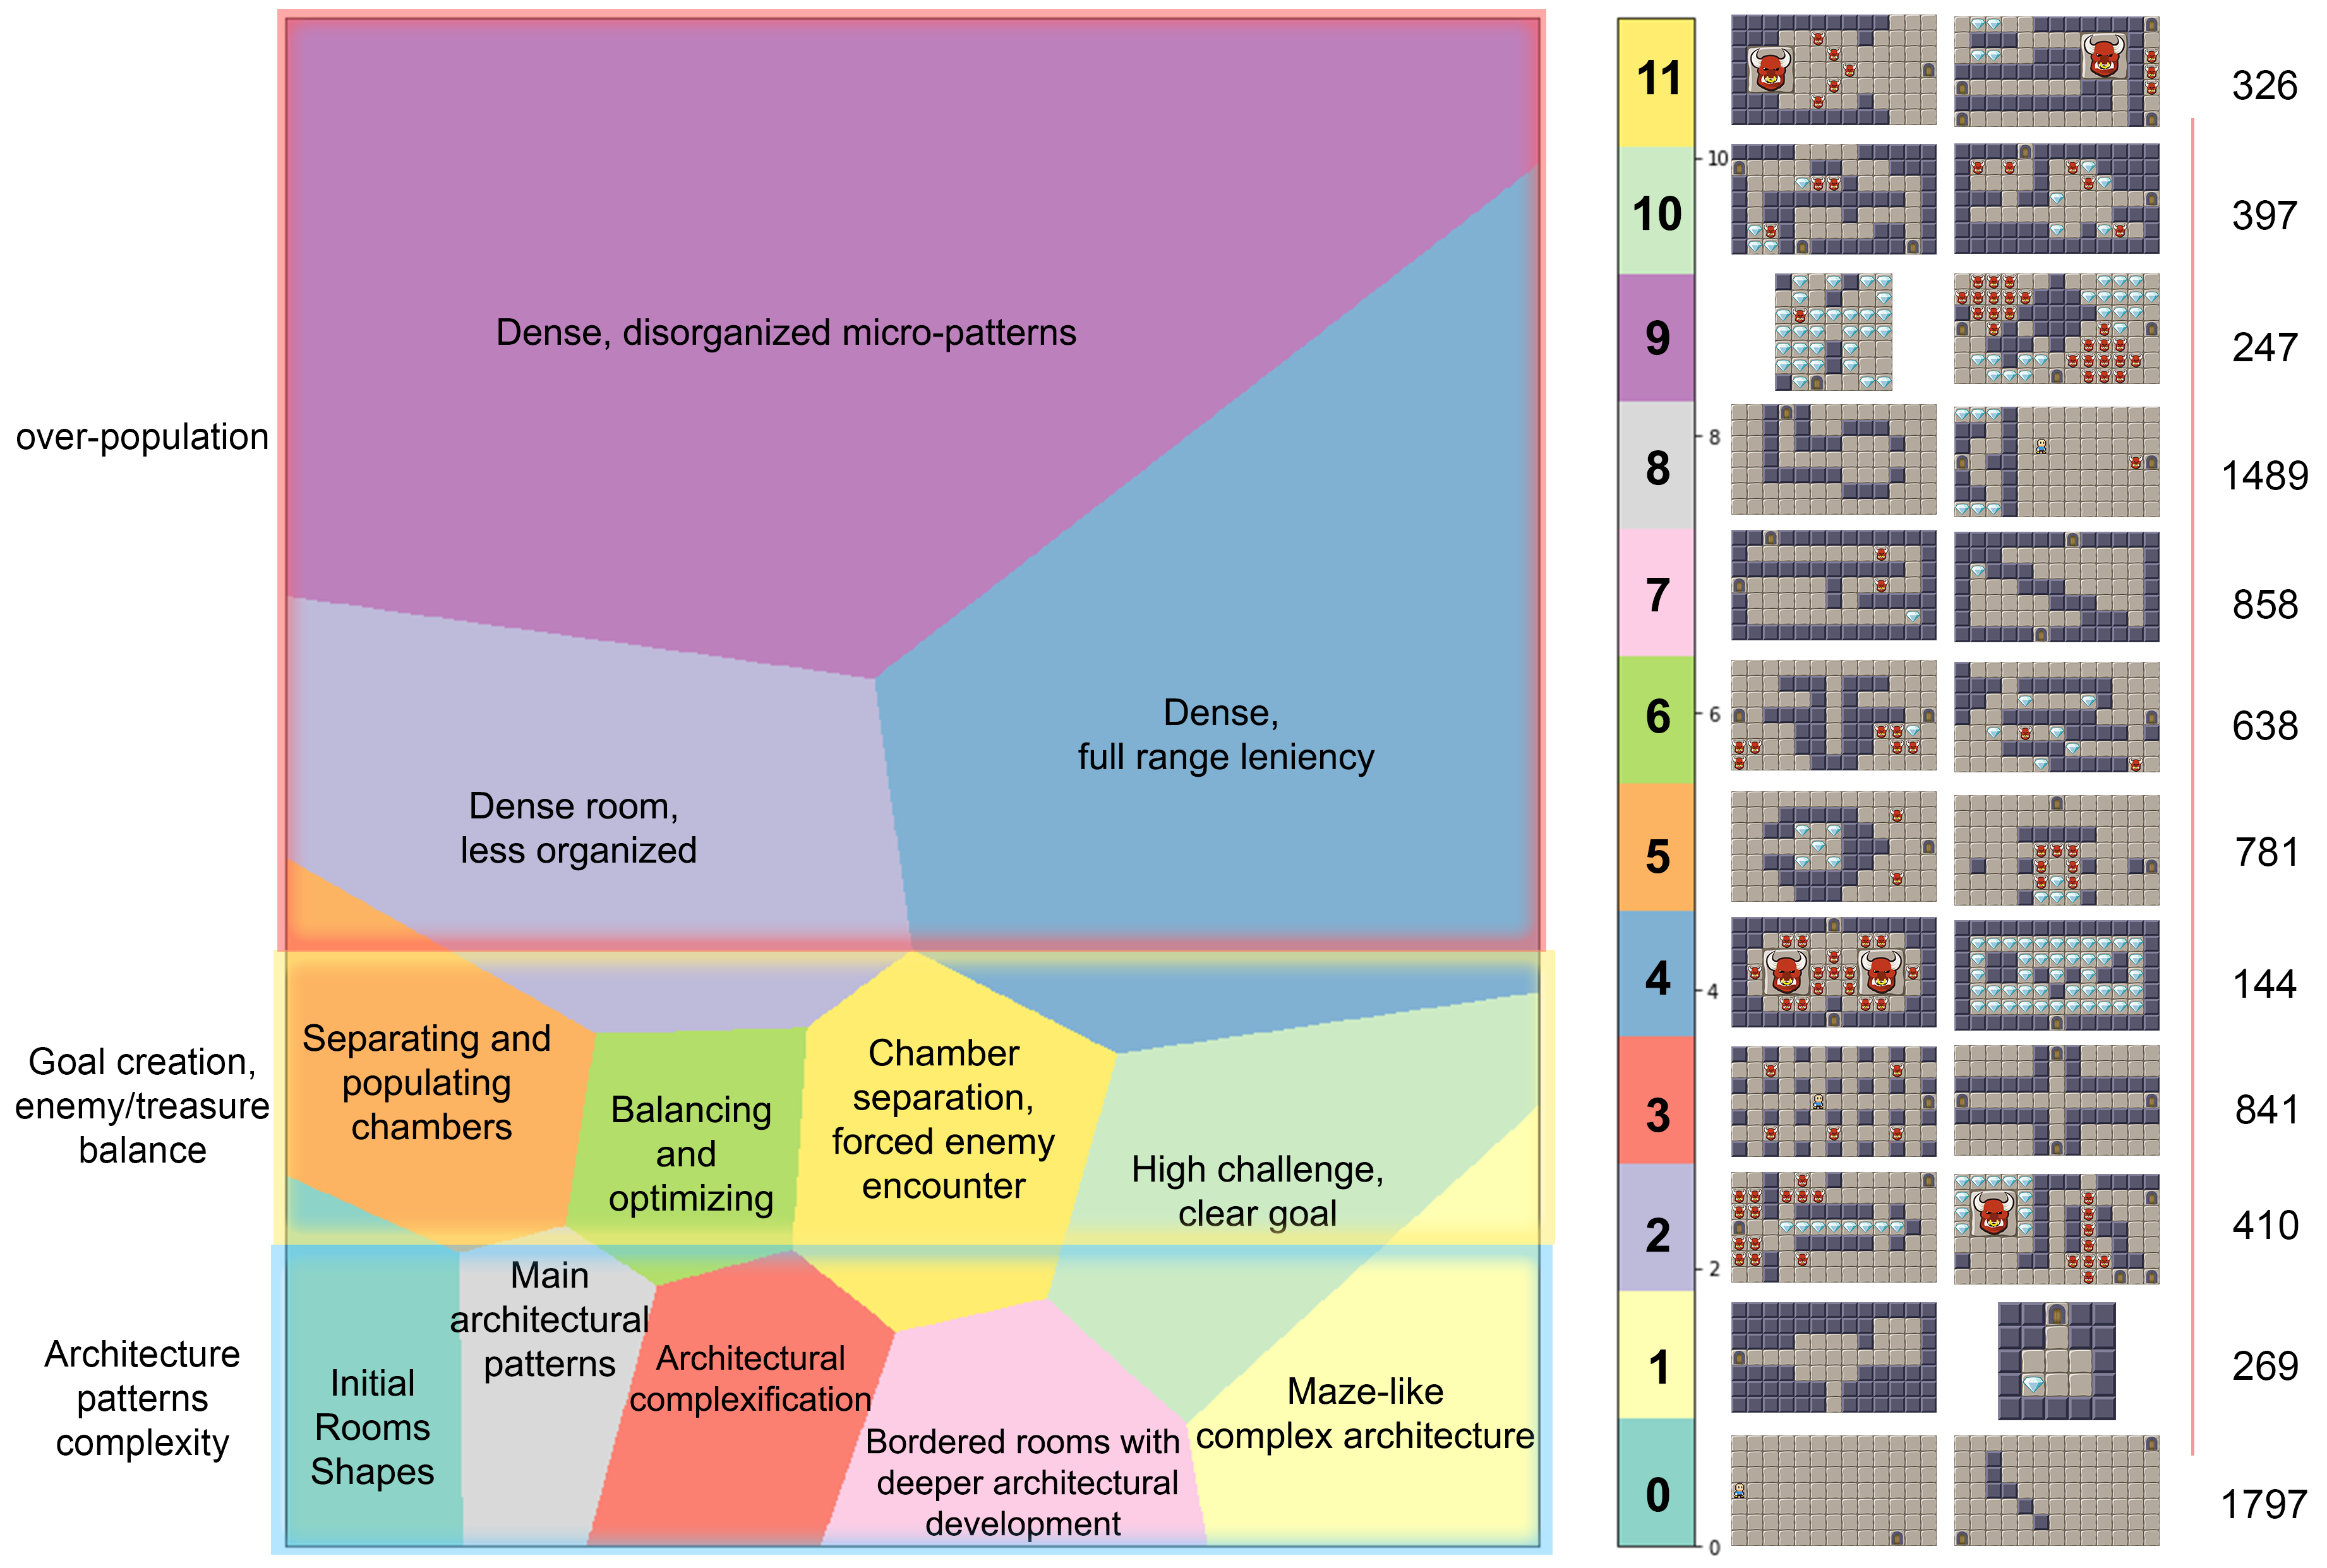
\includegraphics[width=16cm]{figures/final-cluster.png}}
% \caption{Best resulting cluster sets. (a) is K-Means (K=9), and (b) is K-Means (K=12), both are using the \textbf{Tiles} Dataset. While (b) performs slightly worst in the internal indices, when inspecting the qualitative features, it successfully subdivides the main bottom clusters which grants us with more granularity to label and cluster the design process of designers.} \label{p6fig:all-clusters}
% \end{figure*}

% \begin{figure}[t]
% \centerline{\includegraphics[width=8cm]{figures/cluster-figure-updated.png}}
% \caption{Overview of how the design style clustering would be used and integrated into the evaluation of the suggestions provided to the user. %is used and integrates into the evaluation of the suggestions provided to the user.
% } \label{p6fig:cluster}
% \end{figure}

% \begin{figure}[t]
% \centerline{\includegraphics[width=8cm]{figures/all_clusters.png}}
% \caption{All the selected clusters to be labeled and analyzed. In order, each of the clustering approaches correspond to the setups presented in table~\ref{p6table:setups}. (e) Shows extra information on the designs that were clustered together, and which were used to label the respective cluster.} \label{p6fig:all-clusters}
% \end{figure}

% \begin{figure}[b]
% \centerline{\includegraphics[width=8cm]{figures/hand-made-clusters.png}}
% \caption{Example of hand-made room designs used to create the clusters. only (a) and (b) belong to the same clusters} \label{p6fig:handMadeClustered}
% \end{figure}

% \begin{figure*}[t]
% \centerline{\includegraphics[width=18cm]{figures/approach_steps.png}}
% \caption{Rooms at generation $2090$ targeting Number of spatial-patterns (X) and Symmetry (Y). Each cell displays (top-right) the fitness of the optimal individual in its related feasible population. }
% \label{p6figs:approachSteps}
% \end{figure*}

% \begin{figure}[t]
% \centerline{\includegraphics[width=8cm]{figures/cluster-figure-updated.png}}
% \caption{Example of a figure caption.}
% \label{p6fig:implementationClusters}
% \end{figure}
% \subsection{Concepts and Definitions}

%This paper presents an approach and fundamental steps towards the implementation of designer personas: an analysis of designer style clustering to isolate archetypical paths that can be later be used to build ML surrogate models of archetypal designers. Such models would adapt to the dynamic designer during the mixed-initiative creative process by being placed in the solution space, allowing the designer to traverse such space of models as she drifts through the many dimensions of her creative process.

% design archetypes 

Our work draws from ideas, concepts, and definitions introduced by Liapis et al., such as the core designer model loop when using CAD tools, what can be modeled: preferences, style, goals, processes, and their definition, and particularly, the use of designer modeling as an individual or collective model~\citeptenth{p10Liapis2013-designerModel}. We support our approach on the idea of style as a particular type of designer's preference, and that a collective model can be used to form a stable and static design space, which after being interacted with by designers, can be adapted towards them.

% and the idea of style as a particular type of designer's preference.

%. Moreover, Liapis et al. discuss the modeling of style as a type of preference, where each individual designer has peculiarities and characteristics that makes their style recognizable. While we agree with this vision, we 

%Our work draws from many of the ideas and concepts introduced by Liapis et al.~\citeptenth{p10Liapis2013-designerModel}, in relation to style, goals, preferences and design processes of designers. Nevertheless, given the interdisciplinary scope of this system, and the multiple concepts discussed throughout the paper, it is essential to have operational definitions on the different terms used.

%Thus, in this paper, the shared goal is set and defined by the designer with her design, and as she develops, adapts, and changes, the system seeks to adjust its goals to support the designer's work. Furthermore, the aim of this paper is to propose a system that is able to identify the designer's current goal and style to adapt further the system's goals to provide a personalized experience.

\subsubsection{Design Style} \label{sec:designStyle}

%Every designer has a different style when creating content, especially levels, where one might 

% One idea is to train a supervised learning model on traces of other collaborative creation session and try to predict the next step the human would take in the design process. The main problem with this is that people are different, and different creators will want to take different design actions in the same state;

% One way of overcoming this problem could be to change the level of abstraction at which design actions are modeled and predicted. Instead of predicting individual edits, one could identify different styles or phases of the artifact being created, and model how a designer moves from one to another. To put this concretely in the context of designing rooms for a Zelda-like dungeon crawler~\citeptenth{p10tloz}, one could classify room styles depending on whether they were enemy onslaughts, complex wall mazes, treasure puzzles, and so on. One could then train models to recognize which types of rooms a user creates in which order. By clustering sequences of styles or phases we could formulate designer personas as archetypical trajectories through style space, rather than as sequences of individual edits. For example, in the context of creating a dungeon crawler, some designers might start with the outer walls of the rooms and then populate it with NPCs, whereas another type of designer might first sketch the path they would like the player to take from the entrance to the exit and then add parts of the room outside the main path.

There exist many different styles when creating content, especially levels, that designers can create and adapt to accomplish their goals and the experiences they want for players. On a general level, \emph{Design Style} encompasses the creative process from conceptualization, prototyping, reflection, adaptation, especially when following different processes or constraints during collaboration. Taking a more concrete and operational level, \emph{Design Style} can be analyzed as overarching goals that different designers have when creating a dungeon. For instance, dungeons in games such as Zelda\citeptenth{p10tloz} or The Binding of Isaac\citeptenth{p10mcmillen_binding_2011}, represent a particular playing style planned by the designer. In the former, low tempo, exploring the dungeon, and secret rooms define the style of the dungeons, whereas in the latter, high tempo, optimizing time and resources, small rooms, and in general high-challenge define the dungeons. 

While interesting and relevant to understanding the designers' holistic design process and the expected player experience, \emph{Design Style} can also be discussed on an individual room basis. Rooms have their own set of characteristics and styles that can be identified and modeled to understand their design process. Some would prefer to create the room's architecture first to then create the goals within, whereas others would like to place strategic objectives around and then create the architecture around it or alternating between both. Even with such a division, how to reach those design styles is not straightforward and does not require the same strategy, which also shows the preference and style of individual designers. For instance, if the goal is to create a challenge to reach a door, the designer could create a room with a substantial number of enemies, create a concentrated high-challenge in the center of the room, or divide the room into smaller choke areas. Therefore, in this paper, we take a simplified view of \emph{Design Style} and treat it as the style designers follow to create a room, informed by the individual steps each has taken connected to their preferences and goals.

% While this is a simplified view of \emph{Design Style}, we acknowledge that this is a simplified view of \emph{Design Style}, as this could encompass 

% I take some issue with the framing of the paper as being one of modeling someone’s “design style” based only on the sequence of design actions taken as evidenced in snapshots of a design process. To be clear, I think the snapshot approach is a perfectly reasonable one.  But I worry that giving it a term as all-encompassing as “design style” is overpromising, because there is so much about someone’s approach to design that is lost in reducing it to a sequence of partial designs: moments of self-reflection, prototyping and throwing away ideas before moving to new ones, experimentation on paper away from the machine, prior exposure to design and how it informs new design choices, adherence to norms of genre. Obviously these cannot be captured through this approach, nor do they need to be for the work to be valid. Nonetheless, it seems unfair to characterize “design style” as a mere sequence of edit operations.

% I think more precise language would also make clearer what the strengths and limitations of this study are. By naming the aspects of design that are not captured, it makes clear what potential future work there is, how this approach should and should not be applied in other design tools, and the extent to which this work may be generalizable across tools and genres.

% I think this issue also comes up in cluster labeling. Some of the cluster labels refer to properties of room layout (e.g. “maze-like complex architecture”; “dense room”), some to meta-aspects of design (e.g. “high challenge, clear goal”), some to types of actions (e.g. “separating and populating chambers”, “balancing and optimizing”). It seems like it should be possible for a room to fall into two of these labeled clusters simultaneously (e.g. a maze-like room that has many enemies and a clear goal at the end of the maze), and it’s confusing that these are separate clusters. The same is true for other cluster pairs (e.g. “bordered rooms with deeper architectural development” and “dense, full-range leniency” seem like they could co-exist). It’s also not clear how these cluster labels are applied (other than a “qualitative analysis” — but was this done by the research team, or by external experts? how was this evaluated?).


% we use a simplified vision of \emph{Design Style}

% this general level is interesting to udnerstand the designer's holistic design process, there is a need to 

% analyzing the individual rooms gives a

% Every designer has a different style when creating content, especially levels, some would prefer to create the architecture of the room first to them proceed to create the goals within, whereas others would like to place strategic objectives around and then create the architecture around it or alternating between both. Even with such a division, how to reach those design styles is not straightforward and does not require the same strategy, which also shows the preference and style of individual designers. For instance, if the goal is to create challenge to reach a door, the designer could create a room with a substantial amount of enemies, or create a concentrated high-challenge in the center of the room, or divide the room into smaller choke areas.

% Going to a more general level, one could also think of the designs as overarching goals that different designers have when creating the dungeon. For instance, dungeons in games such as Zelda\citeptenth{p10tloz} or The Binding of Isaac\citeptenth{p10mcmillen_binding_2011}, represents a certain playing style planned by the designer. In the former, low tempo, exploring the dungeon, and secret rooms defines the style of the dungeons, whereas in the latter, high tempo, optimizing time and resources, small rooms, and in general high-challenge. While this general level is interesting to udnerstand the designer's holistic design process, there is a need to 

% the whole dungeon represents a certain playing style the design

% One can also think on the designs as a overaching goals that different designers would have, some would luike a high-tempo with smaller rooms and high challenge with minimal rewards while others might prefer the designer to go through more convoluted mazes with many connections to confuse the player and reward the understanding of patterns. While this view is interesting to understand the designer's holistic design process; in this paper we threat Design Style specifically as the style designers follow to create a room, informed by the individual steps each has taken.


% % I think i should discuss 

% % While very discussed, style 

% We can discuss this in both a specific and general level. For adventure and rogue-like games such as Zelda\citeptenth{p10tloz} or The Binding of Isaac\citeptenth{p10mcmillen_binding_2011}, the whole dungeon represents a certain playing style the design  %in-development

% \subsubsection{Designer's Goals}

% Usually, designers' goals are linked to the experiences they want to create for players, however, in a MI-CC tool, the goal is defined as the 

% It is identified as the 
% The designer's goal is defined as the current state of rooms and the set of interactions done in the tool or sequence of steps taken thus far, to reach such a state. Goals by the designer are linked to the addition and strategic placement of enemies and treasures, giving some goal for the player, e.g., forcing the fight with an enemy or allowing the player to avoid the conflict through side paths.



%Specifically, this definition is used as the current goal to be achieve by the designer identified as the sequence of steps taken thus far. Goals by the designer are linked to the addition and strategic placement of enemies and treasures, which gives some type of goal for the player, e.g. force the fight with an enemy or give the opportunity for the player to avoid the conflict through side paths. 

%Moreover, in EDD the designer is tasked to create a dungeon with an unlimited amount of interconnected rooms where each room can be further designed on it's own. When designing the dungeon and the rooms, the designers have the freedom to create the rooms as they want with any goal for the player. For instance, if the goal of the designer is to create a boss room, she might create a room with some narrow corridors that end up in a fight with a boss.



% \subsubsection{System Goals}

% The system goals are defined as the system's approach to support and foster the work of the designer by providing suggestions aligned with her current design or giving assistance, information, visualization, and measurements when needed. In general, when providing suggestions, the system aims at generating rooms among multiple areas of the generative space, simultaneously providing rooms adapted to the designer's goal and different from it. 




%The system's goal is to support the work of the designer by providing assistance, information, and measurement when needed. The system's main feature is the provided suggestions by means of the Interactive Constrained MAP-Elites~\citeptenth{p10Alvarez2020-ICMAPE}. These suggestions adapts to the current room's design by automatically modifying the fitness function in favor of the new features of the room such as enemy and treasure ratios or the balance between corridors and open chambers. Through this suggestions, the goal is to provide possible designs in the generative space for the designer while fostering her creativity by presenting suggestions that might not have been considered by her.




% \subsubsection{Shared Goals}

% The shared goals between the system and the designer are defined as the goals the designer has when creating the dungeon and the individual rooms. Thus, in this paper, the shared goal is set and defined by the designer with her design, and as she develops, adapts, and changes, the system seeks to adjust its goals to support the designer's work. Furthermore, the aim of this paper is to propose a system that is able to identify the designer's current goal and style to adapt further the system's goals to provide a personalized experience.




% \subsubsection{Design Archetypes}
%   %in-development
% Design archetypes or archetypical designer paths are used to describe and represent design processes' paths taken by designers when creating levels 
% This is akin to player archetypes~\citeptenth{p10bartle1996-taxonomy} that partition players into descriptive categories by analyzing their in-game behavior and reactions, design archetypes or archetypical designer paths are used to describe and represent 

% analyzes the behavior of players  partition players into descriptive categories 
\subsection{Concepts and Definitions}

%This paper presents an approach and fundamental steps towards the implementation of designer personas: an analysis of designer style clustering to isolate archetypical paths that can be later be used to build ML surrogate models of archetypal designers. Such models would adapt to the dynamic designer during the mixed-initiative creative process by being placed in the solution space, allowing the designer to traverse such space of models as she drifts through the many dimensions of her creative process.

% design archetypes 

Our work draws from many of the ideas and concepts introduced by Liapis et al.~\citepsixth{p6Liapis2013-designerModel}, in relation to style, goals, preferences and design processes of designers. Nevertheless, given the interdisciplinary scope of this system, and the multiple concepts discuss throughout the paper, it is essential to have operational definitions on the different terms used.

\subsubsection{Design Style} \label{p6sec:designStyle}

%Every designer has a different style when creating content, especially levels, where one might 

% One idea is to train a supervised learning model on traces of other collaborative creation session and try to predict the next step the human would take in the design process. The main problem with this is that people are different, and different creators will want to take different design actions in the same state;

% One way of overcoming this problem could be to change the level of abstraction at which design actions are modeled and predicted. Instead of predicting individual edits, one could identify different styles or phases of the artifact being created, and model how a designer moves from one to another. To put this concretely in the context of designing rooms for a Zelda-like dungeon crawler~\citepsixth{p6tloz}, one could classify room styles depending on whether they were enemy onslaughts, complex wall mazes, treasure puzzles, and so on. One could then train models to recognize which types of rooms a user creates in which order. By clustering sequences of styles or phases we could formulate designer personas as archetypical trajectories through style space, rather than as sequences of individual edits. For example, in the context of creating a dungeon crawler, some designers might start with the outer walls of the rooms and then populate it with NPCs, whereas another type of designer might first sketch the path they would like the player to take from the entrance to the exit and then add parts of the room outside the main path.

There exist many different styles when creating content, especially levels, that designers can create and adapt to accomplish their goals and the experiences they want for players. On a general level, \emph{Design Style} can be analyzed as overarching goals that different designers have when creating a dungeon. For instance, dungeons in games such as Zelda\citepsixth{p6tloz} or The Binding of Isaac\citepsixth{p6mcmillen_binding_2011}, represent a particular playing style planned by the designer. In the former, low tempo, exploring the dungeon, and secret rooms define the style of the dungeons, whereas in the latter, high tempo, optimizing time and resources, small rooms, and in general high-challenge define the dungeons. 

While interesting and relevant to understand the designers' holistic design process and the expected player experience, \emph{Design Style} can also be discussed from an individual room basis. Rooms have their own set of characteristics and styles that can be identified and modeled to understand their design process. Some would prefer to create the architecture of the room first to then create the goals within, whereas others would like to place strategic objectives around and then create the architecture around it or alternating between both. Even with such a division, how to reach those design styles is not straightforward and does not require the same strategy, which also shows the preference and style of individual designers. For instance, if the goal is to create a challenge to reach a door, the designer could create a room with a substantial amount of enemies, or create a concentrated high-challenge in the center of the room, or divide the room into smaller choke areas. Therefore, in this paper, we treat \emph{Design Style} as the style designers follow to create a room, informed by the individual steps each has taken connected to their preferences and goals.

% this general level is interesting to udnerstand the designer's holistic design process, there is a need to 

% analyzing the individual rooms gives a

% Every designer has a different style when creating content, especially levels, some would prefer to create the architecture of the room first to them proceed to create the goals within, whereas others would like to place strategic objectives around and then create the architecture around it or alternating between both. Even with such a division, how to reach those design styles is not straightforward and does not require the same strategy, which also shows the preference and style of individual designers. For instance, if the goal is to create challenge to reach a door, the designer could create a room with a substantial amount of enemies, or create a concentrated high-challenge in the center of the room, or divide the room into smaller choke areas.

% Going to a more general level, one could also think of the designs as overarching goals that different designers have when creating the dungeon. For instance, dungeons in games such as Zelda\citepsixth{p6tloz} or The Binding of Isaac\citepsixth{p6mcmillen_binding_2011}, represents a certain playing style planned by the designer. In the former, low tempo, exploring the dungeon, and secret rooms defines the style of the dungeons, whereas in the latter, high tempo, optimizing time and resources, small rooms, and in general high-challenge. While this general level is interesting to udnerstand the designer's holistic design process, there is a need to 

% the whole dungeon represents a certain playing style the design

% One can also think on the designs as a overaching goals that different designers would have, some would luike a high-tempo with smaller rooms and high challenge with minimal rewards while others might prefer the designer to go through more convoluted mazes with many connections to confuse the player and reward the understanding of patterns. While this view is interesting to understand the designer's holistic design process; in this paper we threat Design Style specifically as the style designers follow to create a room, informed by the individual steps each has taken.


% % I think i should discuss 

% % While very discussed, style 

% We can discuss this in both a specific and general level. For adventure and rogue-like games such as Zelda\citepsixth{p6tloz} or The Binding of Isaac\citepsixth{p6mcmillen_binding_2011}, the whole dungeon represents a certain playing style the design  %in-development

\subsubsection{Designer's Goals}

% Usually, designers' goals are linked to the experiences they want to create for players, however, in a MI-CC tool, the goal is defined as the 

% It is identified as the 
The designer's goal is defined as the current state of rooms and the set of interactions done in the tool or sequence of steps taken thus far, to reach such a state. Goals by the designer are linked to the addition and strategic placement of enemies and treasures, giving some goal for the player, e.g., forcing the fight with an enemy or allowing the player to avoid the conflict through side paths.

%Specifically, this definition is used as the current goal to be achieve by the designer identified as the sequence of steps taken thus far. Goals by the designer are linked to the addition and strategic placement of enemies and treasures, which gives some type of goal for the player, e.g. force the fight with an enemy or give the opportunity for the player to avoid the conflict through side paths. 

%Moreover, in EDD the designer is tasked to create a dungeon with an unlimited amount of interconnected rooms where each room can be further designed on it's own. When designing the dungeon and the rooms, the designers have the freedom to create the rooms as they want with any goal for the player. For instance, if the goal of the designer is to create a boss room, she might create a room with some narrow corridors that end up in a fight with a boss.

\subsubsection{System Goals}

The system goals are defined as the system's approach to support and foster the work of the designer by providing suggestions aligned with her current design or giving assistance, information, visualization, and measurements when needed. In general, when providing suggestions, the system aims at generating rooms among multiple areas of the generative space, simultaneously providing rooms adapted to the designer's goal and different from it. 

%The system's goal is to support the work of the designer by providing assistance, information, and measurement when needed. The system's main feature is the provided suggestions by means of the Interactive Constrained MAP-Elites~\citepsixth{p6Alvarez2020-ICMAPE}. These suggestions adapts to the current room's design by automatically modifying the fitness function in favor of the new features of the room such as enemy and treasure ratios or the balance between corridors and open chambers. Through this suggestions, the goal is to provide possible designs in the generative space for the designer while fostering her creativity by presenting suggestions that might not have been considered by her.

\subsubsection{Shared Goals}

The shared goals between the system and the designer are defined as the goals the designer has when creating the dungeon and the individual rooms. Thus, in this paper, the shared goal is set and defined by the designer with her design, and as she develops, adapts, and changes, the system seeks to adjust its goals to support the designer's work. Furthermore, the aim of this paper is to propose a system that is able to identify the designer's current goal and style to adapt further the system's goals to provide a personalized experience.

% \subsubsection{Design Archetypes}
%   %in-development
% Design archetypes or archetypical designer paths are used to describe and represent design processes' paths taken by designers when creating levels 
% This is akin to player archetypes~\citepsixth{p6bartle1996-taxonomy} that partition players into descriptive categories by analyzing their in-game behavior and reactions, design archetypes or archetypical designer paths are used to describe and represent 

% analyzes the behavior of players  partition players into descriptive categories 
% \subsection{Concepts and Definitions}

%This paper presents an approach and fundamental steps towards the implementation of designer personas: an analysis of designer style clustering to isolate archetypical paths that can be later be used to build ML surrogate models of archetypal designers. Such models would adapt to the dynamic designer during the mixed-initiative creative process by being placed in the solution space, allowing the designer to traverse such space of models as she drifts through the many dimensions of her creative process.

% design archetypes 

Our work draws from ideas, concepts, and definitions introduced by Liapis et al., such as the core designer model loop when using CAD tools, what can be modeled: preferences, style, goals, processes, and their definition, and particularly, the use of designer modeling as an individual or collective model~\citeptenth{p10Liapis2013-designerModel}. We support our approach on the idea of style as a particular type of designer's preference, and that a collective model can be used to form a stable and static design space, which after being interacted with by designers, can be adapted towards them.

% and the idea of style as a particular type of designer's preference.

%. Moreover, Liapis et al. discuss the modeling of style as a type of preference, where each individual designer has peculiarities and characteristics that makes their style recognizable. While we agree with this vision, we 

%Our work draws from many of the ideas and concepts introduced by Liapis et al.~\citeptenth{p10Liapis2013-designerModel}, in relation to style, goals, preferences and design processes of designers. Nevertheless, given the interdisciplinary scope of this system, and the multiple concepts discussed throughout the paper, it is essential to have operational definitions on the different terms used.

%Thus, in this paper, the shared goal is set and defined by the designer with her design, and as she develops, adapts, and changes, the system seeks to adjust its goals to support the designer's work. Furthermore, the aim of this paper is to propose a system that is able to identify the designer's current goal and style to adapt further the system's goals to provide a personalized experience.

\subsubsection{Design Style} \label{sec:designStyle}

%Every designer has a different style when creating content, especially levels, where one might 

% One idea is to train a supervised learning model on traces of other collaborative creation session and try to predict the next step the human would take in the design process. The main problem with this is that people are different, and different creators will want to take different design actions in the same state;

% One way of overcoming this problem could be to change the level of abstraction at which design actions are modeled and predicted. Instead of predicting individual edits, one could identify different styles or phases of the artifact being created, and model how a designer moves from one to another. To put this concretely in the context of designing rooms for a Zelda-like dungeon crawler~\citeptenth{p10tloz}, one could classify room styles depending on whether they were enemy onslaughts, complex wall mazes, treasure puzzles, and so on. One could then train models to recognize which types of rooms a user creates in which order. By clustering sequences of styles or phases we could formulate designer personas as archetypical trajectories through style space, rather than as sequences of individual edits. For example, in the context of creating a dungeon crawler, some designers might start with the outer walls of the rooms and then populate it with NPCs, whereas another type of designer might first sketch the path they would like the player to take from the entrance to the exit and then add parts of the room outside the main path.

There exist many different styles when creating content, especially levels, that designers can create and adapt to accomplish their goals and the experiences they want for players. On a general level, \emph{Design Style} encompasses the creative process from conceptualization, prototyping, reflection, adaptation, especially when following different processes or constraints during collaboration. Taking a more concrete and operational level, \emph{Design Style} can be analyzed as overarching goals that different designers have when creating a dungeon. For instance, dungeons in games such as Zelda\citeptenth{p10tloz} or The Binding of Isaac\citeptenth{p10mcmillen_binding_2011}, represent a particular playing style planned by the designer. In the former, low tempo, exploring the dungeon, and secret rooms define the style of the dungeons, whereas in the latter, high tempo, optimizing time and resources, small rooms, and in general high-challenge define the dungeons. 

While interesting and relevant to understanding the designers' holistic design process and the expected player experience, \emph{Design Style} can also be discussed on an individual room basis. Rooms have their own set of characteristics and styles that can be identified and modeled to understand their design process. Some would prefer to create the room's architecture first to then create the goals within, whereas others would like to place strategic objectives around and then create the architecture around it or alternating between both. Even with such a division, how to reach those design styles is not straightforward and does not require the same strategy, which also shows the preference and style of individual designers. For instance, if the goal is to create a challenge to reach a door, the designer could create a room with a substantial number of enemies, create a concentrated high-challenge in the center of the room, or divide the room into smaller choke areas. Therefore, in this paper, we take a simplified view of \emph{Design Style} and treat it as the style designers follow to create a room, informed by the individual steps each has taken connected to their preferences and goals.

% While this is a simplified view of \emph{Design Style}, we acknowledge that this is a simplified view of \emph{Design Style}, as this could encompass 

% I take some issue with the framing of the paper as being one of modeling someone’s “design style” based only on the sequence of design actions taken as evidenced in snapshots of a design process. To be clear, I think the snapshot approach is a perfectly reasonable one.  But I worry that giving it a term as all-encompassing as “design style” is overpromising, because there is so much about someone’s approach to design that is lost in reducing it to a sequence of partial designs: moments of self-reflection, prototyping and throwing away ideas before moving to new ones, experimentation on paper away from the machine, prior exposure to design and how it informs new design choices, adherence to norms of genre. Obviously these cannot be captured through this approach, nor do they need to be for the work to be valid. Nonetheless, it seems unfair to characterize “design style” as a mere sequence of edit operations.

% I think more precise language would also make clearer what the strengths and limitations of this study are. By naming the aspects of design that are not captured, it makes clear what potential future work there is, how this approach should and should not be applied in other design tools, and the extent to which this work may be generalizable across tools and genres.

% I think this issue also comes up in cluster labeling. Some of the cluster labels refer to properties of room layout (e.g. “maze-like complex architecture”; “dense room”), some to meta-aspects of design (e.g. “high challenge, clear goal”), some to types of actions (e.g. “separating and populating chambers”, “balancing and optimizing”). It seems like it should be possible for a room to fall into two of these labeled clusters simultaneously (e.g. a maze-like room that has many enemies and a clear goal at the end of the maze), and it’s confusing that these are separate clusters. The same is true for other cluster pairs (e.g. “bordered rooms with deeper architectural development” and “dense, full-range leniency” seem like they could co-exist). It’s also not clear how these cluster labels are applied (other than a “qualitative analysis” — but was this done by the research team, or by external experts? how was this evaluated?).


% we use a simplified vision of \emph{Design Style}

% this general level is interesting to udnerstand the designer's holistic design process, there is a need to 

% analyzing the individual rooms gives a

% Every designer has a different style when creating content, especially levels, some would prefer to create the architecture of the room first to them proceed to create the goals within, whereas others would like to place strategic objectives around and then create the architecture around it or alternating between both. Even with such a division, how to reach those design styles is not straightforward and does not require the same strategy, which also shows the preference and style of individual designers. For instance, if the goal is to create challenge to reach a door, the designer could create a room with a substantial amount of enemies, or create a concentrated high-challenge in the center of the room, or divide the room into smaller choke areas.

% Going to a more general level, one could also think of the designs as overarching goals that different designers have when creating the dungeon. For instance, dungeons in games such as Zelda\citeptenth{p10tloz} or The Binding of Isaac\citeptenth{p10mcmillen_binding_2011}, represents a certain playing style planned by the designer. In the former, low tempo, exploring the dungeon, and secret rooms defines the style of the dungeons, whereas in the latter, high tempo, optimizing time and resources, small rooms, and in general high-challenge. While this general level is interesting to udnerstand the designer's holistic design process, there is a need to 

% the whole dungeon represents a certain playing style the design

% One can also think on the designs as a overaching goals that different designers would have, some would luike a high-tempo with smaller rooms and high challenge with minimal rewards while others might prefer the designer to go through more convoluted mazes with many connections to confuse the player and reward the understanding of patterns. While this view is interesting to understand the designer's holistic design process; in this paper we threat Design Style specifically as the style designers follow to create a room, informed by the individual steps each has taken.


% % I think i should discuss 

% % While very discussed, style 

% We can discuss this in both a specific and general level. For adventure and rogue-like games such as Zelda\citeptenth{p10tloz} or The Binding of Isaac\citeptenth{p10mcmillen_binding_2011}, the whole dungeon represents a certain playing style the design  %in-development

% \subsubsection{Designer's Goals}

% Usually, designers' goals are linked to the experiences they want to create for players, however, in a MI-CC tool, the goal is defined as the 

% It is identified as the 
% The designer's goal is defined as the current state of rooms and the set of interactions done in the tool or sequence of steps taken thus far, to reach such a state. Goals by the designer are linked to the addition and strategic placement of enemies and treasures, giving some goal for the player, e.g., forcing the fight with an enemy or allowing the player to avoid the conflict through side paths.



%Specifically, this definition is used as the current goal to be achieve by the designer identified as the sequence of steps taken thus far. Goals by the designer are linked to the addition and strategic placement of enemies and treasures, which gives some type of goal for the player, e.g. force the fight with an enemy or give the opportunity for the player to avoid the conflict through side paths. 

%Moreover, in EDD the designer is tasked to create a dungeon with an unlimited amount of interconnected rooms where each room can be further designed on it's own. When designing the dungeon and the rooms, the designers have the freedom to create the rooms as they want with any goal for the player. For instance, if the goal of the designer is to create a boss room, she might create a room with some narrow corridors that end up in a fight with a boss.



% \subsubsection{System Goals}

% The system goals are defined as the system's approach to support and foster the work of the designer by providing suggestions aligned with her current design or giving assistance, information, visualization, and measurements when needed. In general, when providing suggestions, the system aims at generating rooms among multiple areas of the generative space, simultaneously providing rooms adapted to the designer's goal and different from it. 




%The system's goal is to support the work of the designer by providing assistance, information, and measurement when needed. The system's main feature is the provided suggestions by means of the Interactive Constrained MAP-Elites~\citeptenth{p10Alvarez2020-ICMAPE}. These suggestions adapts to the current room's design by automatically modifying the fitness function in favor of the new features of the room such as enemy and treasure ratios or the balance between corridors and open chambers. Through this suggestions, the goal is to provide possible designs in the generative space for the designer while fostering her creativity by presenting suggestions that might not have been considered by her.




% \subsubsection{Shared Goals}

% The shared goals between the system and the designer are defined as the goals the designer has when creating the dungeon and the individual rooms. Thus, in this paper, the shared goal is set and defined by the designer with her design, and as she develops, adapts, and changes, the system seeks to adjust its goals to support the designer's work. Furthermore, the aim of this paper is to propose a system that is able to identify the designer's current goal and style to adapt further the system's goals to provide a personalized experience.




% \subsubsection{Design Archetypes}
%   %in-development
% Design archetypes or archetypical designer paths are used to describe and represent design processes' paths taken by designers when creating levels 
% This is akin to player archetypes~\citeptenth{p10bartle1996-taxonomy} that partition players into descriptive categories by analyzing their in-game behavior and reactions, design archetypes or archetypical designer paths are used to describe and represent 

% analyzes the behavior of players  partition players into descriptive categories 
\subsection{Designer Personas} \label{p6section:results}

%We  trained  3  models  for  each  representation  and  problem configuration. To analyze these models, we collected 40 generated levels for each model.  To generate the levels, 40 different random level layouts were generated, the models were then tasked with modifying these random layouts into good levels.   We  analyzed  the  final  modified  levels  using  different change percentages, ranging from0%to100%, where thepercentage represents the fraction of tiles the agent is allowedto change during inference

%To understand the typical progress of designers and validate the clustering, we visualize how typical design sessions traverse the various clusters. These trajectories  are  then  clustered  to  find  a  small  handful of designer personas.

\begin{figure*}[t]
    \centering
     \subfloat[\textsc{Architectural-focus}\label{p6subfig-1:dummy}]{%
       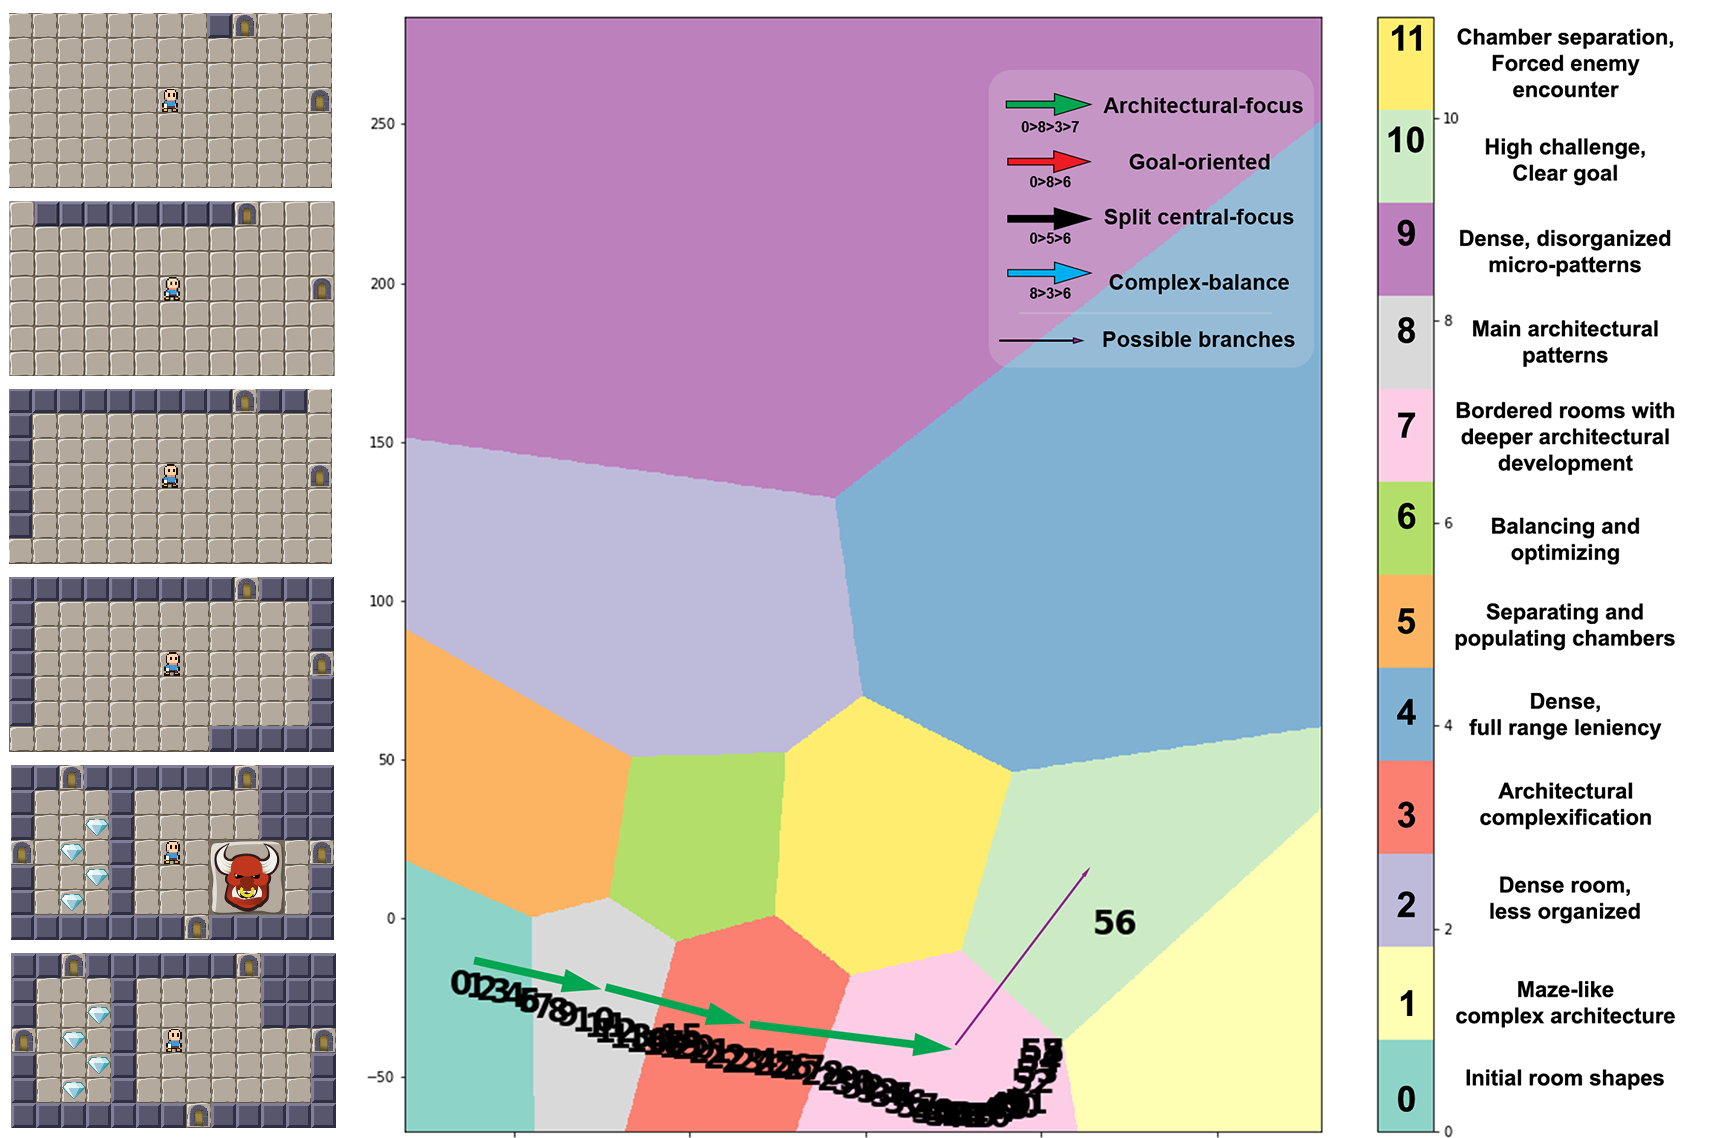
\includegraphics[width=0.45\textwidth]{figures/1.png}
     }
     \hfill
     \subfloat[\textsc{Goal-oriented}\label{p6subfig-2:dummy}]{%
       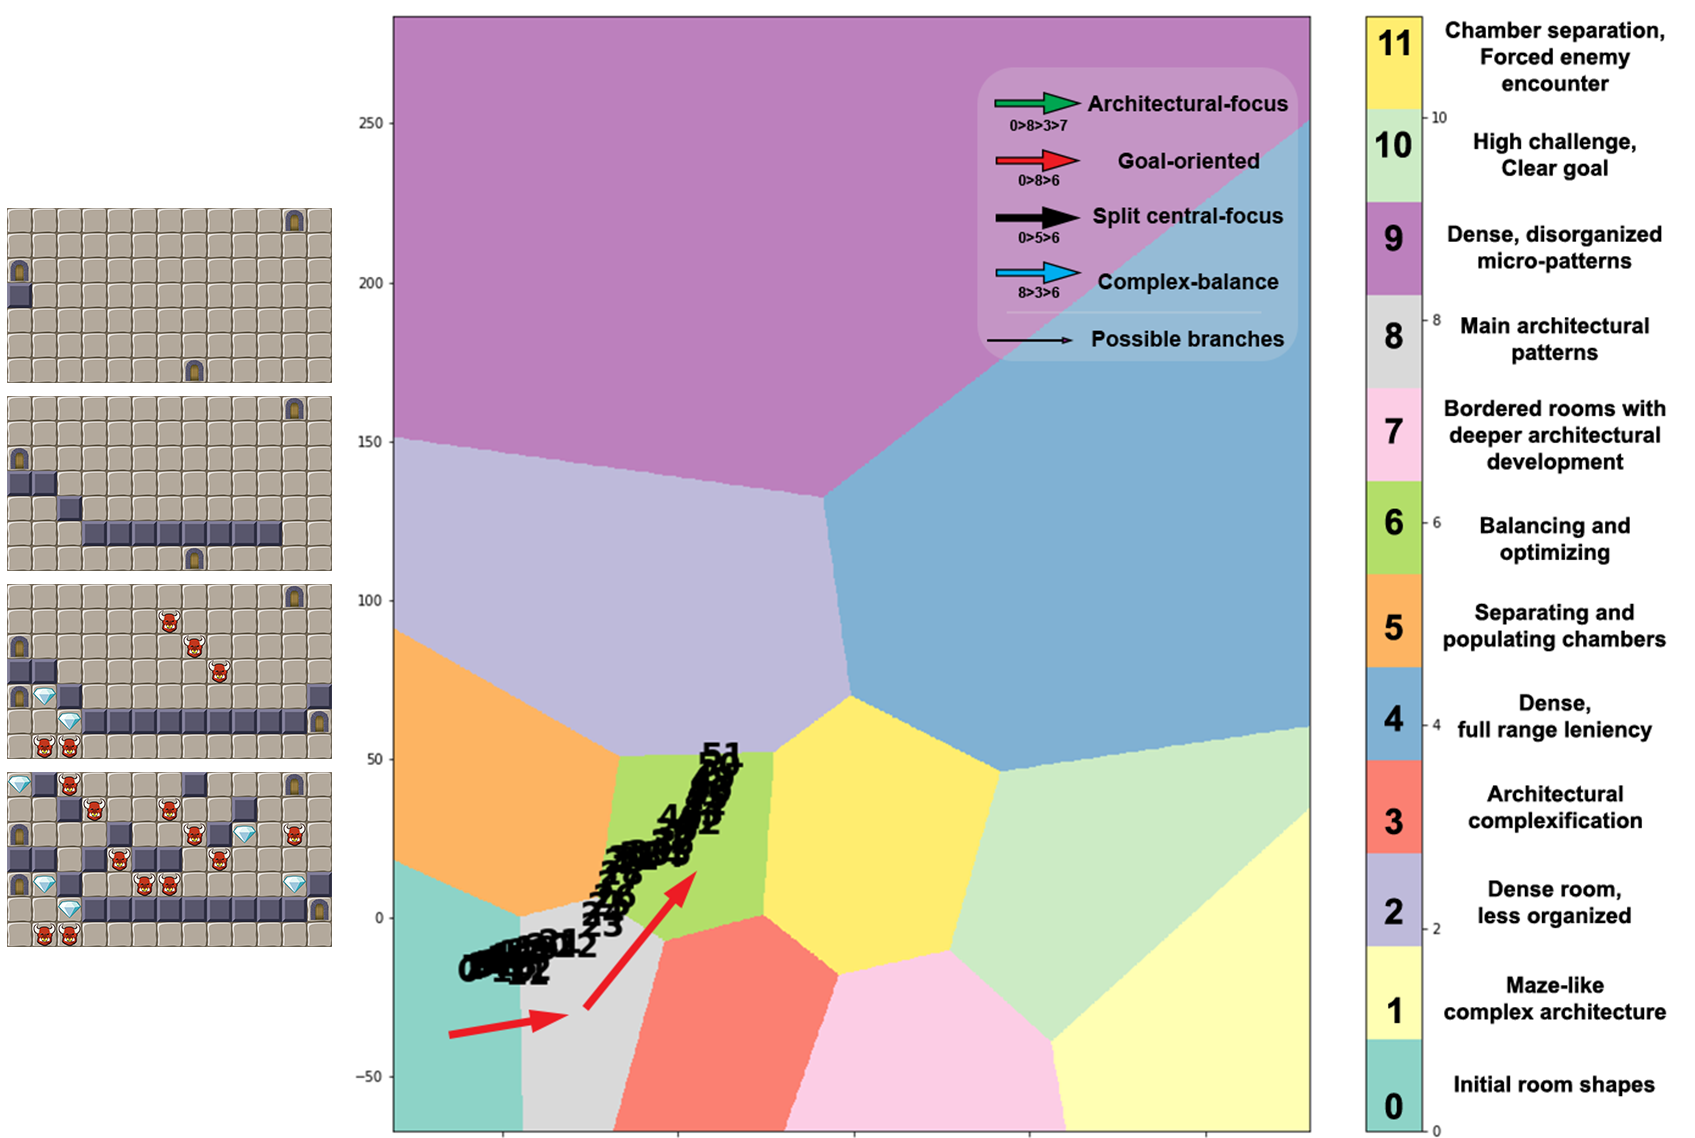
\includegraphics[width=0.45\textwidth]{figures/2.png}
     }\hfill
    %  \medskip
     \subfloat[\textsc{Split central-focus}\label{p6subfig-3:dummy}]{%
       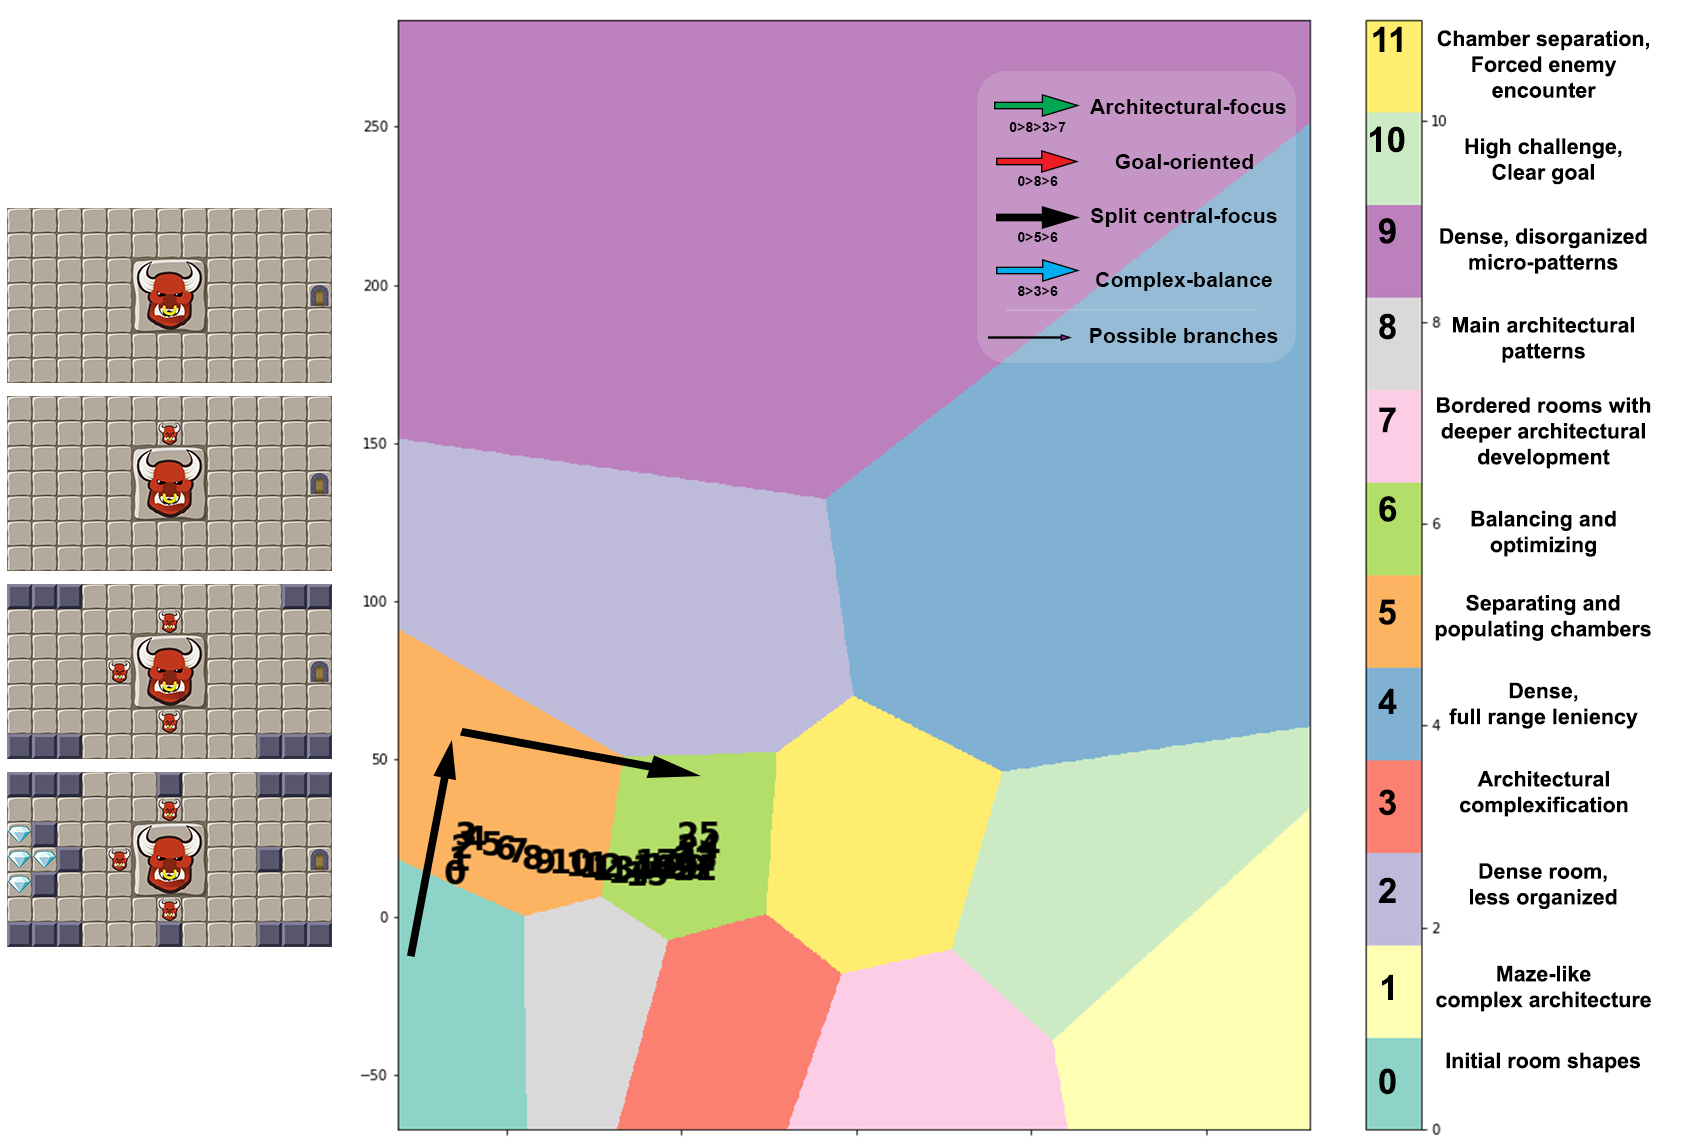
\includegraphics[width=0.45\textwidth]{figures/3.png}
     }
     \hfill
     \subfloat[\textsc{Complex-balance}\label{p6subfig-4:dummy}]{%
       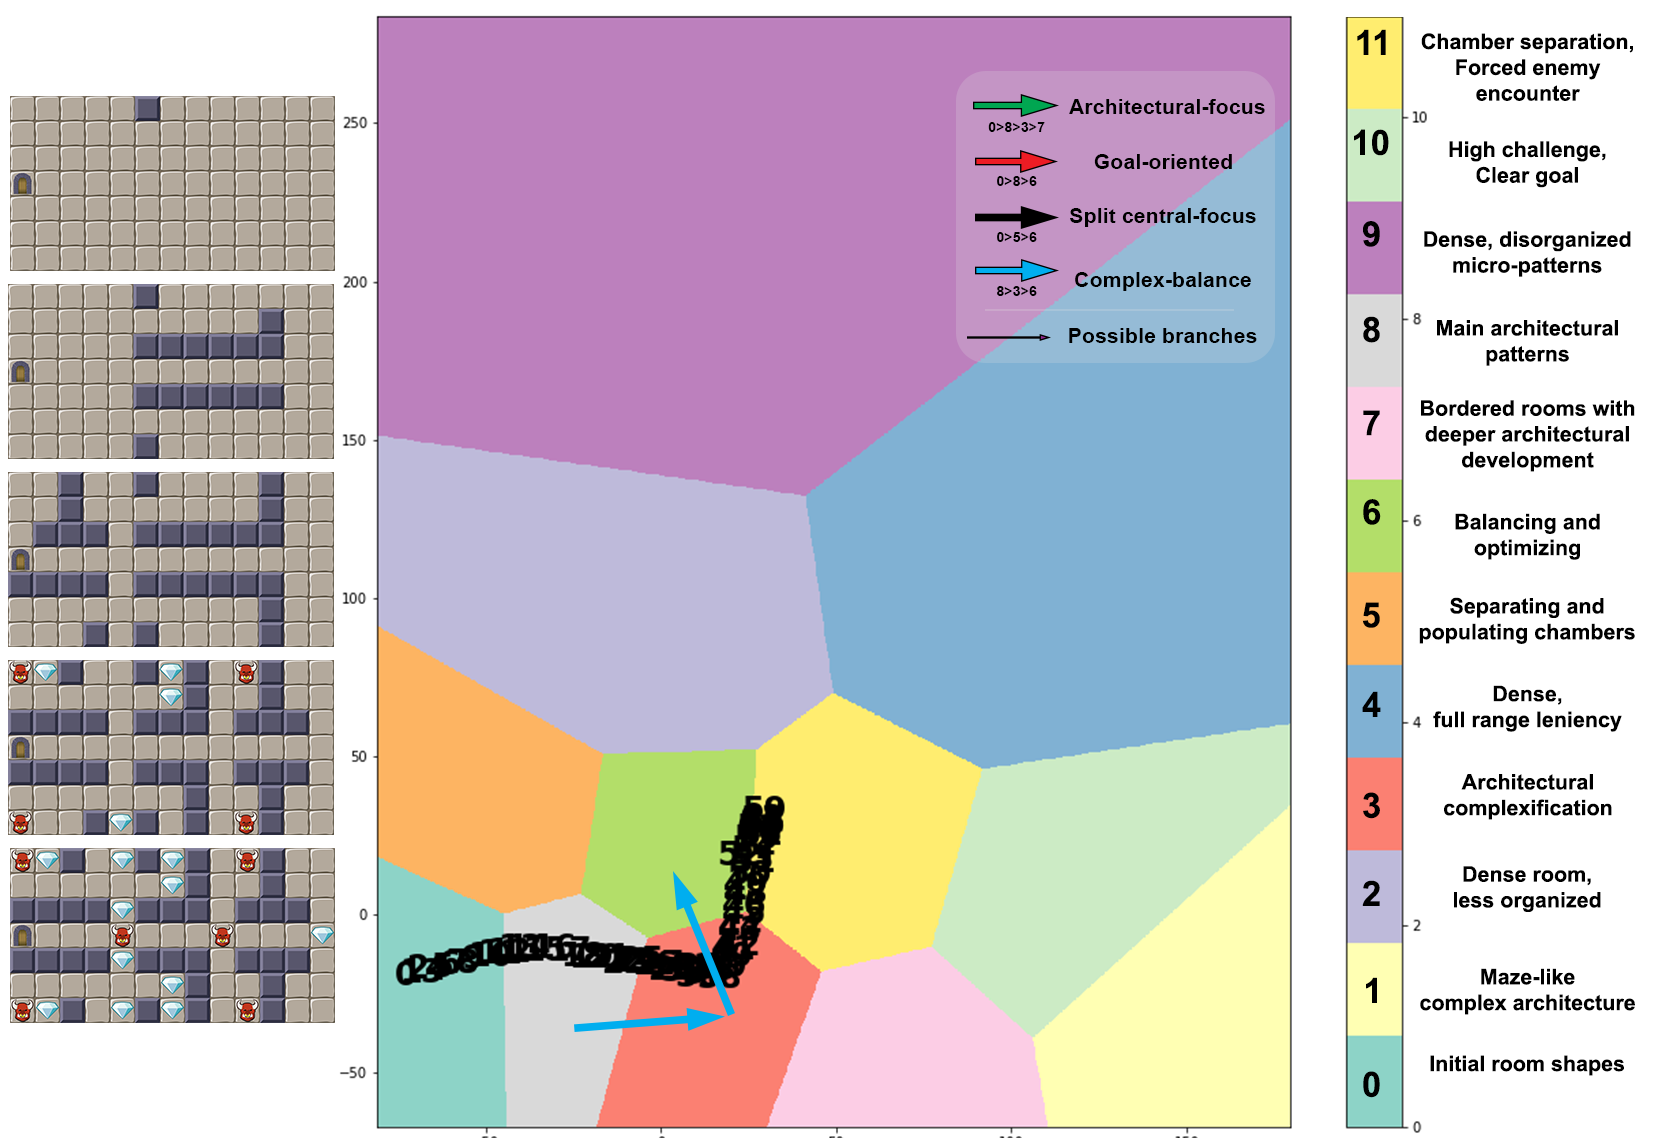
\includegraphics[width=0.45\textwidth]{figures/4.png}
     }
    
    \caption{Examples of each of the archetypical paths from one of the frequent sequences used to create the clusters. To the left of each subfigure, we present each key step in the trajectory i.e. when the design entered a new cluster. (a) presents the \textsc{Architectural-focus} archetypical path where the focus is firstly on creating the structural design of the rooms; the design process jumps back and forth suddenly to cluster 10 (one of the possible branches) due to the designer adding a boss, and removing it immediately. (b) presents the \textsc{Goal-oriented} archetypical path where the design focus on a minimal structure complexity and mix between adding structural changes and enemies/treasures. (c) shows the \textsc{Split central-focus} archetypical path where, intentionally, the designer creates a center obstacle with a boss and build around it. Finally, (d) presents the \textsc{Complex-balance} archetypical path; the design focuses on building complex, uncommon structures first and then add some goal to it with enemies and treasures, taking advantage of the spaces.}
    \label{p6fig:archetypical-examples}
\end{figure*}


Once we created, evaluated, and labeled the clusters, we were able to cluster and visualize the paths of a typical design session. Figure \ref{p6fig:paths-designers} presents an example of the design sessions, where we cluster each step of the design. This sequential process revealed that there is an interesting continuity between clusters, even capturing when a designer probably applied one of the procedural suggestions due to bigger steps in the design style clusters. Further, through this process, we could understand the progress of designers in their design process and represent their trajectory in relation to the traversed clusters rather than individual editions.

\subsubsection{Unique Trajectories}

Using the clusters in Figure \ref{p6fig:all-clusters}, we clustered the design session of all the $180$ designs and collected the unique trajectories that arose from traversing the various clusters. These unique trajectories varied in the starting point, length, and end-point, however, when analyzing the trajectories we identified common patterns among them. They had a similar shape as the following $Unique=$\{0\textgreater8\textgreater4\textgreater7\textgreater10\}, where the first and last element of the sequence are respectively, the starting- and end-points, with all the unique intermediate steps in between.

To gather the common patterns from the trajectories, we applied the Generalized Sequential Pattern (GSP) algorithm, which locates frequent subsequences in the analyzed trajectories. For instance, given three trajectories (a) \{5\textgreater1\textgreater3\textgreater11\textgreater9\}, (b) \{5\textgreater1\textgreater3\textgreater11\textgreater4\, and (c) \{0\textgreater1\textgreater3\textgreater11\}, none of these is a perfect match in its entirety, but GSP can spot that subsequences \{1\textgreater3\textgreater11\}, \{1\textgreater3\}, \{3\textgreater11\}, among others, appear with frequency $= 3$.

%(2) obtain only 1 pattern ($\{5>1>3>11\}$) with frequency=2, if searching from starting points. Finally, using GSP, we find $\{5>1>3>11\}$, $\{1>3>11\}$, $\{1>3\}$, $\{3>11\}$

%We collected these unique trajectories, and 
Furthermore, after doing a preliminary analysis, we identified some steps that we classified as ``border designs'': steps that are borderline between two clusters. These \textit{border designs} disrupted the sequence pattern mining by creating noise in the unique trajectories, specifically when these \textit{border designs} entered a different cluster for just a few steps. %we categorize them as when these "unique" noisy steps were brief.
Therefore, we filtered them out by applying a threshold $\theta = 3$, so that all subsequences inside one cluster with less than $\theta$ steps are removed from the main sequence. I.e, the sample trajectory \{0\textgreater0\textgreater0\textgreater0\textgreater8\textgreater8\textgreater8\textgreater6\textgreater8\} turns into \{0\textgreater8\} instead of \{0\textgreater8\textgreater6\textgreater8\}. Through this, we were able to reduce the noise and the search space, obtaining more meaningful and frequent patterns.

\subsubsection{Archetypical Paths through Style Space}

%Figure \ref{p6fig:finalPaths} shows the archetypical paths taken by designers when creating rooms. Represented as arrows to denote direction, 

%From all the collected unique trajectories, we identified 4 main archetypical paths, which are the ones taken most frequently by designers either as their full path or as the initial path. In Figure \ref{p6fig:finalPaths}, it is shown the archetypical paths, represented as thicker arrows to denote direction, that represent the taken by designers when creating rooms. 

In Figure \ref{p6fig:finalPaths}, we present the archetypical paths, represented as thicker arrows to denote direction, which show the most frequent paths taken by designers either through their whole design process or as the initial meaningful steps. From all the collected unique trajectories, we have identified 4 main archetypical paths, labelled, \textsc{Architectural-focus}, \textsc{Goal-oriented}, \textsc{Split central-focus}, and \textsc{Complex-balance}. In addition, we have numbered each cluster for easier visualization and referencing. 

Moreover, in the figure, it can also be observed thinner purple arrows pointing to different clusters from several of the clusters that are part of the main paths. These are \textit{possible branches} presented in the unique trajectories and added based on their frequency. Through these possible branches, the design of an archetypical session, can vary and extended or deviate the final design. Each archetypical path is defined and explained as follows: 

\paragraph{Architectural-focus}The path followed by this archetype focuses first on designing the architecture of the room with walls. Through this, the design focuses on shaping the visual patterns, chambers, and corridors to give a clear space for adding goals and objectives with enemies and treasures. The sequence is denoted with a green arrow in Figure \ref{p6fig:finalPaths}, and following the sequence \{0\textgreater8\textgreater3\textgreater7\}.

\paragraph{Goal-oriented}Design processes following this archetypical path, create the rooms in a more standard way, combining simpler symmetric wall structures with distributed placement of enemies and treasures. Thus, rather than focusing extensively on an individual part of the room, the rooms have an initial structure and then they are populated with some specific goal-in-mind. The sequence is denoted with a red arrow in Figure \ref{p6fig:finalPaths}, and following the sequence \{0\textgreater8\textgreater6\}.

%Thus, rather than focusing on an individual part of the room until satisfied, the rooms have some initial structures that are populated and continue through an iterative process between these steps.% rooms go through an iterative process of adding have some initial structures that are

\paragraph{Split central-focus}This archetypical path focuses on designing rooms with obstacles placed in the center of the room in the shape of enemies, treasures, or wall structures that clearly split the room into different areas. The design process is less organized than the other archetypes since it searches to achieve the split goal with any of the available tiles. The sequence is denoted with a black arrow in Figure \ref{p6fig:finalPaths}, and following the sequence \{0\textgreater5\textgreater6\}.
%, since the middle step is cluster 5 ("Separating and populating chambers"), which relates to rooms which are expected since the cluster 5 ("Separating and populating chambers") relate to rooms that  as specific structural shapes are not necessary. 

\paragraph{Complex-balance}This archetypical path focuses on building complex symmetric shapes with a clear objective for the player and adapting the spaces with a balance of enemies and treasures. In general, the rooms created following this path are more unique and typically balanced. %   with that adapt well. The process is quite 
The sequence is denoted with a blue arrow in Figure \ref{p6fig:finalPaths}, and following the sequence \{8\textgreater3\textgreater6\}.

Furthermore, using these archetypical paths, we can then categorize certain clusters as key clusters or being more relevant than others based on their contribution to the paths, their frequency, and their usage. Most of the paths go through or end in cluster 6 (``Balancing and optimizing'') and cluster 8 (``Main architectural patterns''), which relate to rooms that have a more explicit mix between corridors and small chambers and more clear architecture. The rooms in those clusters are or shaped as end rooms, as in the case of cluster 6, or architecturally shaped to be “optimized” to a specific goal e.g. a dense bordered room. Similarly, most of the sequences start from cluster 0 ("Initial room shapes"), with $134$ out of the $180$ designs, which correlates to the type of designs encountered in that clusters. Thus, it is understandable that most of the archetypical paths pass through any of these three clusters. 

Nevertheless, it is the steps in-between what creates a clear differentiation between the archetypical paths, which is the benefit of observing the design process as a whole in the clustered room style space. For instance, in fig.~\ref{p6fig:finalPaths}, it can be observed that \textsc{Split central-focus} starts in the same cluster as three other paths, and tentatively ends in the same cluster as three other. However, the designs following \textsc{Split central-focus} are more different to the other trajectories, since it enters a cluster that is denser with several tile types in principle, and where designers seem to have a clearer goal.
% With this, we can further understand why \textsc{Split central-focus} is more different to the other trajectories, since it enters a cluster that is "less organized" in principle. 

%Furthermore, we can also observe that certain clusters are key steps for most paths because they are or a frequent starting or ending point. Most of the paths go through or end in cluster 6 ("Balancing and optimizing") and cluster 8 ("Main structural patterns"), which relate to rooms that have a more explicit mix between corridors and small chambers and a more clear structure, thus, it is understandable since the rooms in those clusters are or shaped as end rooms, as in the case of cluster 6, or structurally shaped to be “optimized” to a specific goal (E.g. dense bordered room, maze-like, more challenging, etc.). However, the distribution of endpoints is quite even, and meanwhile, cluster 6 and cluster 11 ("Chamber separation, Forced enemy encounter") are the most frequent ending points with $36$ and $25$ out of $180$ design processes, the rest of clusters are quite close.

%Similarly, most of the sequences start from cluster 0 ("Initial room shapes"), with $134$ out of the $180$ designs, which correlates to the type of designs encountered in those clusters.

Moreover, in figure~\ref{p6fig:archetypical-examples}, we present examples of each of the designer personas by visualizing the sequence of steps done in representative design sessions, showing how these paths would look like in practice. Each visualization of a designer persona has the key design steps to the left, where each image is in a sequence: the first is the first edition of the designer, the last is the final edition, and the in-between represent entering a new room style cluster. 

In (a), it is shown the \textsc{Architectural-focus}, where the designer first created the border of the room with a clear chamber division. As the designer adds and subsequently removes the boss, the design jumps to cluster 10, which is one of the possible branches, adding a high challenge. In (b), it is shown the \textsc{Goal-Oriented}, where the designer sketched the main shape of the room followed by alternating between enemies, treasures, and walls to design the goal of the player within the room. In this example, the designer ends the design close to cluster 9, with a disorganized placement of tiles and a less aesthetical room, but forming small choke areas balancing the placement of enemies and treasures.

In (c), it is shown the \textsc{Split Central-focus}, where the designer directly started by adding a boss in the center of the room and using this as a reference point, shaped the rest of the room. In (d), it is shown the \textsc{Complex-balance}, where the designer focused on creating an uncommon structure and followed by adding enemies and treasures symmetrically, with clear individual areas for the player to approach.

% It is not surprising to focus on the center as it 

Finally, further analyzing figure~\ref{p6fig:archetypical-examples}, it can also be observed an interesting dual tendency of the designers in the archetypical paths. This dual tendency is to either focus on the aesthetic configuration of the room based on what is perceived in the editor exemplified the personas: \textsc{Architectural-focus} and \textsc{Split central-focus}, and to focus on the player experience exemplified the personas: \textsc{Goal-oriented} and \textsc{Complex-balance}. Nevertheless, both are not mutually exclusive, instead this illustrates adequately the dualistic role the designer has when using the tool and designing rooms. That of creating an aesthetically pleasing object as it is seen in the editor, and that of creating an experience.% However, this is not mutually exclusive. Instead, it shows 


% Furthermore, when analyzing how the different design sequences were clustered and forming the designer personas, we observed an interesting dual tendency of the designers. This dual tendency is to either focus on the aesthetic configuration of the room based on what is perceived in the editor through the personas: \textsc{Architectural-focus} and \textsc{Split central-focus}, and to focus on the player experience through the personas: \textsc{Goal-oriendted} and \textsc{Complex-balance}. This exemplified quite good 
% dualistic role 
% When forming the designer personas, and analyzing how different design sequences


%where the designer focused on creating the shape of the room before adding any enemyfirst created the border of the room

% Finally, in Figure \ref{p6fig:archetypical-examples}, we present examples of each of the archetypical paths to show how would these paths look like in practice, further supporting our findings and path definitions. 

% The archtypical paths a dual tendency of the designers to either go for a strategy that reflects their perception of the level from the editor - like the aesthetic configurations of it, instead of the experiential ones. for example the ones that had a split central focus and a structural focus (which btw maybe i would change to architectural focus). and then there's the ones that have a focus on the player experience like the goal oriented and complex behavior ones. i think this split reflex a very nice dualistic role that the designer has in front of the editor - that of creating an aesthetically pleasing object, as they see it in the editor, and that of creating an experience.
% , and exmplified
%That build around



% Notice that not all the clusters have connectionthat based on the unique trajectories, where designers decided to move towards other areas. 

%it is shown the archetypical paths, represented as thicker arrows to denote direction, that represent the taken by designers when creating rooms. 
% moving from 6 to 11 or from 3 to 11 is a fairly frequent step, thus making it and cluster 6, key points.
% In fact, ending the design at 7 is not that common, thus, 



% the red cluster with $95$ out of the $180$, and from the purple cluster with $49$ out of the $180$, which correlates to the type of designs encountered in those clusters, mainly emptier rooms with initial sketches and shapes. 

% Most of the paths start in cluster 0 ("Initial room shapes") 

% From the figure, we can extract the following clusters as key steps for most of the patterns: "light green", "light blue", "red", and "purple". 

% It can be observed that most of the paths end or go through the "light green" and "light blue" clusters. Both relate to rooms that have a more clear structural pattern and more explicit mix between corridors and small chambers, thus, is understandable since the rooms in those clusters are or shaped as end rooms or structurally shaped to be “optimized” to a specific goal (E.g. dense bordered room, maze-like, more challenging, etc.). Quantitatively, most of the sequences end up in those clusters, $64$ out of the $180$ end in cluster 6 (light blue) and $52$ out of the $180$ end in cluster 11 (light green).


% Similarly, most of the sequences start from the red cluster with $95$ out of the $180$, and from the purple cluster with $49$ out of the $180$, which correlates to the type of designs encountered in those clusters, mainly emptier rooms with initial sketches and shapes. 


% \begin{figure*}
% \centerline{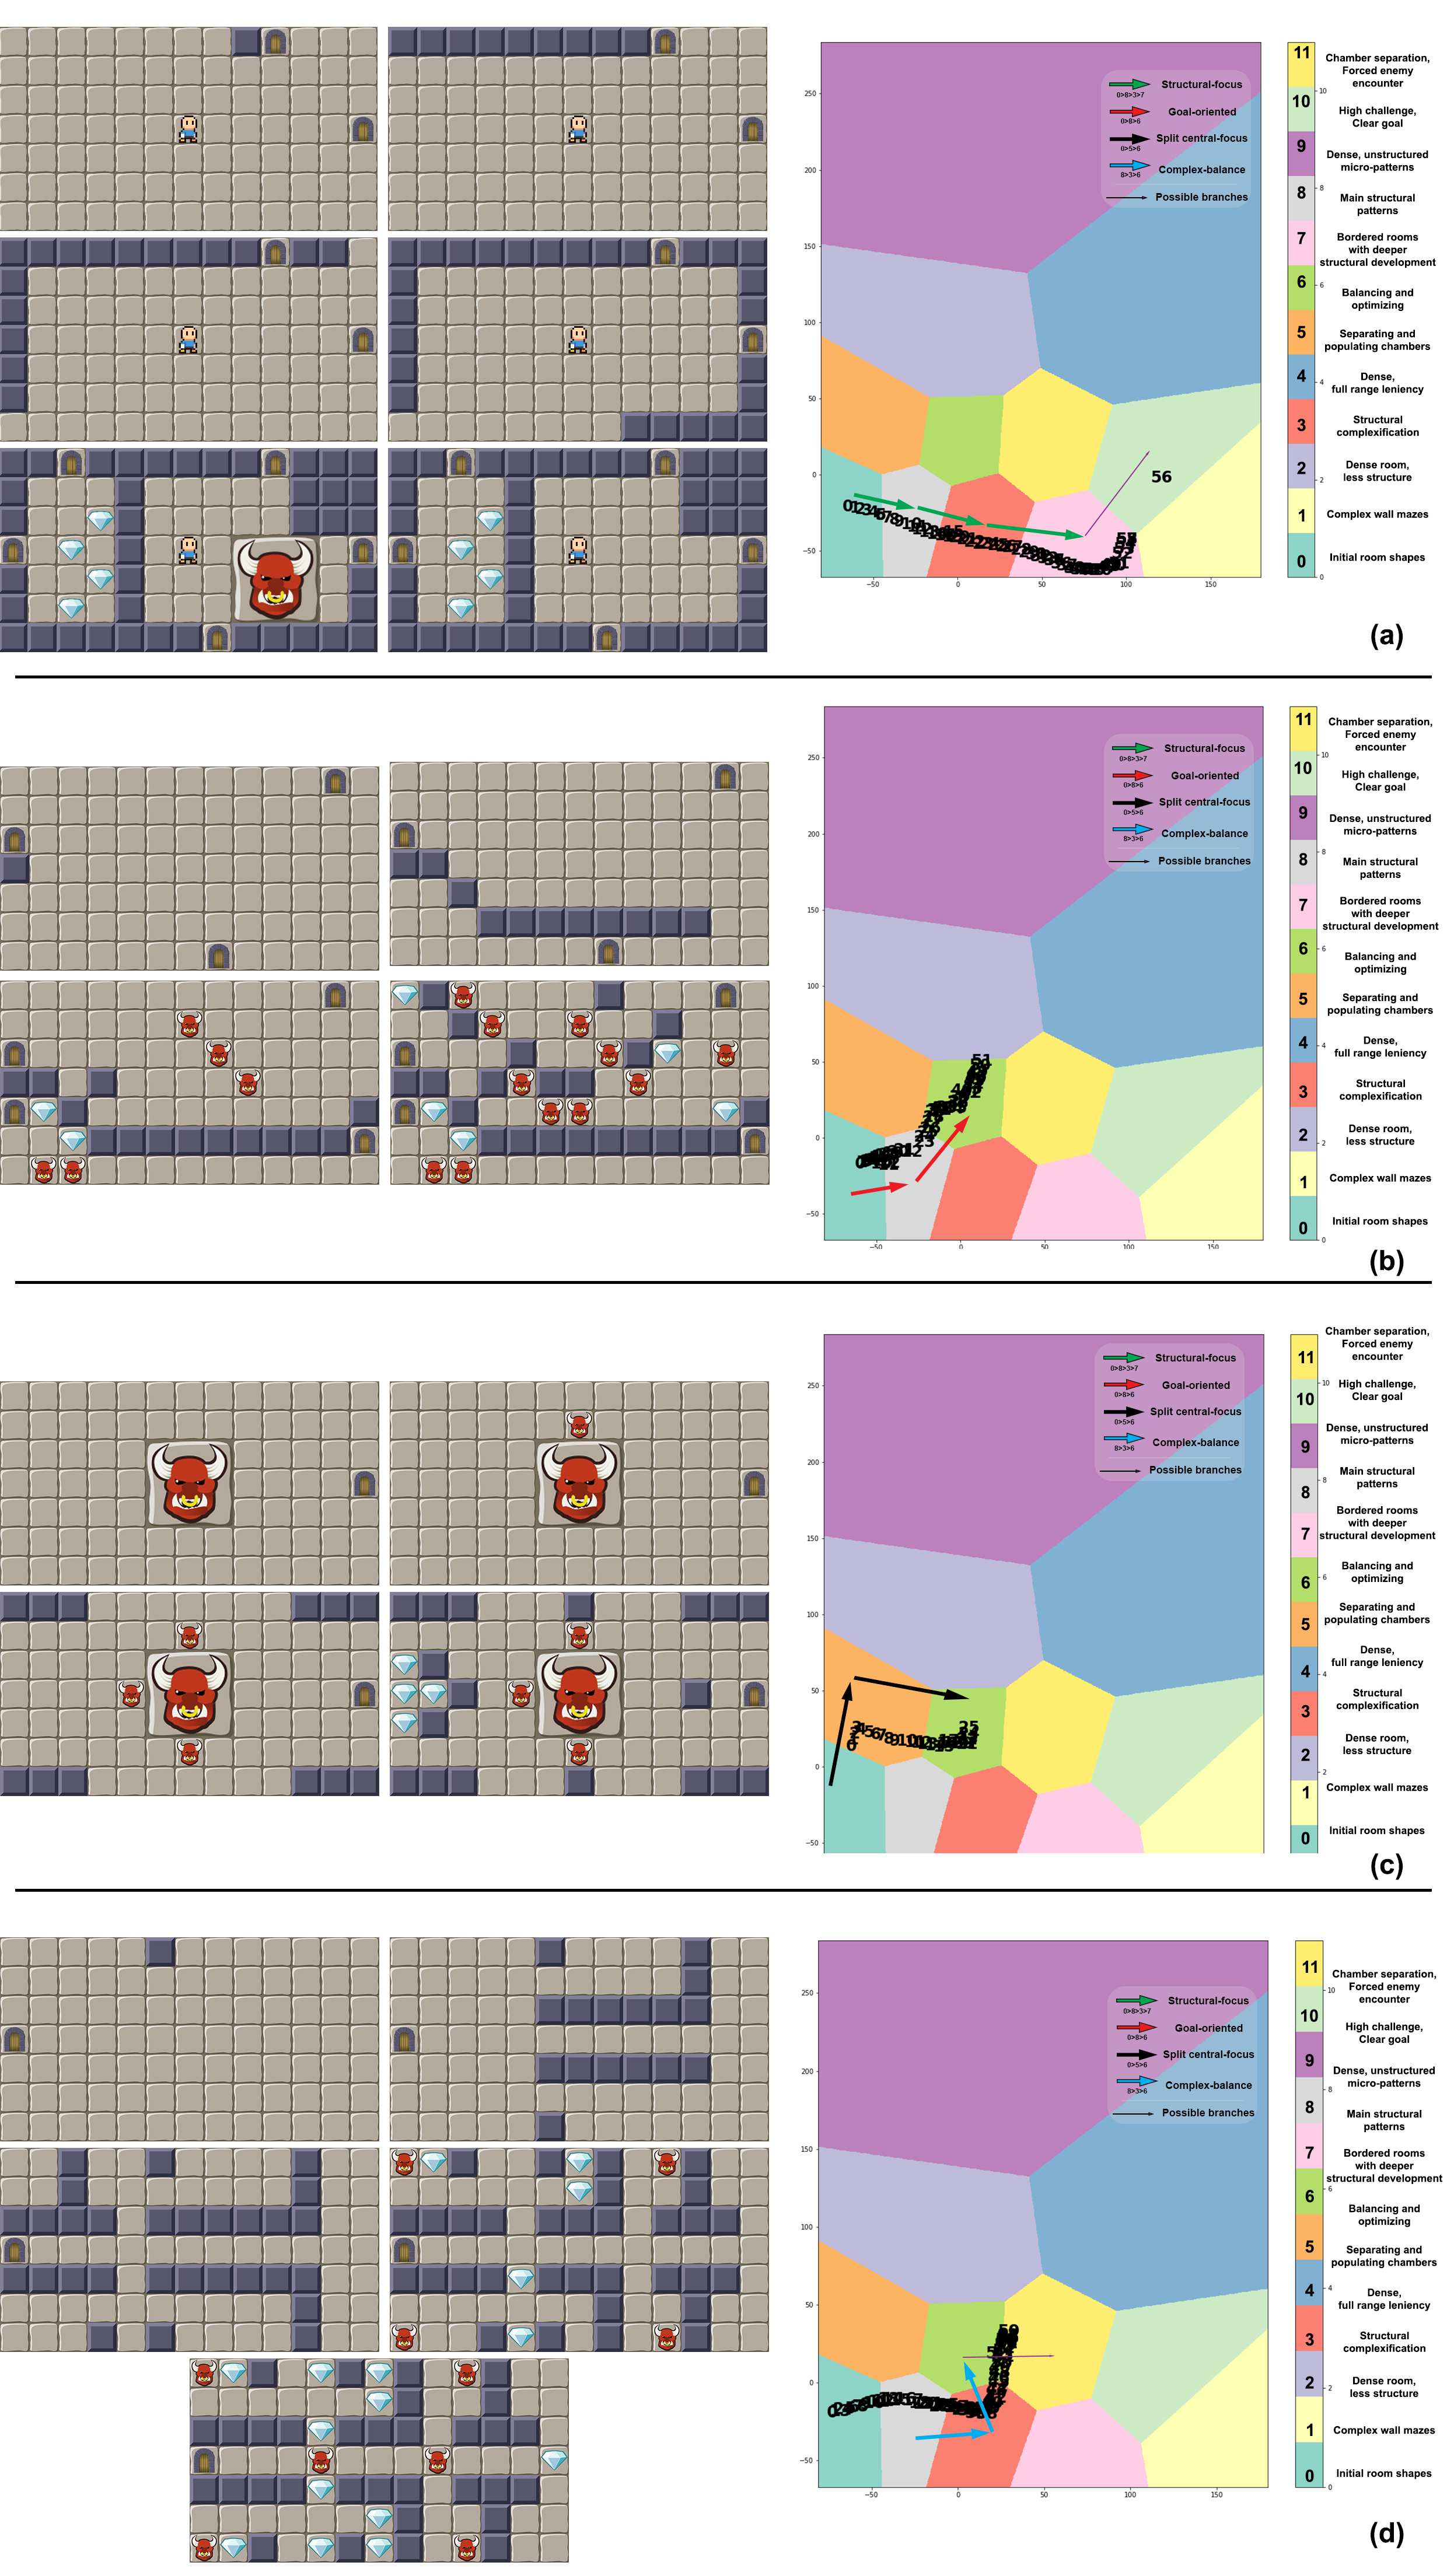
\includegraphics[width=0.7\textwidth]{figures/path-examples-2.png}}
% \caption{Examples of each of the archetypical paths from one of the frequent sequences used to create the clusters. To the left of each subfigure, we present each key step in the trajectory i.e. when the design entered a new cluster. (a) presents the \textsc{Structural focus} archetypical path where the focus is firstly on creating the structural design of the rooms; the design process jumps back and forth suddenly to cluster 10 (one of the possible branches) due to the designer adding a boss, and removing it immediately. (b) presents the \textsc{Goal-oriented} archetypical path where the design focus on a minimal structure complexity and mix between adding structural changes and enemies/treasures. (c) shows the \textsc{Split central-focus} archetypical path where intentionally, the designer creates a center obstacle with a boss and build around it. Finally, (d) presents the \textsc{Complex-balance} archetypical path; the design focuses on building complex uncommon structures first and then add some goal to it with enemies and treasures, taking advantage of the spaces.} \label{p6fig:archetypical-examples}
% \end{figure*}



% \begin{subfigure}[t]{0.33\textwidth}
%         \centering
%         \includegraphics[width=0.95\textwidth]{figures/1.png}
%         \caption{Linearity-\#MesoPatterns}
%     \end{subfigure}%
%     \begin{subfigure}[t]{0.33\textwidth}
%         \centering
%         \includegraphics[width=0.95\textwidth]{figures/1.png}
%         \caption{Linearity-\#MesoPatterns}
%     \end{subfigure}%
%     \begin{subfigure}[t]{0.33\textwidth}
%         \centering
%         \includegraphics[width=0.95\textwidth]{figures/1.png}
%         \caption{Linearity-\#MesoPatterns}
%     \end{subfigure}%
%     \begin{subfigure}[t]{0.33\textwidth}
%         \centering
%         \includegraphics[width=0.95\textwidth]{figures/1.png}
%         \caption{Linearity-\#MesoPatterns}
%     \end{subfigure}%

%From the figure, it can be observed that most of the paths end or go through the "light green" and "light blue" clusters. Both relate to rooms that have a more clear structural pattern and more explicit mix between corridors and small chambers, thus, is understandable since the rooms in those clusters are or shaped as end rooms or structurally shaped to be “optimized” to a specific goal (E.g. dense bordered room, maze-like, more challenging, etc.). Further, most of the sequences end up


%Most of the rooms end there, 64 end in cluster 6 (light blue) and 52 end in cluster 11 (light green), so it makes sense that they are key steps in most of the subsequences. Further, most of the rooms start in cluster 0 (red) – 95 rooms – or in cluster 8 (purple) – 49 rooms, which make them key steps as well

%Most of the sequences with $95$ out of the $180$ starting in the red cluster, and $49$ out of the $180$ starting in the purple cluster. which correlates to the type of designs encountered in those clusters, mainly emptier rooms with initial sketches and shapes. 


%Info about the trajectories, 1) variation (length), 2) starting cluster, 3) end-point cluster.


% \begin{itemize}
%     \item[\textbf{DONE:}] Present 3 representative examples where we cluster each step of the design process. Perhaps I should create a room that would go through all the clusters?
%     \item[\textbf{DONE:}] Explain that we did this for all the 180 designs, and we collected the unique trajectories along the clusters, reducing the dimensionality of each step to each cluster.
%     \item[\textbf{DONE:}] Due to border designs (step that are in the border between 2 different clusters), we applied a threshold to reduce the noise those inputs could have when clustering the trajectories of the designer.
%     \item[\textbf{DONE:}] this data (the sequences) were then applied the GSP algorithm, a subsequence frequent pattern mining algorithm, to extract the frequent patterns in the sequences (including subsequences within the sequence).
%     \item This resulted in the following trajectories, which can also be observed in Figure X.
%     \item 
% \end{itemize}

\subsection{Conclusions}



% \begin{itemize}
%     \item Discussion on what does this archetypical design trajectories mean?
%     \item how to use them? next steps into integrating this into a system. To use this in a search-based approach as objectives for the generation to move towards the directions where (according to our archetypical design trajectories) the designers will move towards in their design process. Perhaps I could also bring the discussion from the workshop-paper for HC-AI.
%     \item discussion on creativity? is the output or the process where the actual creativity is outputted? Compare using end-design clustering to using sequences to cluster.
%     \item Discussion on how PCGRL relates to this type of work? --> Perhaps this is something for the background instead.
% \end{itemize}{}


% This paper presents a step towards designer modelling in a MI-CC environment by providing an implementation of designer personas as archetypical trajectories through style space, as a means to characterize several representative and frequent design styles together. 

%This paper presents a novel approach and meaningful steps towards designer modeling in an MI-CC environment. By providing an implementation of designer personas as archetypical trajectories through style space, we show that 

This paper presents a novel approach and meaningful steps towards designer modeling through an experiment on archetypical design trajectories analysis in an MI-CC environment. Through this, we characterize several representative design styles as designer personas. We have first run and compared several clustering setups to find the best partitioning of the design style using the edition sequences of the collected $180$ unique rooms, ending in $8196$ data points, and resulting in a set of twelve cohesive, coherent, and meaningful clusters. We have then mapped these $180$ design sequences in terms of these clusters, applying frequent sequence mining to find four frequent and unique designer styles, with related common sub-styles. As a result, we have presented a roadmap of design styles over a map of data-driven design clusters. 

%This paper presents a step towards designer modeling through an experiment on archetypical design trajectories analysis in an MI-CC environment, as a means to characterize several representative design styles as designer personas. We have first run and compared several clustering setups to find the best partitioning using the edition sequences of the collected $180$ unique rooms, ending in $8196$ data points, and resulting in a set of twelve cohesive, coherent, and meaningful clusters. We have then mapped these $180$ design sequences in terms of these clusters, applying frequent sequence mining to find four frequent unique designer styles, with related common sub-styles. As a result, we have presented a roadmap of design styles over a map of data-driven design clusters. %The examples in Figure \ref{p6fig:archetypical-examples}, help us to clarify 

%  namely the \textsc{Designer Personas}

% Our work draws on the ideas, concepts, and goals and concepts proposed by Liapis et al. when introducing the Designer Modeling as a model to capture multiple designer's processes. A prototype of such was implemented in the sentient sketchbook~\citepsixth{p6Liapis2014-designerModelImpl}, where it is proposed the use of interactive evolution by biasing the search space in favor of hand-crafted features of the design. we propose an alternative and novel route to designer modeling through clustering the design space and the room style based on the collected data. Moreover, we differ as well on the type of level design, being the sentient sketchbook a tool for strategy games~\citepsixth{p6liapis_generating_2013}, while EDD a tool for adventure and rogue-like games~\citepsixth{p6Alvarez2020-ICMAPE}. These differences strengthen the importance and usefulness of designer modeling, and highlight the holistic and generic properties of this designer-centric perspective.

Designer modeling was proposed as an approach to capture multiple designer's processes to create a better workflow by Liapis et al.~\citepsixth{p6Liapis2013-designerModel}, and our work draws on many of their ideas, concepts, and goals. Furthermore, a prototype of such was implemented in the sentient sketchbook~\citepsixth{p6Liapis2014-designerModelImpl}, where it is proposed different approaches to model style, process, and goals based on choice-based evolution and the designer's current design to adapt the provided suggestions accordingly. We propose an alternative route to designer modeling through clustering the design space and the room style based on the collected data. Moreover, we differ in the type of level design, being the sentient sketchbook a tool for strategy games~\citepsixth{p6liapis_generating_2013}, while EDD is a tool for adventure and rogue-like games~\citepsixth{p6Alvarez2020-ICMAPE}. These differences strengthen the importance and usefulness of designer modeling and highlight the holistic and generic properties of this designer-centric perspective and its possibilities.

% Designer modeling in computer-aided design tools was proposed by Liapis et al.~\citepsixth{p6Liapis2013-designerModel} as an approach to capture multiple designer's processes to create a better workflow, and a prototype of such was implemented in the sentient sketchbook~\citepsixth{p6Liapis2014-designerModelImpl}. While our work drags on many of the concepts, ideas, and goals described by Liapis et al., we propose an alternative route to designer modeling through clustering the design space

% In their work, they propose the use of hand-crafted

% Our work drags on many of the concepts, ideas, and goals described in~\citepsixth{p6Liapis2013-designerModel}, but we propose an alternative route to designer modeling through clustering the design space and the room style based on the collected data. In contrast 

% Their work propose the use of interactive evolution by biasing the search space in favor of hand-crafted features of the design akin to~\citepsixth{p6Alvarez2020-DesignerPreference}. However, we propose an alternative and novel route to designer modeling through clustering the design space and the room style based on the collected data. Moreover, we differ as well on the type of level design, being the sentient sketchbook a tool for strategy games~\citepsixth{p6liapis_generating_2013}, while EDD a tool for adventure and rogue-like games~\citepsixth{p6Alvarez2020-ICMAPE}. Applying the idea of designer modelling to both genres, not only shows the importance and usefulness of designer modeling but also the holistic and generic view 

% These differences strengthen the importance and usefulness of designer modeling, and highlight the holistic and generic properties of this designer-centric perspective.

% % might be interesting to discuss this.
% While the approach described in this paper is applied in a tool for creating zelda-like dungeon games~\citepsixth{p6tloz}, the approach can be reused and extended to other domains 

These contributions allow us to better understand, cluster, categorize and isolate designer behavior. This is very valuable for mixed-initiative approaches, where a clear virtual model of the designer's style allows us to better drive the search process for procedurally generating content that is valuable for the designer. Designer personas have the potential to be used in many different scenarios. For instance, as objectives for a search-based approach to enable a more style-sensitive system, to evaluate the fitness of evolutionary generated content or to train PCG agents via Reinforcement Learning~\citepsixth{p6khalifa2020-pcgrl}. 

Moreover, recognizing the designers' current style and the path taken so far, which would indicate a possible designer persona, could open the possibility for recognizing their intentions, preferences, and goals. This traced roadmap of designer personas could let a content generator anticipate a designer's next moves without heavy computational cost, just by identifying her current location on the map and offering content suggestions that lie in the most promising clusters to be visited next. Conversely, it could also identify designers who do not follow a certain path, i.e. deviating from the pattern, trying to understand their objective through their design style.

% Finally, in our work, we did not observe any type of cross-path i.e. a design going from one path to another. We believe that this is due to the level at which we observe the archetypical paths. However, preliminary analysis on the dataset used in this paper and as expected, the design process of designed rooms within the same dungeon does follow different paths, and sometimes even crossing each other. This opens an interesting and exciting area to explore a wider layer, taking rooms as a set of archetypical paths taken by designers. Observing the paths taken in previous and future rooms, and the dungeon as a whole, as briefly introduced in section~\ref{p6sec:designStyle}, to understand the designers' intentions and goals when they proceed to create a new room is a promising future step to take with the current system. 

%  i.e. room-wise, as the designer typically would design the room with a set of goals

Finally, it is also important to observe the nature of the previous and future rooms created by a designer. Observing the dungeon as a whole, as briefly introduced in section~\ref{p6sec:designStyle}, to understand the designers' intentions and goals when they proceed to create a new room is a promising future step to take with the current system. 

% Furthermore, the designer personas addresses the dynamic-dynamic system vs. dynamic-static system open question raised by Alvarez and Font~\citepsixth{p6Alvarez2020-DesignerPreference}, which relates to the challenge of adapting a system to the a ever-changing designer. With the use of the archetypical paths, the model is not anymore adapting and moving through the solution space with the designer, rather the designer traverse through an already clustered space. 

% With the use of the archetypical paths, we can not only identify the current designer persona the designer is following but we can also adapt and anticipate to what they might end up doing. 

% Furthermore, the designer personas addresses an open question raised by Alvarez and Font \citepsixth{p6Alvarez2020-DesignerPreference}, related to the challenges  using a dynamic-dynamic system vs. a dynamic-static system. The authors describe the dynamic-dynamic system as a system where both designer and AI-system move through the solution space, with the AI-system constantly trying to adapt to the designer. They concluded that the main challenge correspond to designers constantly concept drifting resulting in them continuously changing their decisions. Instead, the authors proposed the use of a dynamic-static system, where the model is not anymore adapting and moving through the solution space with the designer, rather the designer traverse through an already clustered space. With the use of the archetypical paths, we can not only identify the current designer persona the designer is following but we can also adapt and anticipate to what they might end up doing. 


%and conclude that the main challenges in

% Moreover, this traced roadmap of designer personas could let a content generator anticipate a designer's next moves without heavy computational cost, just by identifying her current location on the map and offering content suggestions that lie in the most promising clusters to be visited next. %Further, one could also be able to identify designers that do not follow a certain path i.e. deviating from the pattern, and try to understand through their design style their objective.





% From the $180$ unique rooms, we extracted and used the edition sequence of each of the rooms, from their initial design to the more elaborated end-design, to compose a richer dataset that could capture the design process of a designer rather than focusing on the end-point. Through this, we ended up using $8196$ data points in our dataset.

% We have first run and compared s


% through experimenting with 

% This paper presents a step towards designer modelling by providing a prototype implementation of designer personas as archetypical trajectories through style space. These archetypical paths

% This paper presents an experiment on archetypical design trajectories analysis in a MI-CC environment, as a means to characterize several representative design styles as designer personas. We have first run and compared several clustering setups to find the best partitioning, resulting into a set of twelve cohesive, coherent, and meaningful clusters. We have then mapped almost 200 complete design sequences in terms of these clusters, applying sequence mining to find four frequent unique designer styles, with related common sub-styles. As a result, we have presented a roadmap of design styles over a map of data-driven design clusters. 



% be used as goal for other systems were anticipating a design or creating a synthetic objective might be more complicated. We envision that these designer personas can be used within 

\bibliographystylepsixth{ieeetr}
\bibliographypsixth{included-papers-tex/paper-6/references.bib}




% \clearpage
% \phantomsection
% \addcontentsline{toc}{section}{PAPER 1}
% \includepdf[pages=-]{included-papers/paper1.pdf}

% \clearpage
% \phantomsection
% \addcontentsline{toc}{section}{PAPER 2}
% \includepdf[pages=-]{included-papers/paper2.pdf}


% \clearpage
% \phantomsection
% \addcontentsline{toc}{section}{PAPER 3}
% \includepdf[pages=-]{included-papers/paper3.pdf}


% \clearpage
% \phantomsection
% \addcontentsline{toc}{section}{PAPER 4}
% \includepdf[pages=-]{included-papers/paper4.pdf}


% \clearpage
% \phantomsection
% \addcontentsline{toc}{section}{PAPER 5}
% \includepdf[pages=-]{included-papers/paper5.pdf}


% \clearpage
% \phantomsection
% \addcontentsline{toc}{section}{PAPER 6}
% \includepdf[pages=-]{included-papers/paper6.pdf}

